% ==============================================================================
% FILE PRINCIPALE — Ricerca Bibliografica sulle Spiking Neural Networks (SNN)
% Compilazione consigliata:
%   pdflatex main && biber main && pdflatex main && pdflatex main
% oppure: ./compila.sh
% ==============================================================================
\documentclass[11pt, a4paper]{article}

% ==============================================================================
% PREAMBOLO — Stile accademico LaTeX classico (sobrio, bianco e nero standard)
% ==============================================================================
\usepackage[T1]{fontenc}
\usepackage[utf8]{inputenc}
\usepackage[italian]{babel}
\usepackage{csquotes}
\usepackage{lmodern}
\usepackage{microtype}

% Geometria pagina standard bilanciata
\usepackage[
  a4paper,
  top=2.5cm,
  bottom=2.5cm,
  left=2.4cm,
  right=2.4cm
]{geometry}
\usepackage{placeins}

% Matematica e unita' di misura (standard italiano con virgola decimale)
\usepackage{amsmath, amssymb, mathtools}
\usepackage{siunitx}
\sisetup{
  locale = DE,
  output-decimal-marker = {,},
  group-separator = {\,},
  group-minimum-digits = 4,
  per-mode = symbol,
  range-phrase = {--},
  range-units = single,
  detect-all = true
}
\DeclareSIUnit\bit{bit}
\DeclareSIUnit\byte{B}
\DeclareSIUnit\spike{spike}
\DeclareSIUnit\event{evento}
\DeclareSIUnit\events{eventi}
\DeclareSIUnit\ch{ch}
\DeclareSIUnit\hop{hop}
\DeclareSIUnit\class{class.}

% Palette neutrale in scala di grigi (stile classico LaTeX da stampa)
\usepackage[dvipsnames, svgnames, table]{xcolor}
\definecolor{NavyPrimary}{gray}{0.10}
\definecolor{TealAccent}{gray}{0.25}
\definecolor{CoralAccent}{gray}{0.20}
\definecolor{AmberAccent}{gray}{0.35}
\definecolor{SlateText}{gray}{0.15}
\definecolor{LightBg}{gray}{0.96}
\definecolor{WarmBg}{gray}{0.93}
\definecolor{TealBg}{gray}{0.94}
\definecolor{RuleGray}{gray}{0.75}

% Sfondi neutri molto tenui per i blocchi circuitali
\definecolor{BlockNMDA}{gray}{0.94}
\definecolor{BlockLEAK}{gray}{0.91}
\definecolor{BlockAHP}{gray}{0.95}
\definecolor{BlockNa}{gray}{0.92}
\definecolor{BlockK}{gray}{0.96}
\definecolor{BlockRed}{gray}{0.93}

% Grafica, figure, sottotitoli e tabelle standard
\usepackage{graphicx}
\graphicspath{{figures/}}
\usepackage{subcaption}
\usepackage{float}
\usepackage{booktabs}
\usepackage{tabularx}
\newcolumntype{L}[1]{>{\raggedright\arraybackslash}p{#1}}
\newcolumntype{Y}{>{\raggedright\arraybackslash}X}
\usepackage{multirow}
\usepackage{makecell}
\usepackage{pdflscape}
\usepackage{rotating}
\usepackage{enumitem}
\setlist{nosep, leftmargin=*, topsep=4pt}

% Didascalie standard LaTeX in nero
\usepackage[
  font=small,
  labelfont=bf,
  margin=6pt
]{caption}

% Circuiti CMOS (CircuiTikZ), diagrammi a blocchi (TikZ) e grafici (PGFPlots)
\usepackage[siunitx, RPvoltages]{circuitikz}
\ctikzset{
  transistors/scale=0.82,
  resistors/scale=0.78,
  capacitors/scale=0.78,
  sources/scale=0.78,
  amplifiers/scale=0.78,
  logic ports/scale=0.75,
  tripoles/mos style/arrows
}
\usetikzlibrary{
  arrows.meta,
  positioning,
  calc,
  fit,
  backgrounds,
  shapes.geometric,
  shapes.multipart,
  decorations.pathreplacing
}
\usepackage{pgfplots}
\pgfplotsset{compat=1.18}
\usepgfplotslibrary{groupplots}

% Riquadri di sintesi sobri in stile classico bianco/grigio
\usepackage[most]{tcolorbox}
\newtcolorbox{sintesiBox}[1]{
  enhanced,
  breakable,
  colback=gray!4,
  colframe=black!70,
  colbacktitle=gray!12,
  coltitle=black,
  fonttitle=\bfseries\small,
  title={#1},
  boxrule=0.5pt,
  titlerule=0.4pt,
  arc=1.5pt,
  left=8pt, right=8pt, top=6pt, bottom=6pt,
  before skip=10pt, after skip=10pt
}

\newtcolorbox{criticaBox}[2][]{
  enhanced,
  breakable,
  colback=gray!4,
  colframe=black!80,
  colbacktitle=gray!15,
  coltitle=black,
  fonttitle=\bfseries\small,
  title={#2},
  boxrule=0.6pt,
  titlerule=0.4pt,
  arc=1.5pt,
  left=8pt, right=8pt, top=6pt, bottom=6pt,
  before skip=10pt, after skip=10pt,
  #1
}

\newtcolorbox{notaTecnica}[1]{
  enhanced,
  breakable,
  colback=white,
  colframe=black!60,
  colbacktitle=gray!10,
  coltitle=black,
  fonttitle=\bfseries\small,
  title={#1},
  boxrule=0.5pt,
  titlerule=0.4pt,
  arc=1.5pt,
  left=8pt, right=8pt, top=6pt, bottom=6pt,
  before skip=8pt, after skip=8pt
}

% Stile di pagina standard LaTeX (numero di pagina pulito in basso, zero decorazioni)
\pagestyle{plain}

% Bibliografia con BibLaTeX + Biber (stile numerico standard)
\usepackage[
  backend=biber,
  style=numeric-comp,
  sorting=none,
  maxbibnames=6,
  minbibnames=3,
  giveninits=true,
  doi=true,
  url=false,
  isbn=false
]{biblatex}
\addbibresource{bibliografia.bib}

% Collegamenti ipertestuali cliccabili ma completamente neri (stile standard)
\usepackage[
  hidelinks,
  bookmarksopen=true,
  bookmarksnumbered=true
]{hyperref}

% Scorciatoie tipografiche utili e coerenti
\newcommand{\Vmem}{V_{\mathrm{mem}}}
\newcommand{\Vthr}{V_{\mathrm{thr}}}
\newcommand{\Vrst}{V_{\mathrm{rst}}}
\newcommand{\Vrest}{V_{\mathrm{rest}}}
\newcommand{\Vdd}{V_{\mathrm{DD}}}
\newcommand{\Cmem}{C_{\mathrm{mem}}}
\newcommand{\Csyn}{C_{\mathrm{syn}}}
\newcommand{\Isyn}{I_{\mathrm{syn}}}
\newcommand{\Imem}{I_{\mathrm{mem}}}
\newcommand{\Iin}{I_{\mathrm{in}}}
\newcommand{\UT}{U_{\mathrm{T}}}
\newcommand{\ND}{\text{N.D.}}

% Spaziatura paragrafi pulita e leggibile
\setlength{\parindent}{0pt}
\setlength{\parskip}{5pt}
\renewcommand{\arraystretch}{1.18}


% ------------------------------------------------------------------------------
% METADATI MODIFICABILI (personalizza qui i tuoi dati universitari)
% ------------------------------------------------------------------------------
\newcommand{\NomeUniversita}{Università degli Studi di Brescia}
\newcommand{\NomeDipartimento}{Dipartimento di Ingegneria dell'Informazione}
\newcommand{\NomeCorso}{Corso di Bioelettronica}
\newcommand{\AnnoAccademico}{Anno Accademico 2025/2026}
\newcommand{\NomeAutore}{Nome Cognome}
\newcommand{\MatricolaAutore}{Matricola: XXXXXX}
\newcommand{\NomeDocente}{Prof.\ Nome Cognome}

\hypersetup{
  pdftitle={Spiking Neural Networks per sistemi biomedicali impiantabili: applicazioni e architetture circuitali CMOS},
  pdfauthor={\NomeAutore},
  pdfsubject={Ricerca bibliografica di Bioelettronica su SNN, neuroni in silicio CMOS e sistemi biomedicali impiantabili},
  pdfkeywords={Spiking Neural Networks, LIF, CMOS sottosoglia, DPI, ROLLS, NET-TEN, DYNAPs, DYNAP-SE2, NeuroSEED, Xylo, bioelettronica}
}

\begin{document}

% ==============================================================================
% FRONTESPIZIO (stile universitario LaTeX classico)
% ==============================================================================
\begin{titlepage}
  \thispagestyle{empty}
  \centering
  \vspace*{0.6cm}

  {\Large\bfseries\MakeUppercase{\NomeUniversita}\par}
  \vspace{0.25cm}
  {\normalsize\NomeDipartimento\par}
  \vspace{0.15cm}
  {\normalsize\textsc{\NomeCorso}\par}

  \vspace{0.6cm}
  \rule{\textwidth}{0.6pt}
  \vspace{1.8cm}

  {\small\textsc{Ricerca Bibliografica}\par}
  \vspace{0.45cm}

  {\Huge\bfseries
    Spiking Neural Networks per sistemi biomedicali impiantabili:\\[0.35em]
    \LARGE applicazioni e architetture circuitali CMOS\par}

  \vspace{1.5cm}
  \begin{minipage}{0.88\textwidth}
    \small
    \begin{center}
      \textbf{Sintesi}
    \end{center}
    \vspace{-0.2cm}
    La presente relazione esamina le potenzialità delle \emph{Spiking Neural Networks} (SNN) per l'elaborazione locale a bassissimo consumo di biosegnali in dispositivi biomedicali impiantabili. Dopo un inquadramento sui principi del calcolo neuromorfico e sui modelli di neurone spiking — con particolare attenzione al modello \emph{Leaky Integrate-and-Fire} (LIF) e alle sue estensioni adattative — il lavoro approfondisce da un lato le applicazioni cliniche e precliniche a bassa latenza (rilevamento di crisi epilettiche e monitoraggio dell'attività neurale), dall'altro le architetture circuitali CMOS analogiche, \emph{mixed-signal} e digitali per la realizzazione fisica di neuroni e processori neuromorfici. L'analisi si conclude con una valutazione quantitativa critica sul reale vantaggio energetico a livello di sistema rispetto ai costi di acquisizione, sinapsi, memoria e interconnessioni.
  \end{minipage}

  \vfill

  \begin{minipage}[t]{0.46\textwidth}
    \raggedright
    {\small Candidato:}\\[0.25em]
    {\large\bfseries\NomeAutore}\\[0.15em]
    {\small\MatricolaAutore}
  \end{minipage}
  \hfill
  \begin{minipage}[t]{0.46\textwidth}
    \raggedleft
    {\small Docente del corso:}\\[0.25em]
    {\large\bfseries\NomeDocente}
  \end{minipage}

  \vspace{1.2cm}
  \rule{\textwidth}{0.4pt}
  \vspace{0.35cm}
  {\normalsize\AnnoAccademico\par}
\end{titlepage}

% ==============================================================================
% INDICE GENERALE, ELENCO FIGURE E TABELLE
% ==============================================================================
\pagenumbering{roman}
\tableofcontents
\vspace{0.8cm}
\listoffigures
\vspace{0.6cm}
\listoftables
\clearpage

% ==============================================================================
% CORPO DELLA RELAZIONE (file modulari in sezioni/)
% ==============================================================================
\pagenumbering{arabic}

% ==============================================================================
% SEZIONE 1 — INTRODUZIONE ALLE SNN E AI MODELLI DI NEURONE ARTIFICIALE
% ==============================================================================
\section[Introduzione alle SNN e modello LIF]{Introduzione alle SNN e modello LIF}
\label{sec:introduzione}

\subsection{Cos'è una Spiking Neural Network}
\label{subsec:paradigma}


Storicamente, i segnali biologici provenienti dagli elettrodi nei dispositivi elettronici vengono elaborati secondo l'architettura di von Neumann: il segnale viene campionato e convertito in digitale da un ADC, per poi passare ad un microcontrollore o ad un processore DSP. Questo approccio risulta inefficiente quando si devono elaborare segnali biologici lenti, sparsi nel tempo e caratterizzati da lunghi periodi di attività poco informativa (come l'elettroencefalogramma, i potenziali di campo locale o i potenziali d'azione extracellulari). Il continuo trasferimento di dati tra memoria e unità di calcolo comporta dei consumi energetici difficilmente sostenibili nei dispositivi impiantabili~\cite{qiao2015, moradi2018, bartels2025}.

Verso la fine degli anni ottanta, Carver Mead ha introdotto il concetto di ingegneria neuromorfica, che si basa sul progettare dei sistemi elettronici che emulano i principi computazionali del nostro sistema nervoso~\cite{indiveri2011}, sfruttando direttamente la fisica dei dispositivi. Un esempio sono le \emph{Spiking Neural Networks} (SNN), definite come le reti neurali di terza generazione~\cite{li2024}. Rispetto alle reti neurali tradizionali, in cui i neuroni si scambiano dei valori continui ad ogni ciclo di clock, nelle SNN l'informazione viene trasmessa con degli impulsi elettrici discreti chiamati \emph{spike} (come i potenziali d'azione biologici)~\cite{indiveri2011, li2024}. Ecco alcune caratteristiche delle SNN:
\begin{enumerate}
  \item L'informazione non è contenuta nell'ampiezza di un impulso, ma nell'istante di occorrenza e negli intervalli tra impulsi successivi (\emph{inter-spike interval}, ISI). Infatti, quando il segnale non mostra variazioni significative, la rete rimane quasi inattiva e i consumi si riducono drasticamente~\cite{indiveri2011, ronchini2023, bartels2025}.
  \item Il segnale viene elaborato in tempo reale mentre arriva, senza dover prima registrare in un buffer blocchi di campioni. Questo è possibile perché i circuiti hanno delle costanti di tempo dell'ordine dei millisecondi o decine di millisecondi, cioè gli stessi tempi dei segnali biologici~\cite{qiao2015, bartels2025}.
  \item Ogni neurone è collegato agli altri tramite le sinapsi, ovvero dei collegamenti su cui viaggiano gli spike. Ogni sinapsi ha un proprio peso, che viene memorizzato localmente, evitando così di dover leggere continuamente i pesi da una memoria esterna~\cite{qiao2015, moradi2018}.
  \item In un chip con migliaia di neuroni, è fisicamente impossibile collegare ogni neurone a tutti gli altri con dei fili dedicati. Per risolvere questo problema si usa il protocollo \emph{Address-Event Representation} (AER): ad ogni neurone viene assegnato un codice numerico univoco (quindi una specie di indirizzo); nel momento esatto in cui un neurone genera uno spike, invia il proprio indirizzo su un bus digitale condiviso, che lavora molto più velocemente dei tempi biologici (in nanosecondi) e permette di smistare gli spike ai neuroni destinatari usando pochissimi collegamenti fisici~\cite{indiveri2011, moradi2018}.
\end{enumerate}

\newpage

\subsection{Articoli di riferimento e criteri di scelta}
\label{subsec:perimetro}

Come richiesto dalla consegna, sono partito da 3 articoli di base: il primo è di Indiveri et al.\ (2011)~\cite{indiveri2011}, che illustra i principali circuiti in tecnologia CMOS usati per realizzare neuroni artificiali; presenta delle soluzioni complesse e molto vicine alla biologia, ma anche circuiti molto semplifici per ridurre area e consumi. Il secondo è lo studio di Qiao et al.\ (2015)~\cite{qiao2015}, che presenta ROLLS, un processore neuromorfico riconfigurabile che combina circuiti analogici e digitali, dotato di 256 neuroni e 128k sinapsi. Il terzo è il lavoro di Ronchini et al.\ (2023)~\cite{ronchini2023}, dedicato a NET-TEN, una rete neuromorfica analogica a bassissimo consumo progettata per rilevare gli eventi epilettici a partire dai potenziali di campo locale (LFP) registrati in vitro su tessuto cerebrale di topo.

Tra gli altri quattro articoli proposti nella consegna, ne ho scelti due per approfondire il tema della scalabilità e valutare i consumi reali. Il primo è di Moradi et al.\ (2018)~\cite{moradi2018}, che presenta il processore DYNAPs e affronta il problema di come gestire la memoria e lo smistamento degli spike quando la rete diventa grande; questo articolo è molto utile perché riporta nel dettaglio quanta area e quanta energia richiede ogni singola operazione sul chip. Il secondo è di Wu et al.\ (2026)~\cite{wu2026}, che propone NeuroSEED, un chip impiantabile che si occupa di: acquisire un segnale biologico da 32 canali; convertire il segnale in ingresso in spike; riconoscere dei potenziali d'azione e trasmettere via wireless dei dati verso l'esterno. Avere tutti questi blocchi sullo stesso chip permette di capire quanto consuma davvero un chip neuromorfico.

Ho deciso comunque di includere alla fine anche gli altri due paper della lista, perchè chiudono il cerchio sulle crisi epilettiche: l'articolo di Bartels et al.\ (2025)~\cite{bartels2025} usa il processore DYNAP-SE2 (evoluzione della famiglia DYNAP, che integra sullo stesso chip anche il circuito di acquisizione e di conversione del segnale in spike) per rilevare crisi epilettiche a partire da registrazioni EEG intracraniche umane; quello di Li et al.\ (2024)~\cite{li2024} rileva le crisi grazie a Xylo, un processore SNN interamente digitale con consumi inferiori al milliwatt, testato su registrazioni EEG di scalpo.

\subsection{Modelli matematici di un neurone artificiale}
\label{subsec:modelli_neurone}

Un neurone biologico è formato da tre parti principali:
\begin{itemize}
  \item I dendriti sono i rami d'ingresso, che ricevono i segnali provenienti dagli altri neuroni.
  \item Il soma è il corpo cellulare, che elabora i segnali in ingresso.
  \item L'assone è il canale d'uscita, lungo cui viaggiano gli spike emessi dal soma verso i neuroni successivi.
\end{itemize}

Gli spike che percorrono gli assoni dei neuroni raggiungono i punti di giunzione con i dendriti del neurone successivo, ovvero le sinapsi. Ciascuna sinapsi converte lo spike in arrivo in una piccola corrente elettrica, che può essere eccitatoria (EPSC) se tende ad attivare il neurone, oppure inibitoria (IPSC) se tende a frenarlo. Tutte le correnti ricevute si sommano nel soma caricando la membrana cellulare; se la tensione supera una certa soglia, il neurone genera a sua volta uno spike che viaggia verso i neuroni successivi~\cite{indiveri2011}. In letteratura esistono diversi modelli matematici che descrivono questo processo:

\begin{itemize}
  \item Modello di Hodgkin--Huxley (H--H): descrive in modo fedele come si comportano i canali presenti sulla membrana del neurone, cioè quei passaggi che si aprono e si chiudono in base alla tensione lasciando entrare e uscire ioni di sodio ($\mathrm{Na}^+$) e potassio ($\mathrm{K}^+$) per generare lo spike (insieme a una piccola corrente di perdita), usando un sistema di quattro equazioni differenziali non lineari~\cite{indiveri2011}. Il problema è che per realizzarlo su un chip richiede molti transistori, tanti parametri da regolare e molta area. Per questo è poco pratico per dispositivi impiantabili~\cite{indiveri2011}.
  \item Modello Leaky Integrate-and-Fire (LIF): è il modello più semplice ed efficiente dal punto di vista hardware. Descrive il neurone con tre semplici meccanismi: accumula nel tempo le correnti in ingresso facendo salire la tensione di membrana (\emph{integrate}), perde lentamente carica tornando verso il riposo se non arrivano nuovi stimoli (\emph{leaky}), e appena la tensione raggiunge una soglia prefissata emette uno spike e riporta subito la tensione al valore iniziale, di reset (\emph{fire})~\cite{indiveri2011, li2024}. Rispetto all'H-H, richiede pochissimi componenti circuitali e consuma molta meno energia.
  \item Modelli Integrate-and-Fire generalizzati: il modello LIF, essendo molto semplice, non riesce da solo a riprodurre alcuni comportamenti tipici dei neuroni reali, come l'adattamento della frequenza (Spike-Frequency Adaptation, SFA, cioè il fatto che sotto uno stimolo costante il neurone all'inizio spara veloce e poi rallenta) oppure il bursting (l'emissione di brevi raffiche di spike seguite da pause). Per ottenere questi comportamenti senza tornare alla complessità dell'H-H, si parte dal LIF e si aggiunge una seconda variabile che frena gradualmente il neurone mano a mano che spara. I tre modelli principali di questa famiglia presenti nei paper sono:
  \begin{enumerate}[label=(\alph*)]
    \item Modello di Izhikevich (2003): usa un'equazione con un termine quadratico ($\Vmem^2$) per descrivere la salita rapida dello spike assieme a una variabile lenta di recupero $U$ che riporta il neurone a riposo. Con pochi parametri riesce a imitare molti comportamenti reali ed è usato in NET-TEN~\cite{ronchini2023} e nei neuroni quadratici descritti in~\cite{indiveri2011};
    \item Modello Adaptive Exponential I\&F (AdEx-I\&F) di Brette e Gerstner (2005): modifica l'equazione del LIF aggiungendo un termine esponenziale che fa crescere molto rapidamente la tensione di membrana quando si avvicina alla soglia, e aggiunge una corrente di adattamento che frena il neurone dopo ogni spike. Si realizza con circuiti CMOS sottosoglia (circuiti DPI) ed è usato nei processori ROLLS~\cite{qiao2015}, DYNAPs~\cite{moradi2018} e DYNAP-SE2~\cite{bartels2025};
    \item Modello a soglia adattativa di Mihalas e Niebur (2009): la soglia di attivazione è variabile nel tempo, in funzione di $\Vmem$. Si realizza in CMOS con circuiti a capacità commutate, come analizzato in~\cite{indiveri2011}.
  \end{enumerate}
\end{itemize}

\subsection{Approfondimento sul modello Leaky Integrate-and-Fire (LIF)}
\label{subsec:modello_lif}

Dal punto di vista elettrico, la membrana cellulare del neurone viene modellata come un circuito RC parallelo (Figura~\ref{fig:lif_model}a): la capacità $C$ rappresenta lo strato lipidico capace di accumulare carica, mentre la resistenza di perdita $R$ modella i canali ionici passivi che scaricano la membrana verso il potenziale di riposo (nel circuito di Figura~\ref{fig:lif_model}a è la massa, cioè $\SI{0}{\volt}$, anche se in altri circuiti può essere fissato a una tensione di riposo dedicata~\cite{indiveri2011}). L'ingresso del circuito è la corrente totale $I(t)$ che arriva dalle sinapsi. Infatti, come si vede in Figura~\ref{fig:lif_model}b, ogni spike in ingresso viene moltiplicato per un peso e trasformato in una corrente con una propria costante di tempo, e infine tutte le correnti provenienti dai vari ingressi vengono sommate insieme~\cite{li2024}.

Applicando la legge di Kirchhoff alle correnti sul nodo superiore della Figura~\ref{fig:lif_model}a, la tensione $\Vmem(t)$ ai capi del parallelo $RC$ segue l'equazione differenziale~\cite{li2024}:
\begin{equation}
  RC \frac{\mathrm{d}\Vmem(t)}{\mathrm{d}t} = -\Vmem(t) + R\,I(t)
  \label{eq:lif_ode}
\end{equation}
dove $\tau_m = RC$ è la costante di tempo di membrana, che determina la memoria del neurone: se gli spike in ingresso arrivano troppo distanziati rispetto a $\tau_m$, la carica si consuma attraverso $R$ (che simula il \emph{leakage}) prima che il neurone raggiunga la soglia.

% --- FIGURA 1.1: Circuito equivalente LIF + Schema a blocchi (da Li et al., 2024) ---
\begin{figure}[tb]
  \centering
  \begin{subfigure}[b]{0.32\textwidth}
    \centering
    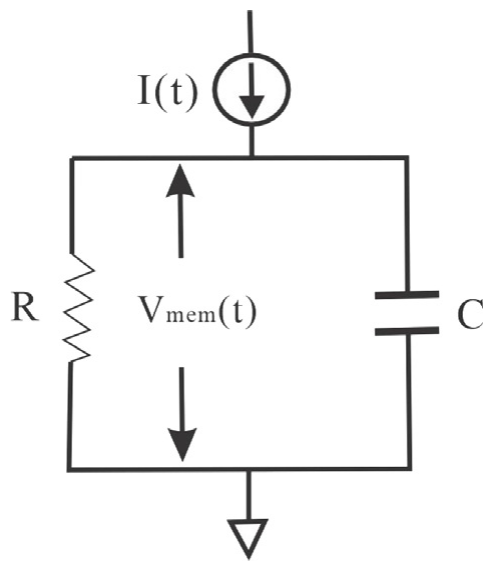
\includegraphics[height=3.8cm, keepaspectratio]{lif_circuit_li2024.png}
    \caption{}
  \end{subfigure}
  \hfill
  \begin{subfigure}[b]{0.64\textwidth}
    \centering
    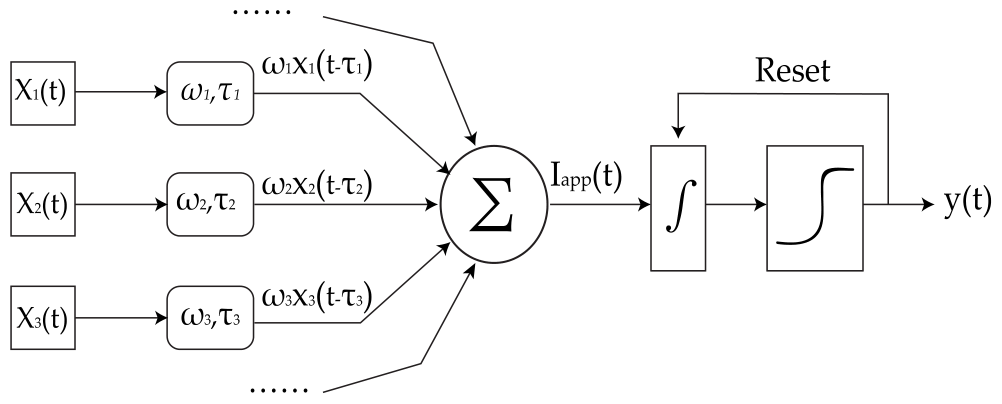
\includegraphics[height=3.8cm, keepaspectratio]{lif_block_li2024.png}
    \caption{}
  \end{subfigure}
  \caption[Principio di funzionamento del modello LIF]{(a) Circuito equivalente RC parallelo del LIF con corrente d'ingresso $I(t)$ e potenziale di membrana $\Vmem(t)$; (b) Schema a blocchi del neurone, da~\cite{li2024}.}
  \label{fig:lif_model}
\end{figure}

Quando la tensione di membrana $\Vmem(t)$ raggiunge la tensione di soglia $\Vthr$, il neurone genera uno spike e la tensione viene riportata subito a un valore inferiore, il potenziale di reset $V_{\mathrm{reset}}$~\cite{li2024} (che nei modelli più semplici coincide con il potenziale di riposo, ma in chip più avanzati come ROLLS può essere regolato separatamente~\cite{qiao2015}). Dopo aver generato uno spike, i neuroni possono rimanere anche inattivi per un breve intervallo di tempo, senza generare un nuovo impulso anche se continua ad arrivare corrente~\cite{indiveri2011, qiao2015}. Entrano in una specie di periodo refrattario. In pratica, aumentando la corrente in ingresso il neurone spara sempre più velocemente (secondo la sua curva caratteristica frequenza/corrente), ma il periodo refrattario fissa comunque una frequenza massima di sparo, che evita consumi eccessivi.

Come abbiamo visto in precedenza, esistono anche altri modelli di LIF più completi, che introducono una seconda variabile:
\begin{itemize}
  \item Il modello di Izhikevich introduce la variabile di recupero $U$. Valgono queste due equazioni:
  \begin{equation}
    \frac{\mathrm{d}\Vmem}{\mathrm{d}t} = 0{,}04\Vmem^2 + 5\Vmem + 140 - U + \Isyn,
    \qquad
    \frac{\mathrm{d}U}{\mathrm{d}t} = a(b\Vmem - U).
    \label{eq:izhikevich}
  \end{equation}
  Nella prima equazione il termine $-U$ agisce come un freno sulla crescita della tensione di membrana. Quando $\Vmem$ sale fino a raggiungere la soglia: il neurone spara l'impulso, la tensione viene riportata al valore di reset e la variabile $U$ aumenta di una certa quantità, frenando temporaneamente l'attività del neurone. Regolando $U$, si riescono a imitare molti comportamenti dei neuroni reali, come il bursting~\cite{indiveri2011, ronchini2023}.
  \item L'AdEx-I\&F invece utilizza una corrente di adattamento al posto di $U$ per frenare il neurone. Il termine quadratico che c'è nel modello di Izhikevich è sostituito da un termine esponenziale, e come vedremo nella Sezione~\ref{subsec:famiglie_neuroni}, si rivela molto utile perché si realizza facilmente sfruttando la fisica dei transistori CMOS sottosoglia~\cite{indiveri2011}.
\end{itemize}

\clearpage

% ==============================================================================
% SEZIONE 2 — APPLICAZIONI BIOMEDICALI DELLE SNN IN SISTEMI IMPIANTABILI
% ==============================================================================
\section[Applicazioni biomedicali impiantabili]{Applicazioni biomedicali delle SNN nei sistemi impiantabili}
\label{sec:applicazioni}

\subsection{Vincoli dei dispositivi impiantabili e ruolo della codifica a spike}
\label{subsec:vincoli_impiantabili}


Progettare un dispositivo elettronico impiantabile è molto più complicato rispetto a un normale dispositivo indossabile, perché ci sono diversi vincoli fisici da rispettare. 

Il primo riguarda il calore generato dal chip. Lavorando a contatto con il tessuto cerebrale, la potenza dissipata deve rimanere bassissima per non surriscaldare il tessuto stesso. Come riferimento, un singolo neurone biologico consuma per la sua attività metabolica circa $0{,}5\text{--}\SI{4{,}0}{\nano\watt}$, una quantità di calore che il nostro corpo riesce a smaltire normalmente~\cite{ronchini2023}. 

A questo si aggiungono i limiti di spazio e di consumo energetico. Nei dispositivi impiantabili è fondamentale tenere bassi sia l'area occupata sia la potenza assorbita, in modo da avere sistemi compatti e far durare il più possibile la batteria~\cite{ronchini2023, wu2026}. Il problema diventa ancora più evidente nelle interfacce neurali moderne, che possono arrivare fino a migliaia di canali di registrazione~\cite{wu2026}: acquisire di continuo tutti questi segnali e inviarli via wireless verso l'esterno consumerebbe troppa energia. Per questo conviene elaborare i segnali direttamente sul chip, riducendo la quantità di dati da trasmettere~\cite{ronchini2023, wu2026}.

Un ultimo vincolo importante riguarda i tempi di risposta, ovvero la latenza. Un esempio concreto è la stimolazione cerebrale profonda (DBS), usata per trattare l'epilessia nei pazienti che non rispondono ai farmaci, circa il 30\% dei casi~\cite{ronchini2023}. Questo tipo di stimolazione può funzionare in due modi, open loop o closed loop. Nei sistemi open loop non c'è alcuna retroazione, quindi il dispositivo invia impulsi elettrici in modo continuo secondo uno schema fisso, senza tenere conto di cosa sta succedendo nel cervello; invece nei sistemi closed loop il dispositivo registra l'attività cerebrale, la analizza e invia lo stimolo elettrico solo quando riconosce i segnali tipici di una crisi~\cite{ronchini2023}. L'approccio closed loop risulta più efficace e ha meno effetti collaterali, perchè interviene solo quando serve, ma per riuscire a intervenire in tempo il dispositivo deve riconoscere la crisi localmente e con una latenza molto bassa, nell'ordine dei millisecondi~\cite{ronchini2023}.

Il primo passo comune a tutte le applicazioni biomedicali basate su SNN è convertire il segnale biologico in una sequenza di spike. Tutti i paper che ho analizzato hanno la stessa idea di fondo: generano uno spike solo quando il segnale sale o scende superando una certa soglia. Ecco come avviene nel dettaglio nei paper:
\begin{itemize}
  \item Step-Forward Encoding (SFE), usato in NET-TEN~\cite{ronchini2023}: lavora sui segnali LFP (cioè i potenziali di campo locale), che sono segnali elettrici registrati direttamente nel tessuto cerebrale. L'algoritmo prende il primo valore del segnale come livello di riferimento (chiamato baseline nel paper) e fissa una soglia, definendo una fascia tra $\text{baseline} - \text{soglia}$ e $\text{baseline} + \text{soglia}$. Per quanto riguarda i campioni successivi, se il segnale esce verso l'alto viene generato uno spike di salita e la baseline sale del valore della soglia; se scende sotto la fascia viene generato uno spike di discesa e la baseline scende della stessa quantità. Finché il segnale resta dentro questa fascia non viene emesso nessuno spike.
  \item Asynchronous Delta Modulation (ADM), integrato sul chip DYNAP-SE2~\cite{bartels2025}: a differenza di SFE (che è eseguito via software), qui generazione di spike avviene tramite un circuito analogico posto subito dopo l'amplificatore del segnale EEG intracranico. Ogni volta che l'ampiezza varia di più di una soglia prefissata, genera uno spike di salita se il segnale sta crescendo, oppure di discesa se sta diminuendo. In questo modo produce molti spike solo quando il segnale varia rapidamente, come durante una crisi, e quasi nessuno nei momenti di quiete.
  \item Analog-to-Spike Converter (ASC), usato in NeuroSEED~\cite{wu2026}: anche in questo caso la generazione avviene in hardware. Due comparatori controllano continuamente se il segnale supera una soglia superiore o scende sotto una soglia inferiore: appena succede, il circuito emette uno spike di salita o di discesa, e tramite un piccolo DAC capacitivo da 1 bit, riporta subito la tensione al livello intermedio di riferimento (così da poter rilevare la variazione successiva senza andare in saturazione). C'è poi un blocco refrattario che aggiunge una breve pausa dopo ogni spike per limitare la frequenza massima di uscita.
  \item Codifica Delta-Sigma, usata con Xylo~\cite{li2024}: viene applicata via software al segnale EEG di scalpo già filtrato. Divide l'escursione di ampiezza del segnale in livelli fissi equidistanti. Ogni volta che il segnale attraversa uno di questi livelli, viene generato uno spike di salita se sta crescendo oppure uno spike di discesa se sta diminuendo. Durante una crisi epilettica, dato che il segnale EEG diventa più ampio e oscilla più velocemente, attraversa molti più livelli e produce quindi una sequenza di spike molto più fitta.
\end{itemize}


\subsection{Rilevamento di eventi epilettici da LFP: NET-TEN (Ronchini et al., 2023)}
\label{subsec:netten_app}

Il chip NET-TEN, presentato da Ronchini et al.\ (2023)~\cite{ronchini2023}, è un esempio di rete neuromorfica pensata per un dispositivo impiantabile. È realizzato interamente con circuiti analogici in tecnologia CMOS \SI{180}{\nano\meter} fatti lavorare in sottosoglia, occupa un'area di \SI{1{,}08}{\milli\meter\squared} ed è alimentato a soli $\Vdd = \SI{250}{\milli\volt}$. Il suo scopo è riconoscere gli eventi epilettici a partire dai potenziali di campo locale (LFP). Rileva sia le crisi vere e proprie (eventi ictali), sia le scariche brevi che possono comparire tra una crisi e l'altra (eventi interictali)~\cite{ronchini2023}.

Per testare il chip, gli autori hanno usato segnali registrati in vitro da 10 fettine di cervello di topo, prese da 10 animali diversi così da includere la variabilità biologica. Le fettine sono state trattate con una sostanza chimica (la 4-aminopiridina, 4AP) che induce attività epilettica, e poi appoggiate su una matrice di elettrodi (MEA $6\times 10$) campionando il segnale LFP a \SI{2}{\kilo\hertz}. Da queste registrazioni sono stati estratti 10 segmenti da \SI{100}{\second}: 9 contengono una crisi ictale (di cui 3 includono anche scariche interictali), mentre uno contiene soltanto un artefatto elettrico, cioè un disturbo non dovuto a una crisi~\cite{ronchini2023}.

Prima di arrivare al chip, questi segnali LFP vengono convertiti in spike via software (in MATLAB) con l'algoritmo SFE visto sopra. Dato che una soglia più bassa genera più spike e una più alta ne genera meno, la soglia viene regolata in modo che circa il 30\% dei campioni totali produca uno spike. Le sequenze digitali così ottenute vengono poi trasformate in impulsi elettrici e inviate ai 10 neuroni d'ingresso di NET-TEN. Cinque ricevono gli spike di salita e gli altri cinque quelli di discesa~\cite{ronchini2023}.


La rete è fatta da 3 strati in cascata, formati da 10 neuroni ciascuno, basati sul modello di Izhikevich. Ogni neurone d'ingresso si collega a due neuroni dello strato intermedio, mentre tra lo strato intermedio e quello di uscita le connessioni sono uno a uno. Ogni collegamento utilizza una sinapsi eccitatoria (EPSC) abbinata a un circuito di plasticità STDP, che regola il peso della sinapsi in base alla distanza temporale tra gli spike dei due neuroni collegati. Anche se tutti i circuiti condividono le stesse tensioni di polarizzazione, dato che stiamo lavorando in sottosoglia, il mismatch comporta che i neuroni non si comportino tutti esattamente allo stesso modo. Misurando tutte e 10 le uscite del chip, solo 4 canali hanno prodotto risultati utili~\cite{ronchini2023}.

I risultati ottenuti su questi 4 canali sono mostrati in figura~\ref{fig:netten_app}. Prima di tutto i consumi sono bassissimi: la potenza statica è di appena \SI{0{,}68}{\pico\watt}, mentre la potenza media durante il rilevamento è di \SI{3{,}50}{\nano\watt}. Come visto prima, si tratta di un valore paragonabile al consumo metabolico di un singolo neurone biologico ($0{,}5\text{--}\SI{4{,}0}{\nano\watt}$), quindi il calore prodotto non rischierebbe di danneggiare il tessuto cerebrale. Inoltre si raggiunge una precisione di 0,998 (quasi nessun falso allarme) e risponde con un ritardo medio di \SI{110{,}4}{\milli\second} per una crisi ictale e di \SI{126{,}6}{\milli\second} per una interictale ~\cite{ronchini2023}.


Gli autori hanno poi provato a capire come distinguere tra crisi ictale, scarica interictale e un semplice artefatto elettrico, e hanno notato che: quando inizia una crisi o una scarica, gli spike iniziali arrivano molto ravvicinati tra loro, mentre con l'artefatto sono molto più distanziati; una crisi ictale produce moltissimi spike (mediana di 1117,5), contro pochissimi per una scarica interictale (mediana di 4,5) e un valore intermedio per l'artefatto (mediana di 27,5). Propongono questa regola: prima si verifica che tra il primo e il terzo spike passino meno di \SI{10}{\milli\second} (scartando così l'artefatto), poi si controlla che nei successivi \SI{190}{\milli\second} arrivino almeno altri 10 spike (distinguendo la crisi vera e propria da una scarica interictale). Questa logica può essere integrata sul chip con due semplici contatori digitali (un contatore temporale che aggiunge appena \SI{31}{\pico\watt} e un piccolo contatore di spike dal consumo trascurabile). La potenza totale è praticamente rimasta invariata, e comunque il ritardo di riconoscimento resta sotto lo 0,6\% della durata mediana di una crisi~\cite{ronchini2023}.

\begin{figure}[tb]
  \centering
  \begin{subfigure}[b]{0.53\textwidth}
    \centering
    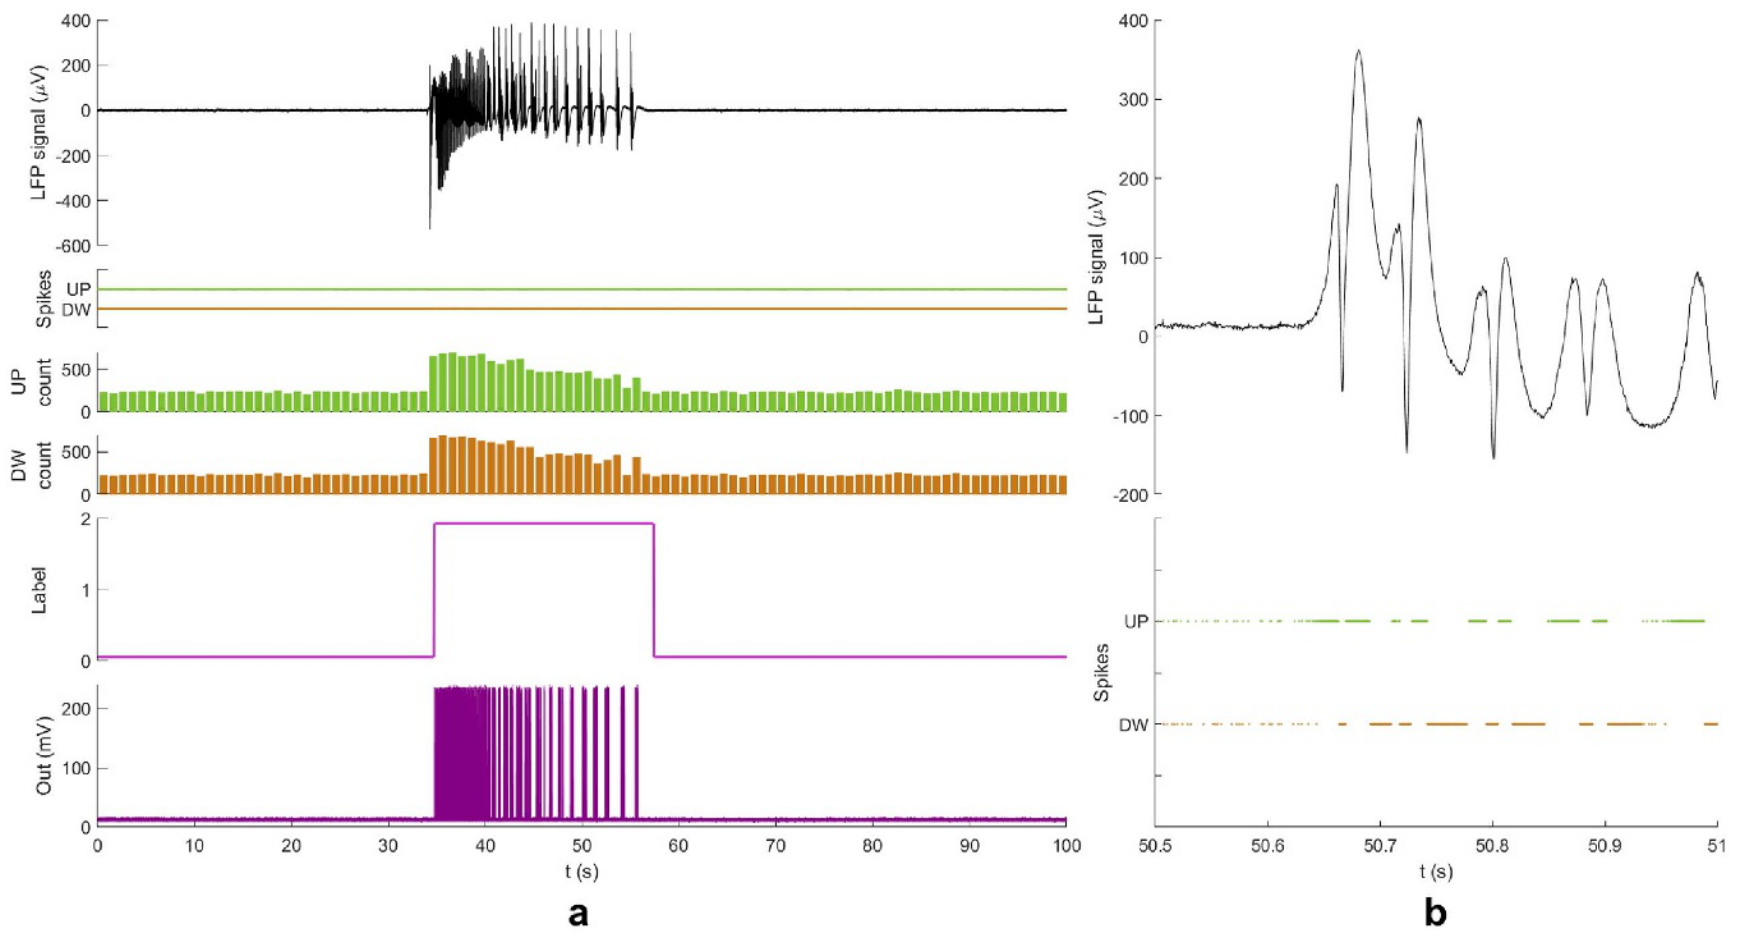
\includegraphics[width=\linewidth]{netten_lfp_detection.png}
    \caption{}
  \end{subfigure}
  \hfill
  \begin{subfigure}[b]{0.45\textwidth}
    \centering
    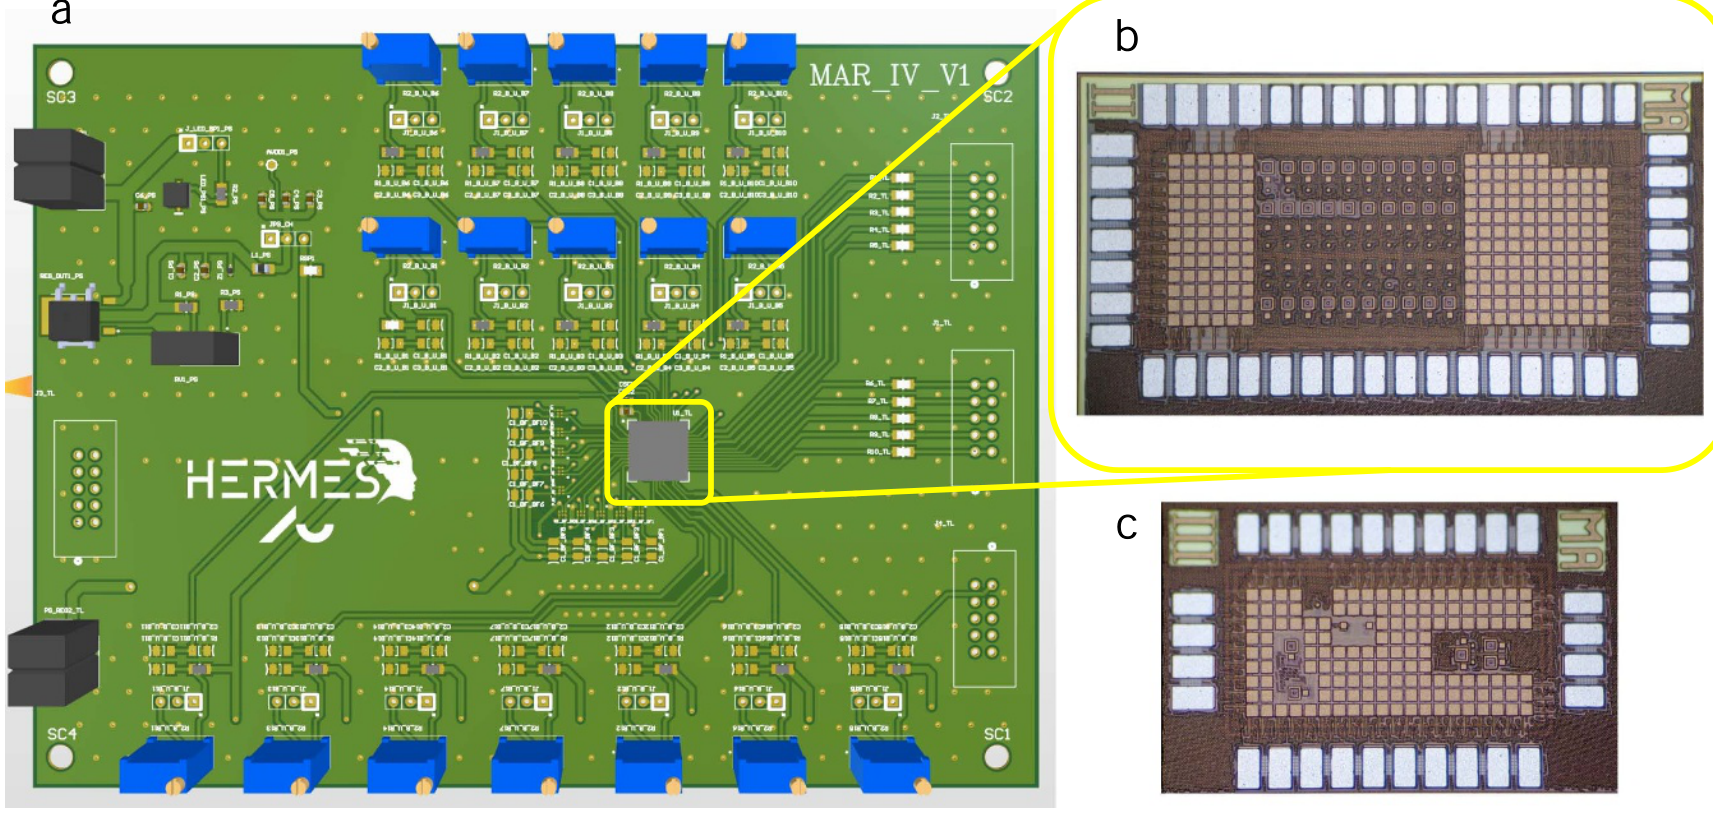
\includegraphics[width=\linewidth]{netten_pcb_die.png}
    \caption{}
  \end{subfigure}
  \caption[Sistema NET-TEN: rilevamento ictale da LFP e die CMOS]{(a) Esempio di tracciato LFP di \SI{100}{\second} di una crisi ictale; (b) PCB usata per la caratterizzazione, con die NET-TEN ~\cite{ronchini2023}}
  \label{fig:netten_app}
\end{figure}

Nel paper vengono tuttavia mostrati i limiti di questo prototipo: l'acquizione, il filtraggio e la codifica SFE avvengono via software, fuori dal chip; le tensioni di bias sono regolate manualmente tramite potenziometri, e i condensatori STDP utilizzati trattengono i pesi solo per tempi nell'ordine di decine di millisecondi, quindi non c'è apprendimento permanente~\cite{ronchini2023}.

\subsection{Un sistema impiantabile completo: NeuroSEED (Wu et al., 2026)}
\label{subsec:neuroseed_app}

Nel paper di Wu et al.\ (2026)~\cite{wu2026} si affronta il problema di realizzare un sistema neurale impiantabile completo su un singolo chip. Il sistema si chiama NeuroSEED: è realizzato in tecnologia CMOS \SI{40}{\nano\meter}, è alimentato a \SI{1{,}2}{\volt} e occupa un'area totale di \SI{0{,}70}{\milli\meter\squared}. Gestisce 32 canali per rilevare i potenziali d'azione (in banda fino a \SI{5{,}2}{\kilo\hertz}) e trasmetterli via wireless verso l'esterno. NeuroSEED è organizzato in quattro blocchi principali, mostrati in figura~\ref{fig:neuroseed_arch}.

Il primo blocco è lo stadio di acquisizione analogico di 32 canali. Il chip usa un solo amplificatore a basso rumore condiviso tra i 32 elettrodi tramite una serie di interruttori che leggono i canali a turno (tecnica chiamata multiplexing nel tempo, TDM). Ogni canale viene così campionato a \SI{10{,}4}{\kilo\hertz}, una frequenza sufficiente per rilevare i potenziali d'azione senza sprecare energia con frequenze più alte. Condividere l'amplificatore riduce drasticamente l'area di ingresso a soli \SI{0{,}0032}{\milli\meter\squared} per canale, mantenendo un rumore molto basso (\SI{2{,}9}{\micro\volt\textsubscript{rms}}) e un guadagno regolabile tra \SI{41{,}2}{\decibel} e \SI{58{,}3}{\decibel} per compensare le variazioni dell'impedenza degli elettrodi nel tempo~\cite{wu2026}.

Il secondo blocco serve a cancellare l'offset DC che si crea all'interfaccia tra elettrodo e tessuto biologico, che può arrivare fino a $\pm\SI{50}{\milli\volt}$. C'è un anello di controllo digitale che ogni \SI{4{,}8}{\second} esegue una calibrazione da \SI{0{,}96}{\milli\second}. Misura l'offset medio sfruttando gli spike del convertitore ASC (descritto nella Sezione~\ref{subsec:vincoli_impiantabili}), lo accumula in un contatore a 6 bit e applica all'ingresso una tensione uguale e opposta tramite un DAC capacitivo a 6 bit~\cite{wu2026}.

Il terzo blocco riguarda la conversione in spike e il riconoscimento dei potenziali d'azione. Dopo la parte di amplificazione, il segnale viene di nuovo separato nei 32 canali, ciascuno dotato del convertitore ASC e di un piccolo rivelatore asincrono senza clock, che quindi consuma solo quando arrivano eventi. Il rivelatore capisce qual'è il minimo del segnale e da lì conta quanti spike di salita arrivano fino al picco successivo. Questo conteggio misura di quanto si è alzato il segnale dal punto più basso al punto più alto, e se la salita supera una soglia programmabile, il circuito riconosce un potenziale d'azione vero e proprio, filtrando così le oscillazioni del rumore di fondo. Questo blocco occupa \SI{0{,}0007}{\milli\meter\squared} e consuma \SI{0{,}48}{\micro\watt} per canale~\cite{wu2026}.

L'ultimo blocco è il trasmettitore wireless. Il fatto di riconoscere i potenziali d'azione direttamente sul chip riduce notevolmente il volume di dati da inviare all'esterno. Il trasmettitore integrato (IR-UWB, a \SI{4{,}25}{\giga\hertz}) si accende solo quando viene riconosciuto un potenziale d'azione. In questo modo il suo consumo medio scende a \SI{4{,}6}{\micro\watt} totali~\cite{wu2026}.

% --- FIGURA 2.3: Diagramma a blocchi NeuroSEED (da Wu et al., 2026) ---
\begin{figure}[tb]
  \centering
  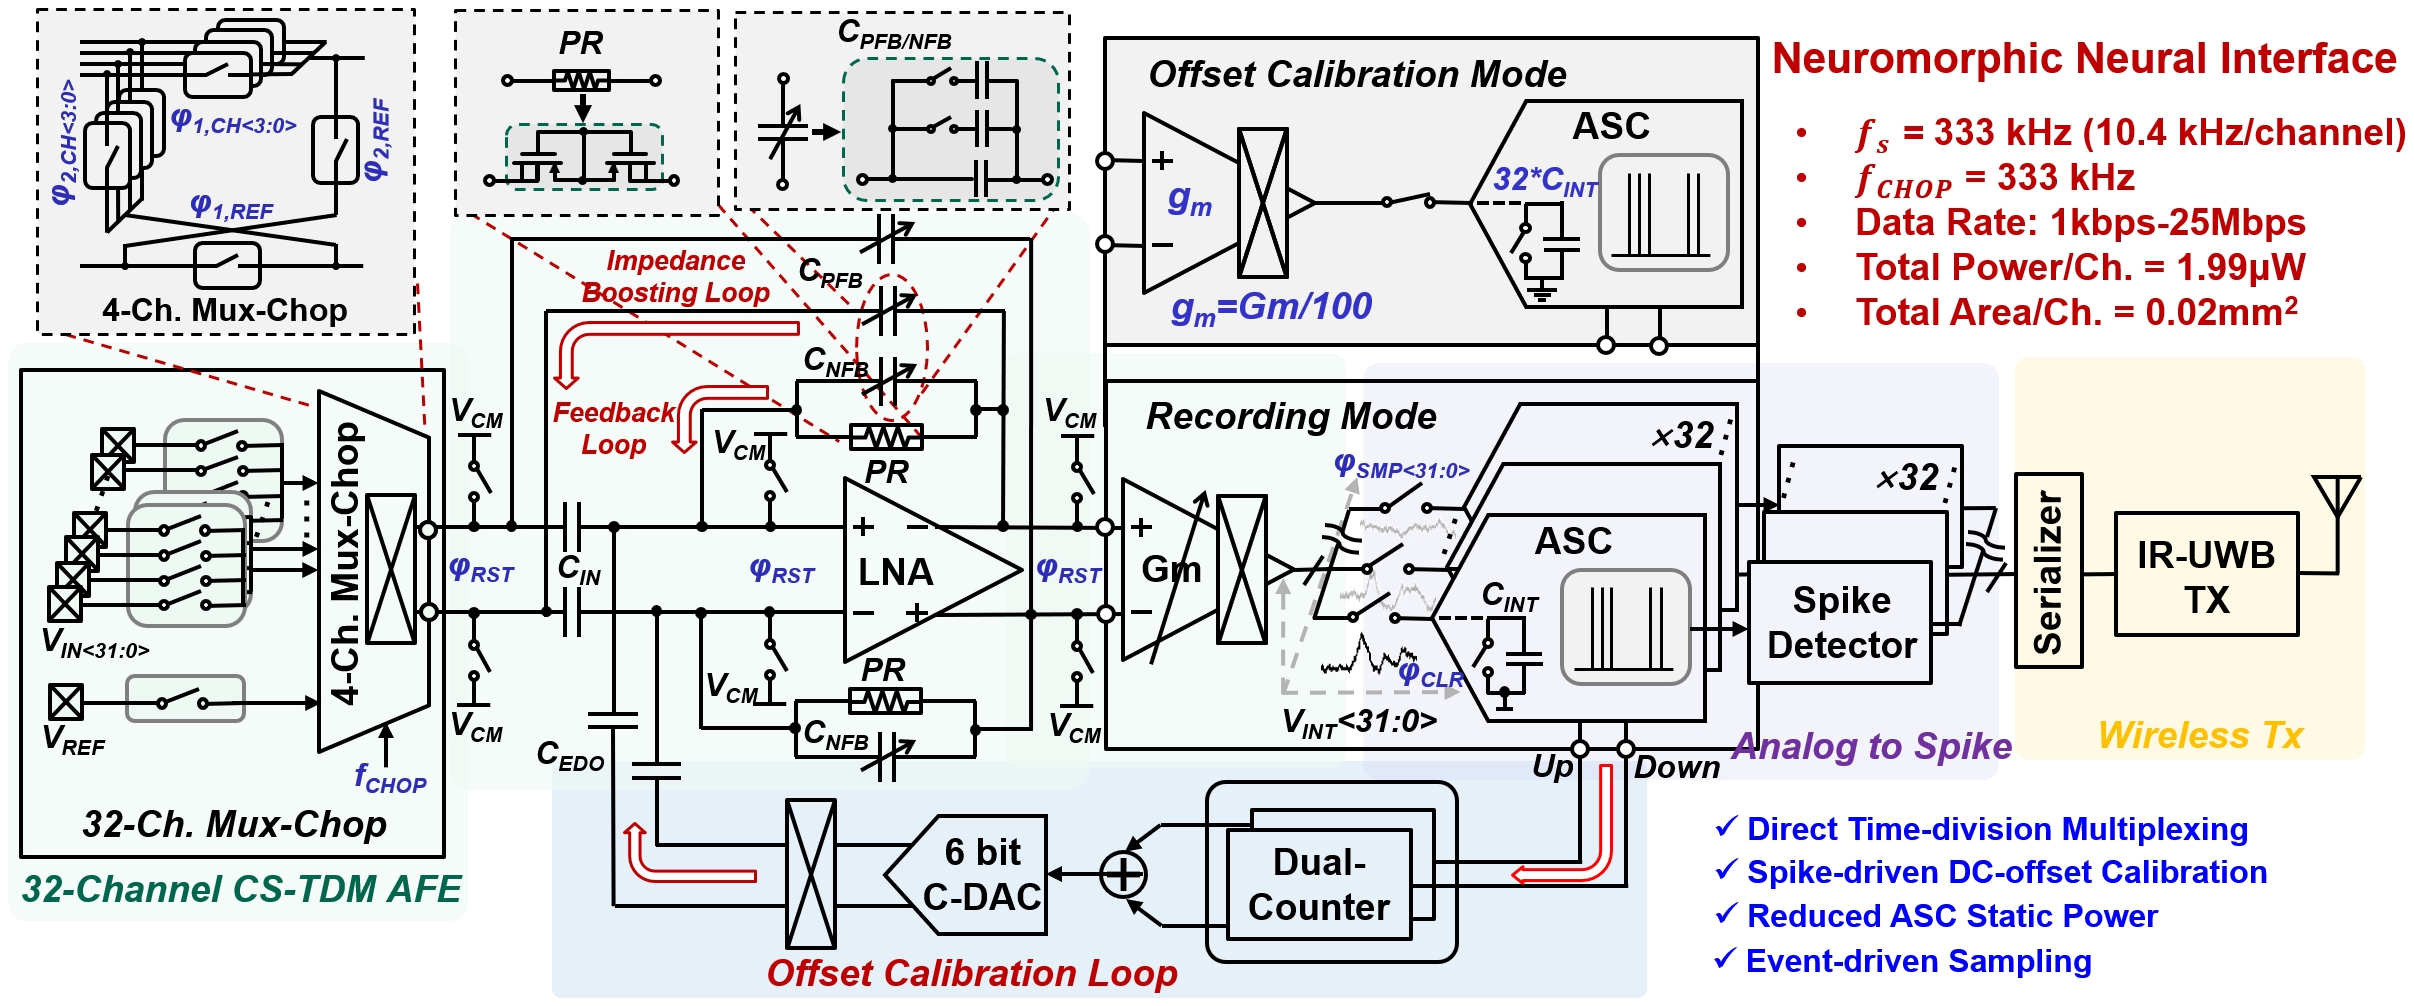
\includegraphics[width=\textwidth]{neuroseed_arch.png}
  \caption[Architettura del chip NeuroSEED]{Architettura del chip NeuroSEED~\cite{wu2026}.}
  \label{fig:neuroseed_arch}
\end{figure}

Il chip, mostrato in figura~\ref{fig:neuroseed_silicio}a, consuma nel complesso \SI{63{,}61}{\micro\watt}, pari a \SI{1{,}99}{\micro\watt} per canale. Come si vede in figura~\ref{fig:neuroseed_silicio}b, è stato testato su dei dati registrati in vivo su ratto e riesce a tracciare in modo affidabile i potenziali d'azione riducendo drasticamente i dati da trasmettere~\cite{wu2026}.

\begin{figure}[tb]
  \centering
  \begin{subfigure}[b]{0.52\textwidth}
    \centering
    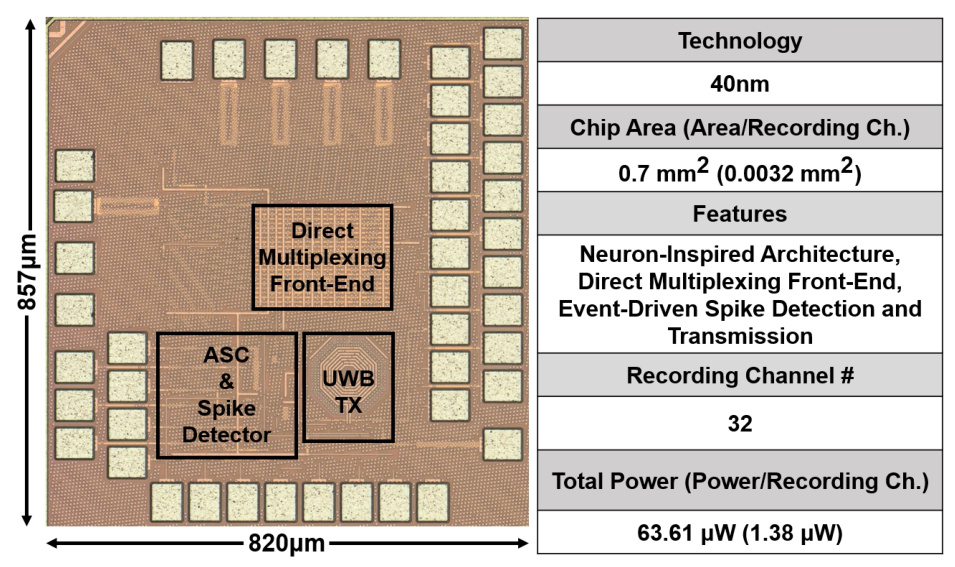
\includegraphics[width=\linewidth]{neuroseed_die.png}
    \caption{}
  \end{subfigure}
  \hfill
  \begin{subfigure}[b]{0.44\textwidth}
    \centering
    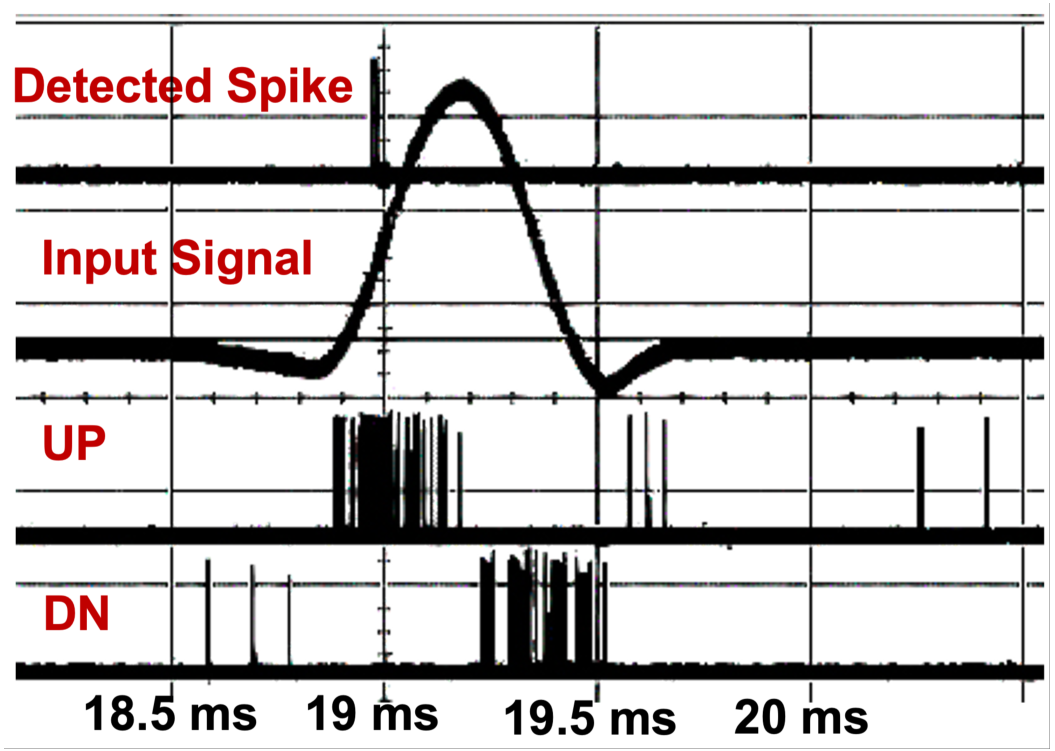
\includegraphics[width=\linewidth]{neuroseed_invivo.png}
    \caption{}
  \end{subfigure}
  \caption[Die CMOS e misura \emph{in vivo} di NeuroSEED]{(a) Die del NeuroSEED e riepilogo prestazioni; (b) Tracciato sperimentale ed eventi \texttt{UP}/\texttt{DN} dell'ASC~\cite{wu2026}.}
  \label{fig:neuroseed_silicio}
\end{figure}

\newpage

\subsection{Rilevamento di crisi epilettiche da iEEG: DYNAP-SE2 (Bartels et al., 2025)}
\label{subsec:dynapse2_app}

Nel paper di Bartels et al.\ (2025)~\cite{bartels2025} il rilevamento delle crisi epilettiche viene testato su segnali registrati sull'uomo, usando il processore neuromorfico mixed-signal DYNAP-SE2. Il chip è CMOS \SI{180}{\nano\meter}, con parti sia analogiche che digitali. Lavora in tempo reale senza un clock globale. Al suo interno ospita 4 core da 256 neuroni analogici AdEx-I\&F ciascuno. Integra sullo stesso die anche il circuito per l'acquisizione e per la codifica ADM già descritto nella sezione~\ref{subsec:vincoli_impiantabili}~\cite{bartels2025}.

Per testare il sistema, gli autori hanno usato i dati di un EEG intracranico (iEEG) del dataset pubblico SWEC-ETHZ. Hanno selezionato 5 pazienti con 2 crisi ciascuno, quindi un totale di 10 crisi. I segnali digitali del dataset sono stati convertiti in forma analogica con un DAC esterno e inviati all'AFE integrato, dove il circuito ADM li trasforma in sequenze di spike~\cite{bartels2025}.

Dato che i circuiti analogici in sottosoglia di DYNAP-SE2 hanno un mismatch piuttosto alto (tra il 20\% e il 30\% sui parametri di polarizzazione) e pesi a bassa precisione, gli autori costruiscono una rete molto semplice, formata da soli due strati di neuroni in cascata con pesi fissi. Il funzionamento si basa sui tempi di risposta delle sinapsi e su come i neuroni sono collegati tra loro. Il primo strato, chiamato strato di traduzione, riceve gli spike dall'ADM e usa tre tipi di neuroni (eccitatori ricorrenti R-E, inibitori ricorrenti R-I e inibitori rapidi FF-I) per bloccare i segnali troppo lenti o troppo veloci e lascia passare solo le frequenze tra \SI{200}{\hertz} e \SI{600}{\hertz}. Il secondo strato, chiamato NLNG (Non-Local Non-Global), collega tra di loro i neuroni usando sinapsi a peso costante. Quando più canali vicini si attivano insieme durante una crisi, i neuroni di quella zona iniziano a sparare molto più velocemente e formano gruppi sincronizzati, come si vede in figura~\ref{fig:dynapse2_sync}~\cite{bartels2025}.

\begin{figure}[tb]
  \centering
  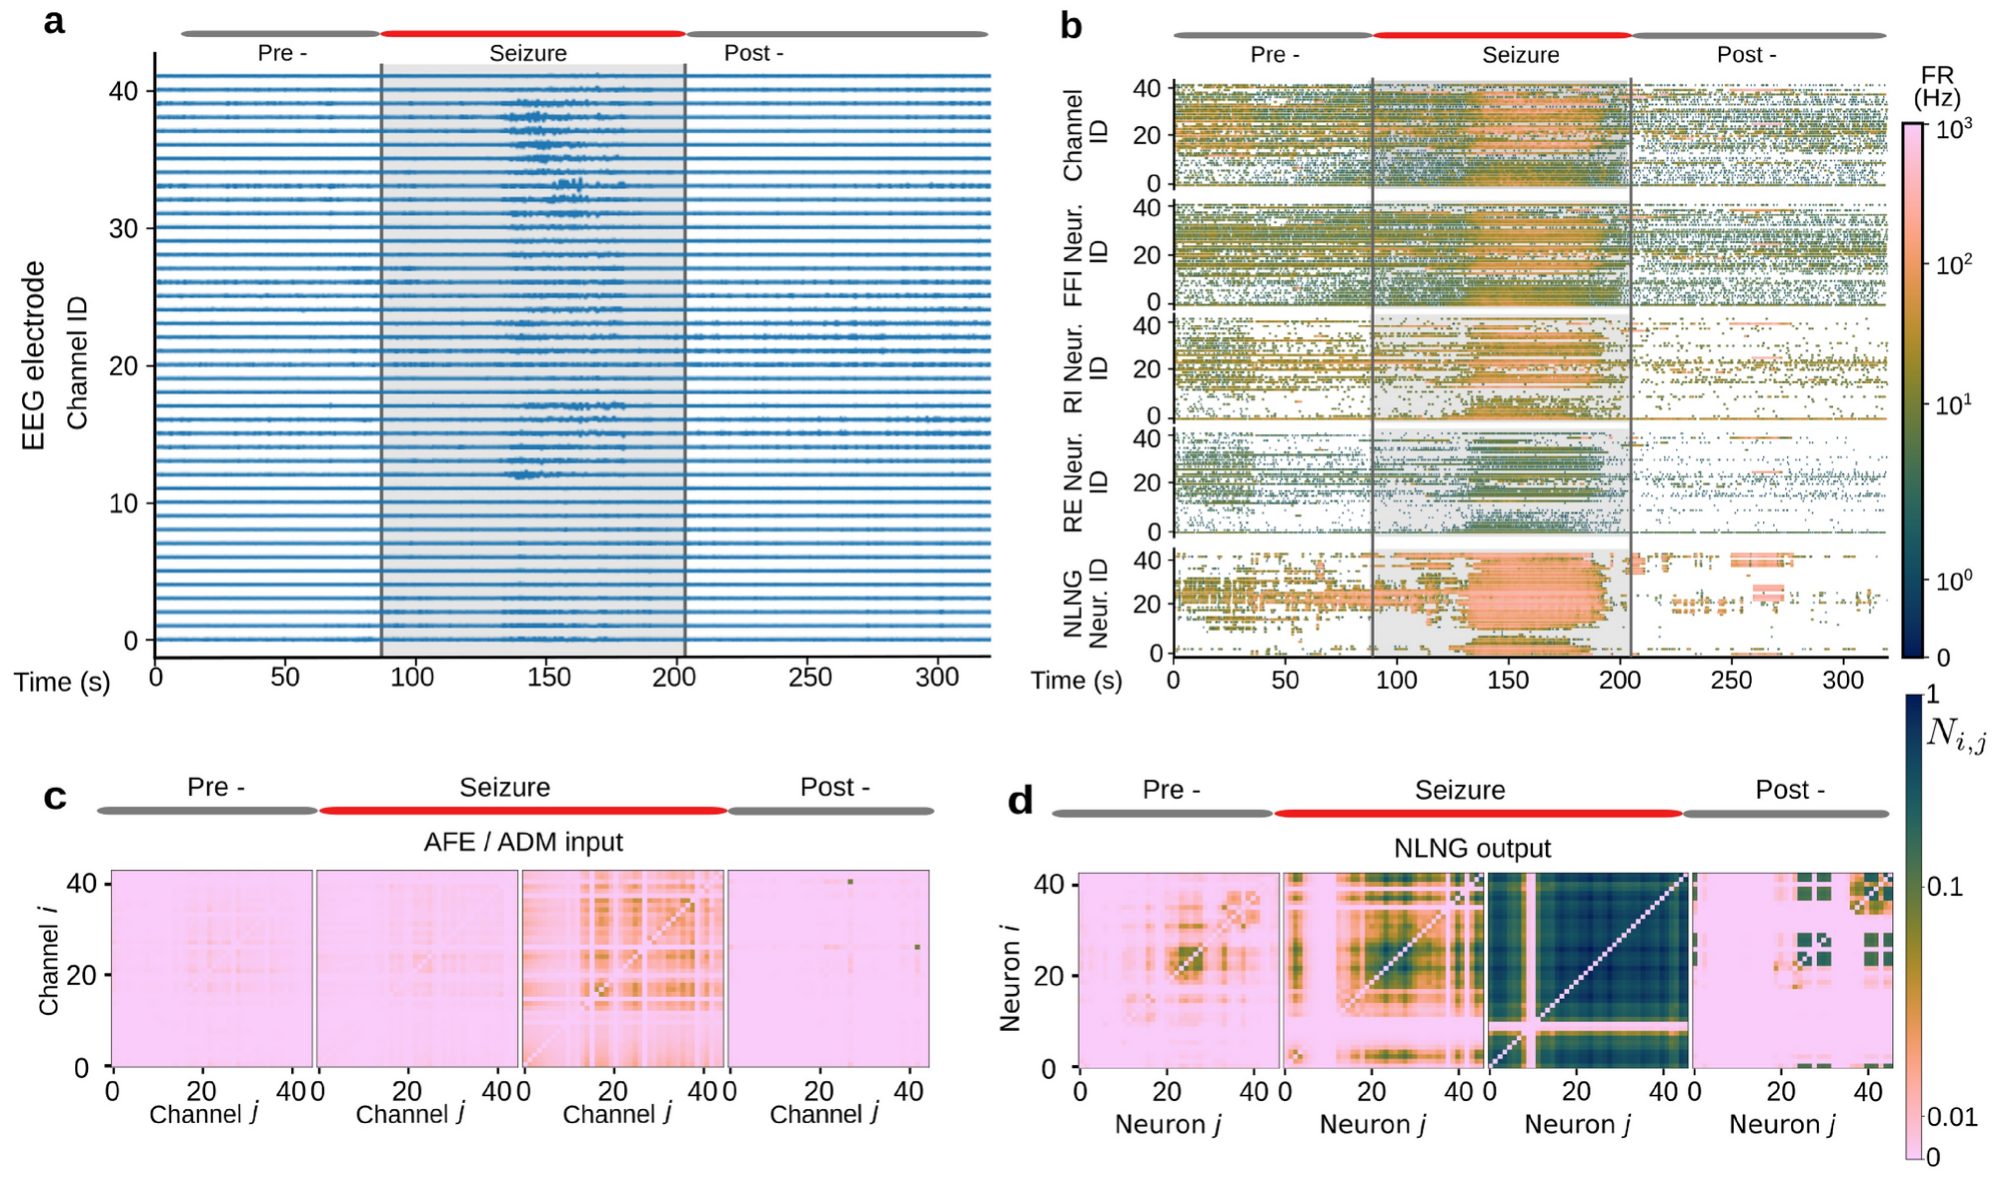
\includegraphics[width=0.96\textwidth]{dynapse2_sync.png}
  \caption[Rilevamento di crisi epilettiche su iEEG umano con DYNAP-SE2]{Elaborazione di 42 canali iEEG (Paziente 1, Crisi 1 del dataset SWEC-ETHZ) su DYNAP-SE2~\cite{bartels2025}: (a) tracciati iEEG con il periodo di crisi evidenziato; (b) sequenze di spike dall'ADM fino allo strato NLNG; (c--d) matrici di sincronizzazione tra canali in ingresso (AFE/ADM) e in uscita (NLNG) prima, durante e dopo la crisi.}
  \label{fig:dynapse2_sync}
\end{figure}

Quindi dallo strato NLNG escono degli spike. Per capire se questi spike sono effettivamente riconducibili ad una crisi, gli autori usano fuori dal chip un classificatore lineare (Linear SVM). Gli spike in uscita vengono divisi in finestre da \SI{1}{\second} e si calcola la frequenza di sparo dei neuroni in ogni finestra. In media sui 5 pazienti si ottiene un'accuratezza del 78,35\% (percentuale totale di finestre classificate correttamente), una sensibilità del 66,71\% (crisi riconosciute), una specificità dell'85,54\% (periodi senza crisi riconosciuti correttamente) e un'AUC dell'80,91\% (indice che riassume il compromesso tra sensibilità e falsi positivi). Gli autori hanno poi confrontato questo risultato dando al classificatore direttamente gli spike dell'ADM senza passare dalla SNN: la rete migliora soprattutto il riconoscimento delle crisi (la sensibilità sale dal 58,56\% al 66,71\%), mentre l'ADM da solo ha una specificità leggermente più alta (89,55\%), cioè riconosce un po' meglio i momenti senza crisi~\cite{bartels2025}.

Per quanto riguarda i consumi, la potenza media stimata a \SI{1{,}8}{\volt} è di circa \SI{150}{\micro\watt}, pari a \SI{2{,}8}{\micro\watt} per canale\cite{bartels2025}.

\subsection{Rilevamento di crisi epilettiche da EEG di scalpo: Xylo (Li et al., 2024)}
\label{subsec:xylo_app}

Nel paper di Li et al.\ (2024)~\cite{li2024} si ua il processore neuromorfico Xylo per riconoscere le crisi epilettiche in tempo reale a partire da registrazioni di EEG di scalpo, cioè acquisite in modo non invasivo con elettrodi sulla testa. Xylo è un processore SNN interamente digitale in tecnologia CMOS \SI{28}{\nano\meter}, occupa \SI{6{,}5}{\milli\meter\squared} e dispone di \SI{124}{\kilo\byte} di memoria SRAM. Può gestire fino a 1000 neuroni LIF digitali (più 8 neuroni di uscita) con pesi a 8 bit. La rete viene prima addestrata via software fuori dal chip e poi i suoi parametri vengono caricati su Xylo~\cite{li2024}.

Gli autori hanno testato il sistema su due dataset pubblici di EEG di scalpo. Prima di arrivare al chip, è stato fatto del filtraggio via software per togliere artefatti come battito cardiaco e movimenti muscolari. Il segnale filtrato viene poi convertito in spike con la codifica Delta-Sigma descritta nella sezione~\ref{subsec:vincoli_impiantabili}~\cite{li2024}.

La rete utilizzata si chiama WaveSense ed è una SNN feed-forward formata da più blocchi in cascata che sfruttano sinapsi con diverse costanti di tempo. Richiede solo 2400 pesi, molti meno rispetto alle reti neurali tradizionali confrontate nel paper, che arrivano anche a diversi milioni di parametri. La rete viene addestrata fuori dal chip con l'algoritmo BPTT (Backpropagation Through Time)~\cite{li2024}.

In simulazione software la rete raggiunge un'accuratezza del 93,3\%. Sul chip invece l'accuratezza scende leggermente all'89,87\%. Su segmenti da \SI{5}{\second}, il ritardo mediano di rilevamento misurato su Xylo è di \SI{0{,}5}{\second}. Per quanto riguarda i consumi, il totale è di \SI{375{,}3}{\micro\watt}, molto più basso rispetto alle soluzioni convenzionali su FPGA confrontate nello studio, che consumano tra \SI{159{,}7}{\milli\watt} e \SI{284}{\milli\watt}~\cite{li2024}. 

Anche per questo esempio, molte fasi come il filtraggio e la codifica Delta-Sigma avvengono fuori dal chip. Inoltre, come osservano gli autori del paper, l'accuratezza resta un po' più bassa rispetto a quella delle reti neurali artificiali tradizionali più grandi~\cite{li2024}.

\subsection{Conclusioni sui pro e contro delle SNN}
\label{subsec:risposta_domanda1}


Quindi, perché usare una SNN in un dispositivo biomedicale impiantabile e quali vantaggi offre rispetto all'elaborazione digitale convenzionale?

Il funzionamento a eventi di una SNN si adatta bene alla natura dei segnali biologici, che sono lenti e passano gran parte del tempo in condizioni normali, cioè gli eventi rilevanti sono concentrati solo in alcuni momenti. Una SNN si attiva solo quando il segnale varia in modo significativo. Un sistema digitale convenzionale invece continua a processare ad ogni ciclo di clock, sprecando energia anche quando non sta succedendo nulla~\cite{ronchini2023, bartels2025, wu2026}.

Per quanto riguarda i consumi, come ho analizzato nella sezione~\ref{subsec:vincoli_impiantabili}, nei lunghi periodi di calma, le tecniche di codifica in spike (tipo ADM o ASC) generano pochissimi impulsi e la rete rimane quasi inattiva, evitando i consumi continui di un clock digitale~\cite{bartels2025, wu2026}. Per esempio, nel caso di NET-TEN, la sola parte di elaborazione, cioè una piccola rete analogica in sottosoglia, consuma appena \SI{3{,}50}{\nano\watt} (paragonabili a un singolo neurone biologico)~\cite{ronchini2023}. Con il processore mixed-signal DYNAP-SE2 si stimano circa \SI{150}{\micro\watt} (\SI{2{,}8}{\micro\watt} per canale)~\cite{bartels2025}. E anche un chip SNN interamente digitale come Xylo si ferma a \SI{375{,}3}{\micro\watt} totali, molto al di sotto delle soluzioni convenzionali su FPGA confrontate nel paper, che arrivano a consumare tra \SI{159{,}7}{\milli\watt} e \SI{284}{\milli\watt}~\cite{li2024}.

Per quanto riguarda la latenza, è molto importante affinché un sistema riconosca e risponda ad una crisi in tempo~\cite{ronchini2023}. Rispetto ai sistemi tradizionali che accumulano prima grandi blocchi di segnale in memoria, le SNN elaborano i dati in tempo reale mentre arrivano, sfruttando circuiti con costanti di tempo paragonabili a quelle dei segnali biologici~\cite{ronchini2023, bartels2025, li2024}. NET-TEN risponde in media in \SI{110{,}4}{\milli\second} a una crisi ictale~\cite{ronchini2023}. Xylo rileva le crisi con un ritardo mediano di \SI{0{,}5}{\second} su segmenti da \SI{5}{\second}~\cite{li2024}. Stiamo parlando di tempi decisamente più bassi rispetto ad altre soluzioni convenzionali confrontate nei paper, che arrivano anche a diversi secondi~\cite{ronchini2023}.

Poi c'è la possibilità di elaborare i segnali localmente sul chip, vicino agli elettrodi. Nei dispositivi convenzionali con anche migliaia di canali, trasmettere continuamente via wireless tutti i segnali grezzi consuma troppa energia~\cite{ronchini2023, wu2026}. Grazie all'estrazione direttamente sul chip dei soli eventi utili (come i potenziali d'azione o l'inizio di una crisi), si riduce il volume di dati da inviare all'esterno. In NeuroSEED il trasmettitore wireless consuma in media solo \SI{4{,}6}{\micro\watt} totali (su \SI{63{,}61}{\micro\watt} dell'intero chip a 32 canali)~\cite{wu2026}.

Quindi complessivamente le SNN offrono un vantaggio concreto nei dispositivi impiantabili perché danno bassi consumi, tempi di risposta ridotti ed elaborazione locale. Restano però alcuni limiti emersi nei vari paper. In quasi tutti i prototipi visti, alcune fasi come l'acquisizione, il filtraggio e la codifica in spike avvengono ancora fuori dal chip, quindi i consumi riportati riguardano solo una parte dell'intero sistema. Inoltre c'è il problema del mismatch nei circuiti in sottosoglia (che ad esempio in NET-TEN rende utili solo 4 canali su 10), e l'accuratezza che resta un po' più bassa rispetto alle reti neurali tadizionali più grandi~\cite{ronchini2023, bartels2025, li2024, wu2026}.

\clearpage

% ==============================================================================
% SEZIONE 3 — IMPLEMENTAZIONI CIRCUITALI CMOS DI NEURONI E PROCESSORI SPIKING
% ==============================================================================
\section[Implementazioni circuitali CMOS]{Implementazioni circuitali CMOS di neuroni e architetture neuromorfiche}
\label{sec:cmos}

\subsection{Stili progettuali e tassonomia dei neuroni in silicio}
\label{subsec:tassonomia_cmos}

Per realizzare un neurone in CMOS, esistono varie soluzioni. Come spiegato in Indiveri et al.\ (2011)~\cite{indiveri2011}, la scelta dipende dall'obiettivo e richiede sempre un compromesso tra consumo energetico, area, precisione, velocità e livello di somiglianza con il neurone biologico~\cite{indiveri2011}.

Generalmente un neurone è composto da più blocchi funzionali. Per costruire questi blocchi si possono seguire diversi stili progettuali~\cite{indiveri2011}. Prima di tutto i segnali interni possono essere rappresentati come tensioni oppure come correnti. Poi il circuito può lavorare a tempo continuo senza clock, oppure a tempo discreto tramite capacità commutate. I transistori MOSFET possono lavorare in sottosoglia oppure in inversione forte. Inoltre i circuiti possono operare con costanti di tempo simili a quelle biologiche, quindi si dice che lavorano in tempo reale, oppure molto più velocemente~\cite{indiveri2011}.

Per i dispositivi biomedicali impiantabili, il regime di sottosoglia offre molti vantaggi~\cite{indiveri2011}. In questa regione la corrente del transistor dipende in modo esponenziale dalla tensione tra gate e source:
\begin{equation}
  I_D = I_0 \exp\!\left(\frac{\kappa V_{\mathrm{GS}}}{\UT}\right),
  \label{eq:subthreshold}
\end{equation}
Questo regime permette di lavorare con correnti piccolissime (fino ai picoampere o femtoampere~\cite{indiveri2011}) e di ottenere costanti di tempo simili a quelle biologiche ($\tau = \Cmem \UT / (\kappa I_\tau)$~\cite{bartels2025}) usando condensatori integrati molto piccoli. Per esempio, in CMOS \SI{180}{\nano\meter} basta un condensatore da \SI{1}{\pico\farad} per ottenere costanti di tempo dell'ordine delle decine di millisecondi~\cite{indiveri2011, qiao2015}.

Se invece si fanno lavorare i transistor in forte inversione, abbiamo meno mismatch, ma le correnti aumentano e le resistenze equivalenti si abbassano drasticamente~\cite{indiveri2011}. Per avere costanti di tempo biologiche servirebbero grossi condensatori esterni al chip~\cite{indiveri2011}. Ovviamente per il sottosoglia c'è il problema del mismatch, quindi generalmente devono essere inclusi dei meccanismi di calibrazione e adattamento~\cite{indiveri2011, qiao2015}.

\subsection{Blocchi circuitali e realizzazione del neurone in CMOS}
\label{subsec:blocchi_fondamentali}

\subsubsection{Integrazione temporale e circuiti log-domain}
Come spiegato nel paper di Indiveri et al.\ (2011)~\cite{indiveri2011}, in un neurone il segnale attraversa due stadi in cascata. Prima le sinapsi ricevono gli spike di tensione provenienti dagli altri neuroni e li trasformano in correnti (eccitatorie EPSC o inibitorie IPSC) che salgono e poi si spengono lentamente. Poi il soma riceve in ingresso queste correnti, le accumula sulla membrana e quando viene superata una soglia genera in uscita un nuovo spike. 

Ci servono quindi dei circuiti che facciano disperdere gradualmente una carica accumulata e che trasformino gli spike di tensione in arrivo in una corrente che varia nel tempo. Come mostrato in Indiveri et al.\ (2011)~\cite{indiveri2011}, sia la perdita passiva della membrana sia la dinamica delle sinapsi si possono descrivere con una semplice equazione differenziale del primo ordine del tipo $\tau \frac{\mathrm{d}y}{\mathrm{d}t} = -y + x$, dove $x$ è il segnale di ingresso, $y$ è l'uscita (una tensione o una corrente) e $\tau$ è la costante di tempo di ritorno a riposo.

Per realizzare questa dinamica in sottosoglia si può lavorare in modalità tensione oppure in modalità corrente~\cite{indiveri2011}. In modalità tensione, il segnale $y$ che ci interessa leggere è la tensione ai capi di un condensatore (come $\Vmem$ nel modello RC visto nella Sezione~\ref{sec:introduzione}). Una soluzione classica di questo tipo è il circuito follower-integrator, usato per modellare la perdita passiva della membrana. Si realizza con un amplificatore a transconduttanza collegato in retroazione negativa a un condensatore, dove l'amplificatore fa da resistenza regolabile che scarica lentamente la capacità~\cite{indiveri2011}. Invece in modalità corrente il segnale di uscita è ad esempio la corrente sinaptica $\Isyn$, oppure la corrente $\Imem$ usata al posto di $\Vmem$~\cite{indiveri2011}. In sottosoglia questo si ottiene con i circuiti log-domain: dato che la corrente di un MOSFET in sottosoglia dipende in modo esponenziale dalla tensione gate-source come visto nell'equazione~\eqref{eq:subthreshold}, la tensione sul condensatore è legata al logaritmo della corrente; combinando quindi un condensatore con reti di transistori in sottosoglia si riescono a integrare gli impulsi nel tempo direttamente in corrente~\cite{indiveri2011}.

% --- FIGURA 3.1: Blocchi integratori log-domain (da Indiveri et al., 2011, Fig. 1) ---
\begin{figure}[tb]
  \centering
  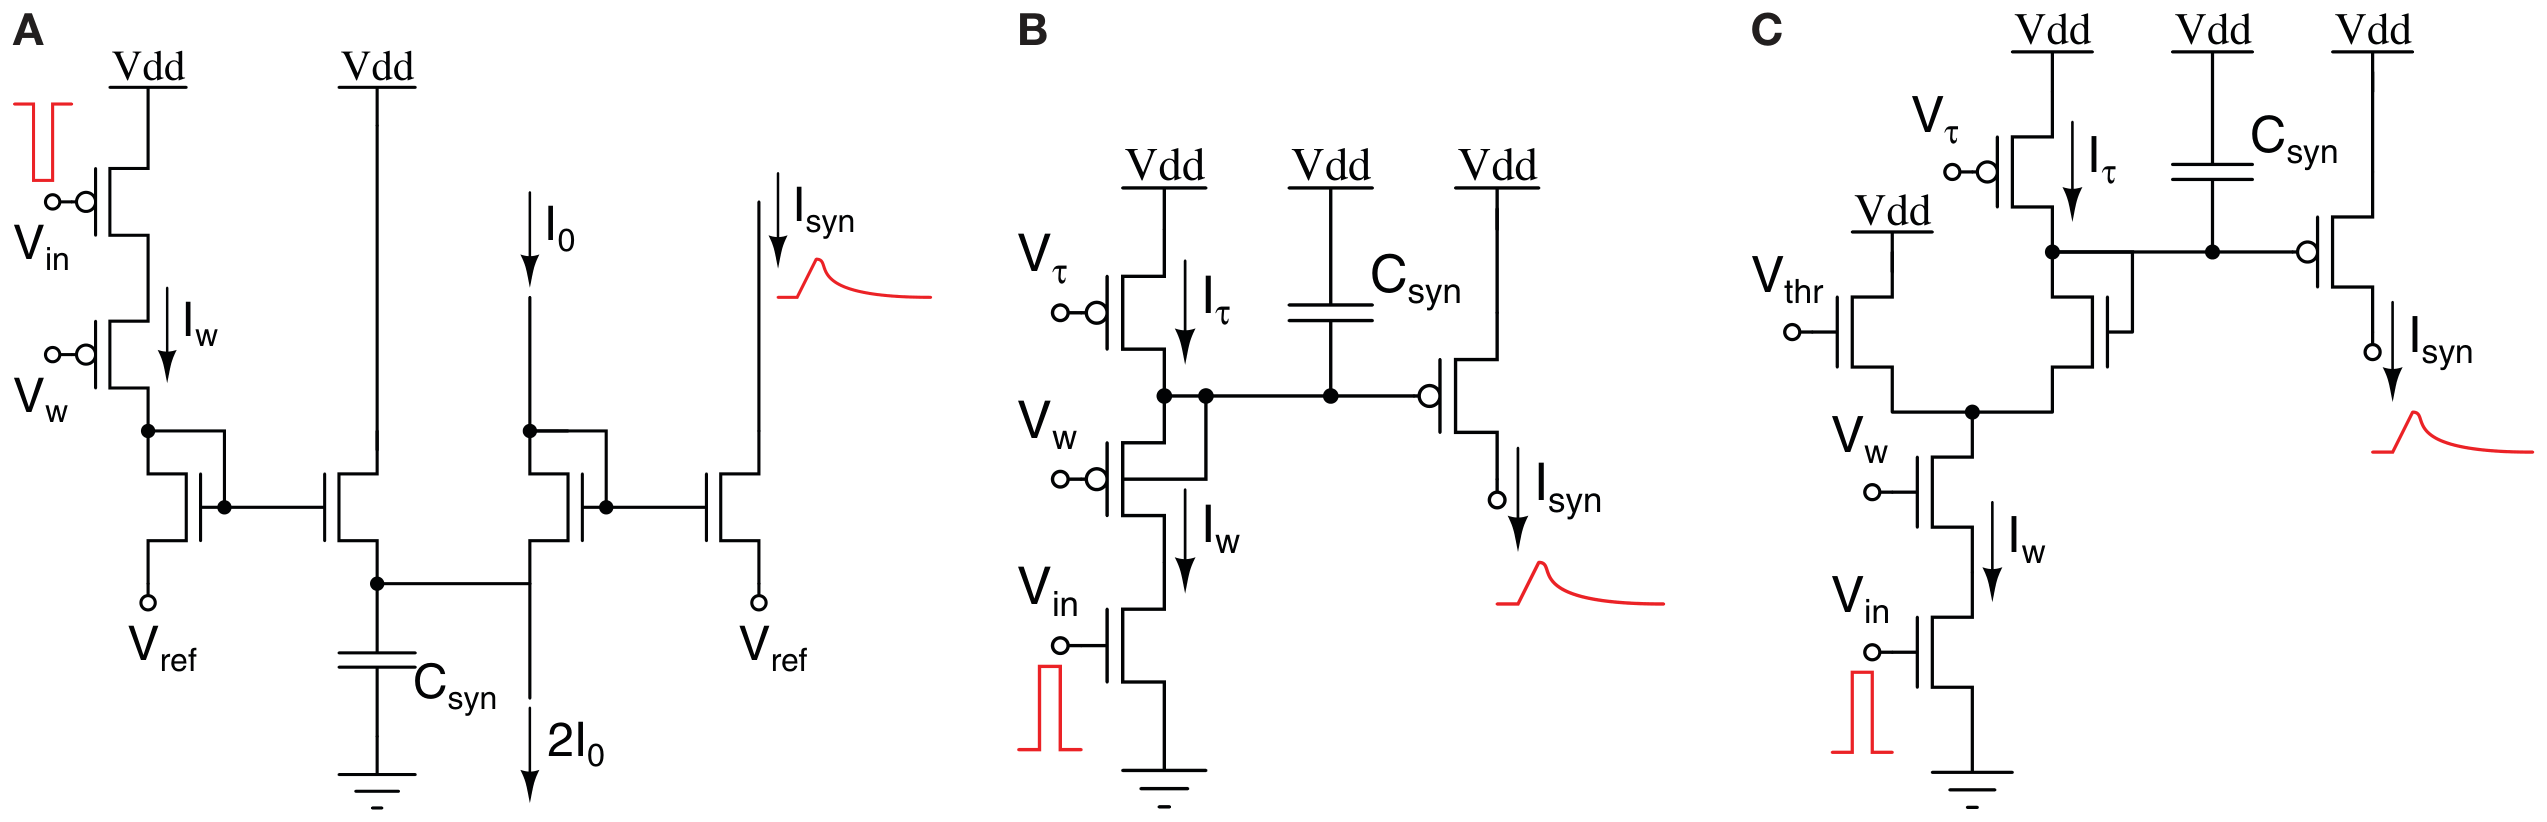
\includegraphics[width=0.98\textwidth]{indiveri_log_domain.png}
  \caption[Circuiti integratori log-domain in sottosoglia]{Circuiti integratori log-domain in sottosoglia descritti da Indiveri et al.\ (2011)~\cite{indiveri2011}: (A) circuito Tau-Cell; (B) integratore di impulsi in sottosoglia a quattro transistori; (C) Differential Pair Integrator (DPI).}
  \label{fig:log_domain}
\end{figure}

In figura~\ref{fig:log_domain} sono mostrati i tre principali circuiti integratori log-domain in sottosoglia confrontati da Indiveri et al.\ (2011)~\cite{indiveri2011}. L'idea comune a tutti e tre si vede dai segnali in rosso: in ingresso arriva uno spike di tensione $V_{\mathrm{in}}$, una tensione $V_w$ regola il peso della sinapsi generando una corrente $I_w$, il condensatore $\Csyn$ integra l'impulso e in uscita si ottiene una corrente sinaptica $\Isyn$ che cresce durante lo spike e poi scende in modo esponenziale~\cite{indiveri2011}.

Il primo circuito è la Tau-Cell (figura~\ref{fig:log_domain}A), che usa una rete di transistori in sottosoglia polarizzata tramite una tensione di riferimento $V_{\mathrm{ref}}$. Questo blocco viene usato anche dentro il soma per accumulare nel tempo gli ingressi con perdita. Lo stato della membrana è rappresentato con una corrente $\Imem$ invece che con una tensione $\Vmem$~\cite{indiveri2011}. 

Il secondo circuito è un integratore di impulsi molto semplificato (figura~\ref{fig:log_domain}B), ridotto a soli quattro transistor e alla capacità $\Csyn$~\cite{indiveri2011}. Qui la costante di tempo di scarica si regola tramite la tensione $V_\tau$ che controlla la corrente $I_\tau$~\cite{indiveri2011}. Il suo limite però è che usa un solo transistor pMOS per impostare il peso $V_w$: una volta che la costante di tempo e il peso sono stati fissati, non c'è un parametro separato per modificare l'ampiezza della corrente~\cite{indiveri2011}.

Il terzo circuito, il Differential Pair Integrator (DPI, figura~\ref{fig:log_domain}C), supera questo limite sostituendo quel singolo pMOS con una coppia differenziale collegata in retroazione negativa, a cui viene applicata una tensione di controllo aggiuntiva $V_{\mathrm{thr}}$~\cite{indiveri2011}. In questo modo l'ampiezza massima della corrente $\Isyn$ dipende da $V_w$, $V_\tau$ e anche da $V_{\mathrm{thr}}$. Questo terzo parametro permette di regolare il guadagno, cioè l'ampiezza della corrente prodotta, senza dover modificare né la costante di tempo né il peso~\cite{indiveri2011, bartels2025}. Nel paper di Bartels et al.\ (2025)~\cite{bartels2025}, in forma semplificata, la corrente d'uscita $\Isyn$ di una sinapsi DPI è espressa come:
\begin{equation}
  \tau_{\mathrm{syn}} \frac{\mathrm{d}\Isyn}{\mathrm{d}t} + \Isyn = \Iin \frac{I_w}{I_\tau},
  \qquad
  \tau_{\mathrm{syn}} = \frac{\Csyn \UT}{\kappa I_\tau},
  \label{eq:dpi_syn}
\end{equation}
dove $\Iin = I_0 \exp(\kappa V_{\mathrm{in}}/\UT)$ è la corrente dovuta allo spike in ingresso, $I_w$ è la corrente fissata dal peso sinaptico e $I_\tau$ è la corrente di polarizzazione che determina la costante di tempo $\tau_{\mathrm{syn}}$ insieme a $\Csyn$. Fino a quando dura lo spike, la corrente $\Isyn$ sale, mentre appena lo spike finisce $\Isyn$ decade esponenzialmente con costante di tempo $\tau_{\mathrm{syn}}$~\cite{indiveri2011, bartels2025}. Il DPI è il blocco scelto nei chip ROLLS, DYNAPs e DYNAP-SE2 sia per le sinapsi, sia nel soma dei neuroni AdEx-I\&F per realizzare le perdite della membrana e la corrente di adattamento~\cite{indiveri2011, qiao2015, moradi2018, bartels2025}.

Dalla relazione $\tau_{\mathrm{syn}} = \Csyn \UT / (\kappa I_\tau)$ si vede che per ottenere costanti di tempo molto lunghe mantenendo piccolo il condensatore bisogna ridurre la corrente $I_\tau$. Per salire alle centinaia di millisecondi (come nei recettori lenti NMDA in ROLLS) servono correnti nell'ordine dei picoampere o femtoampere~\cite{indiveri2011, qiao2015}. Il problema è che anche a $V_{\mathrm{GS}} = \SI{0}{\volt}$ in un transistor scorre comunque una piccola corrente di perdita. Per scendere sotto questo valore si usano gli specchi di corrente shifted-source. Tramite un traslatore di livello si alza il terminale di source dei transistori a $V_{\mathrm{nsh}} = \SI{0{,}4}{\volt}$, così da lavorare con $V_{\mathrm{GS}} < 0$ e riuscire a gestire correnti piccolissime~\cite{indiveri2011, qiao2015}. Infine per compensare il mismatch della sottosoglia, in Indiveri et al.\ (2011)~\cite{indiveri2011} descrivono il blocco Digi-MOS, una rete di transistor comandata da una parola digitale che equivale a un unico transistore di dimensione $(W/L)_{\mathrm{eff}}$ regolabile~\cite{indiveri2011}.

\subsubsection{Generazione dello spike, soglia esplicita e periodo refrattario}
Una volta che le correnti in ingresso vengono accumulate sulla membrana, serve un blocco circuitale che rileva il superamento della soglia e che genera uno spike, e che porta il neurone nella condizione di riposo~\cite{indiveri2011}.

Un esempio è il circuito Axon-Hillock di Mead, mostrato in figura~\ref{fig:spike_gen}a~\cite{indiveri2011}. La corrente d'ingresso $\Iin$ carica il condensatore $\Cmem$ facendo salire $\Vmem$ fino alla soglia di commutazione dell'amplificatore non invertente $A$. A quel punto l'uscita $V_{\mathrm{out}}$ scatta rapidamente da $0$ a $\Vdd$, attiva una retroazione positiva tramite il partitore capacitivo formato da $\Cmem$ e $C_{\mathrm{fb}}$ e accende il transistor di reset. Se la corrente di reset $I_r$ (regolata dalla tensione $V_{\mathrm{pw}}$) è maggiore di $\Iin$, il condensatore $\Cmem$ si scarica finché $\Vmem$ attraversa di nuovo la soglia dell'amplificatore. L'uscita $V_{\mathrm{out}}$ può quindi tornare a $0$ e il ciclo riparte~\cite{indiveri2011}. Il grande vantaggio di questo circuito è il basso mismatch, perché il funzionamento dipende soprattutto dal rapporto tra i due condensatori e non dai transistor~\cite{indiveri2011}.

% --- FIGURA 3.2: Axon-Hillock e van Schaik Voltage-Amplifier I&F (da Indiveri et al., 2011, Fig. 3 e 4) ---
\begin{figure}[tb]
  \centering
  \begin{subfigure}[b]{0.415\textwidth}
    \centering
    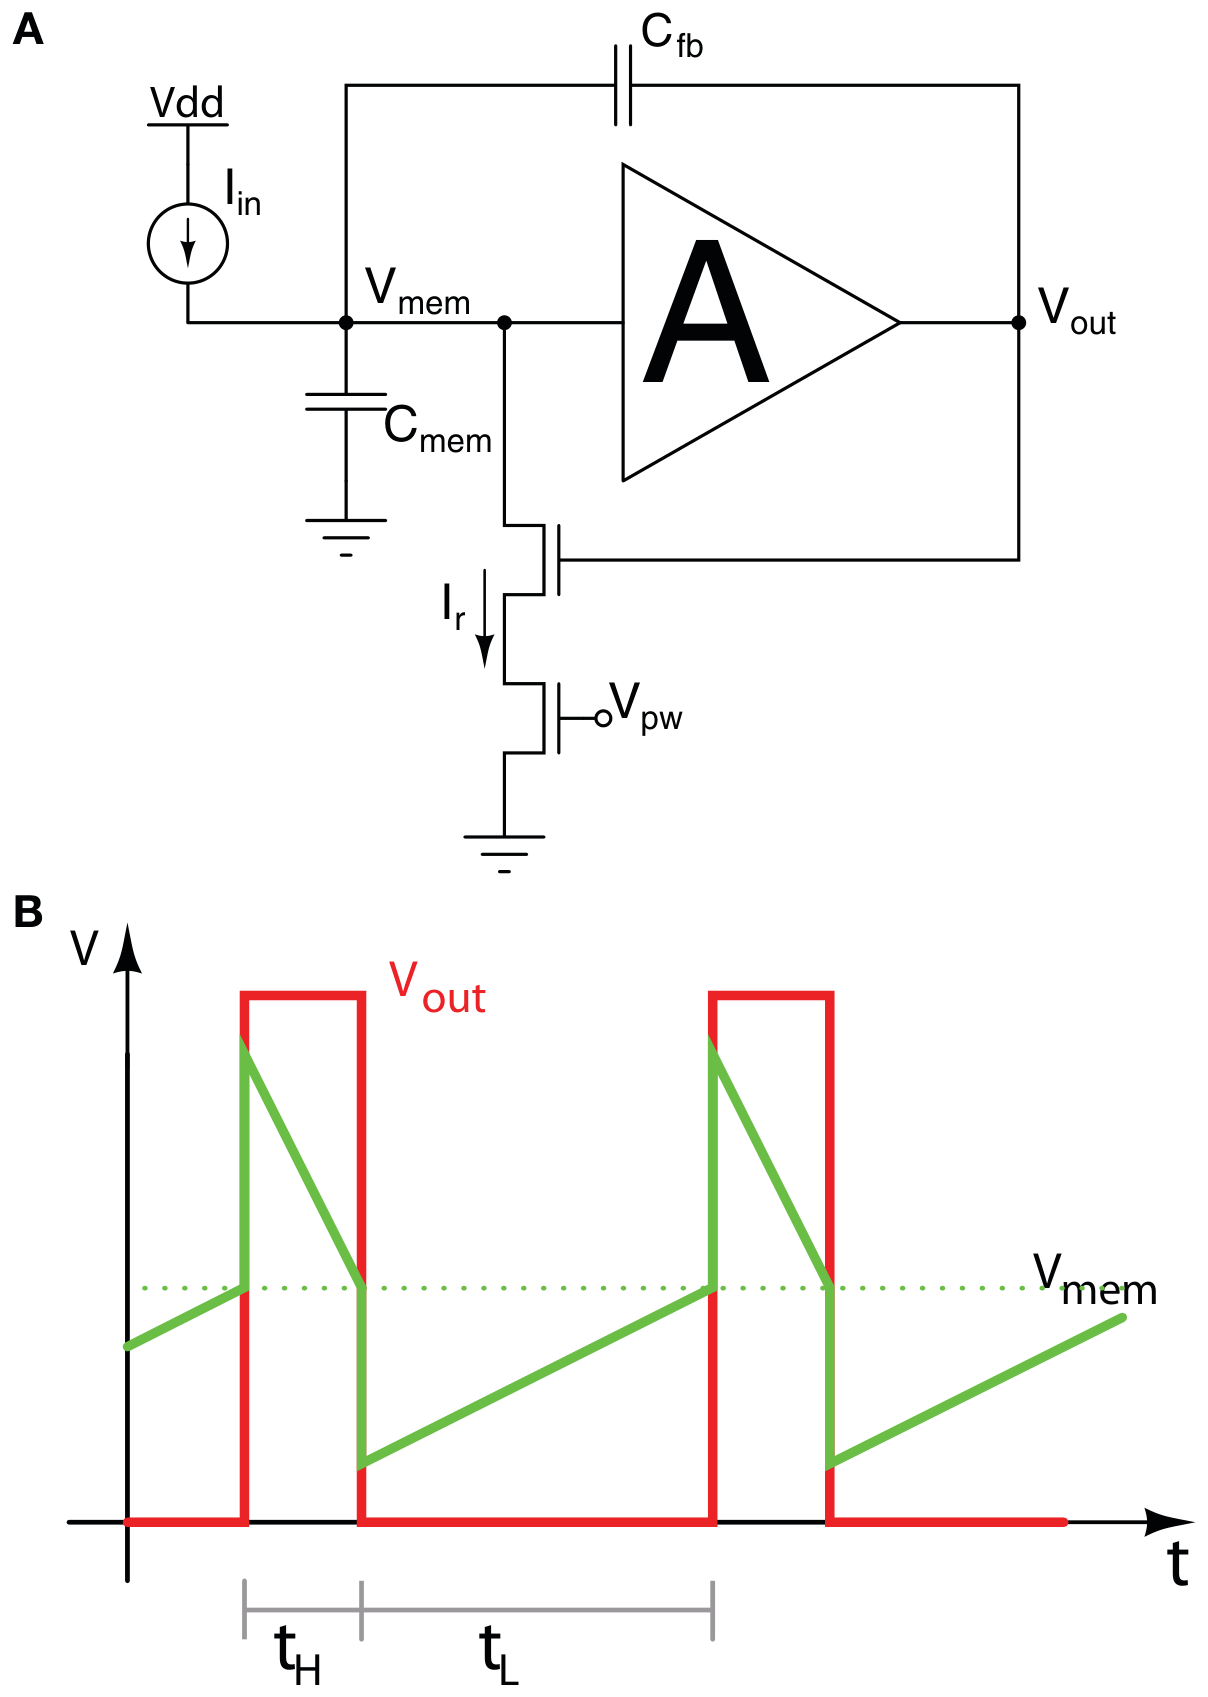
\includegraphics[width=\linewidth]{indiveri_axon_hillock.png}
    \caption{}
  \end{subfigure}
  \hfill
  \begin{subfigure}[b]{0.535\textwidth}
    \centering
    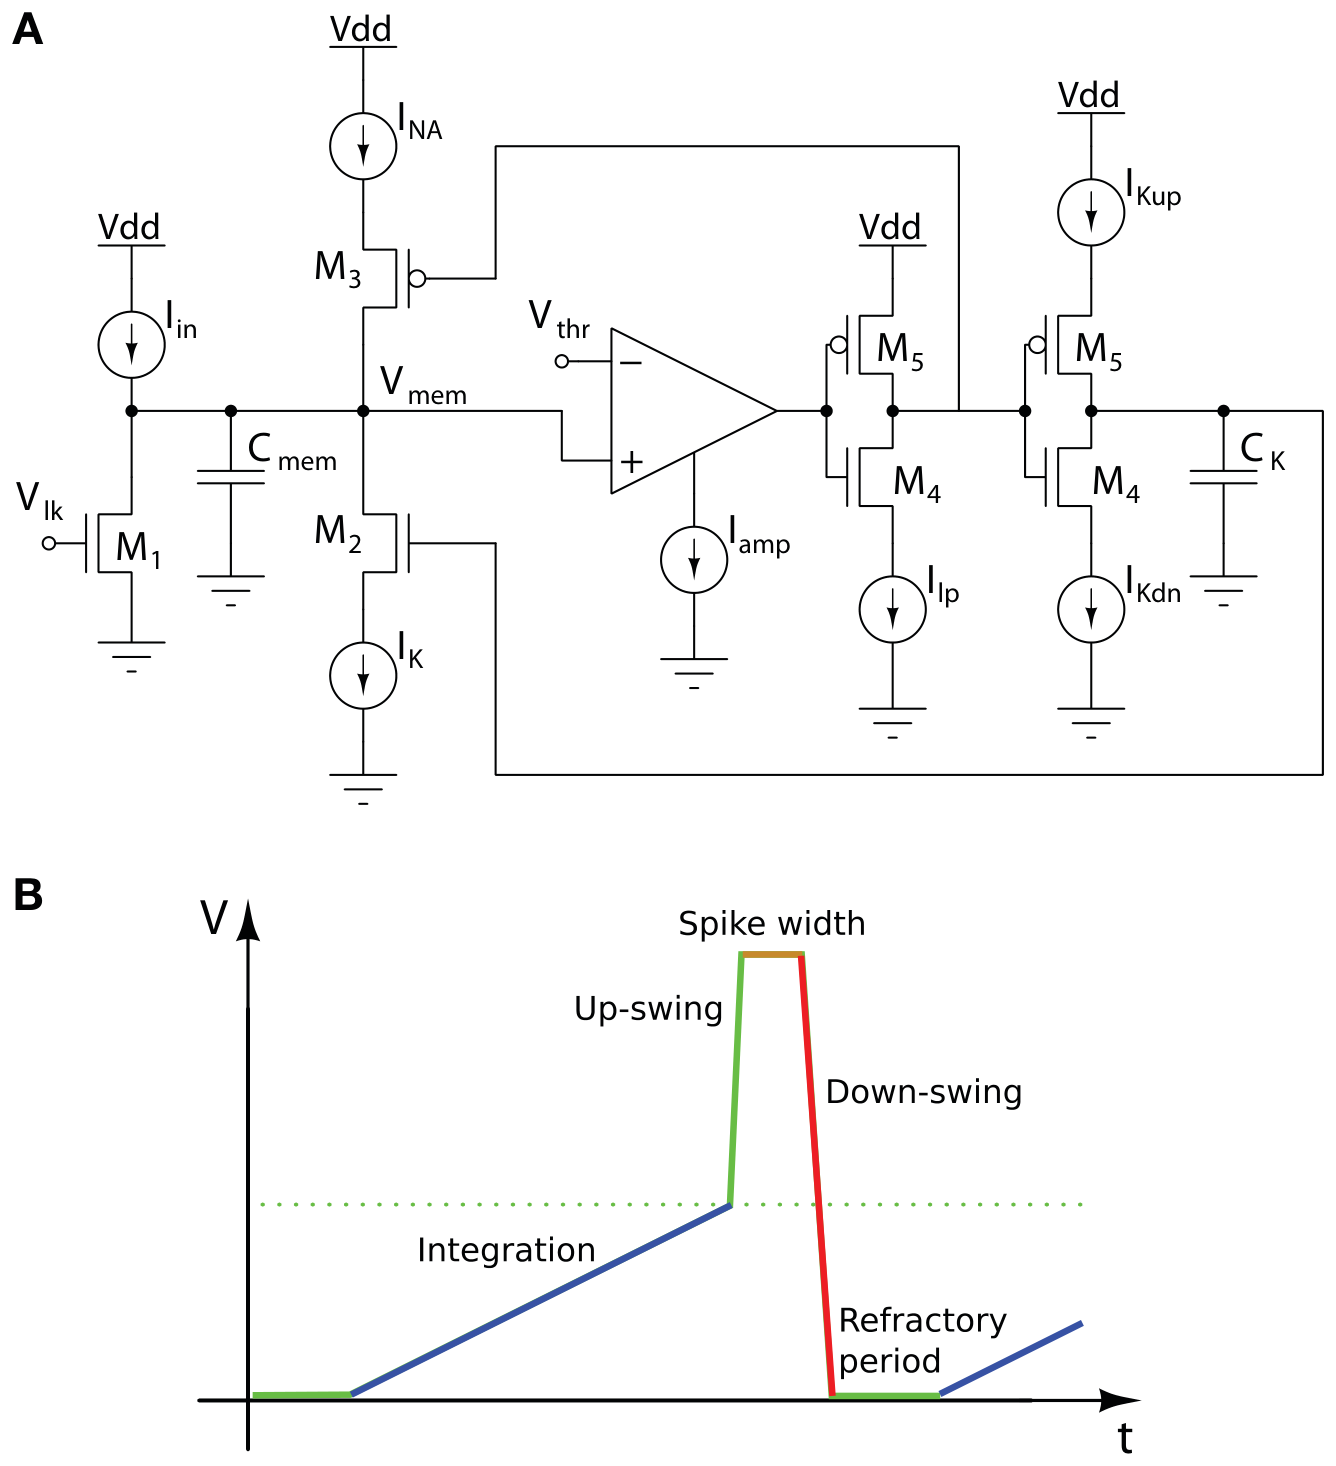
\includegraphics[width=\linewidth]{indiveri_vanschaik_ota.png}
    \caption{}
  \end{subfigure}
  \caption[]{(a) Circuito Axon-Hillock per la generazione dello spike, con schema elettrico (A) e andamento di $\Vmem$ e $V_{\mathrm{out}}$ (B); (b) Circuito di van Schaik per la generazione dello spike, con schema elettrico (A) e fasi dello spike su $\Vmem$ (B).}
  \label{fig:spike_gen}
\end{figure}

Per regolare la soglia di sparo e il periodo refrattario, van Schaik ha proposto il circuito mostrato in figura~\ref{fig:spike_gen}b~\cite{indiveri2011}. Qui il condensatore $\Cmem$ lavora assieme al transistor $M_1$ (controllato da $V_{\mathrm{lk}}$), che introduce una corrente di perdita verso massa. Se la corrente d'ingresso $\Iin$ supera questa perdita, $\Vmem$ sale e viene confrontata con una tensione di soglia  $\Vthr$ tramite un amplificatore a transconduttanza. Appena $\Vmem$ supera $\Vthr$, l'amplificatore commuta e pilota due inverter limitati in corrente (chiamati starved inverter, cioè inverter con un transistor in serie che ne fissa la corrente massima), usati per imitare l'apertura e la chiusura dei canali del sodio e del potassio~\cite{indiveri2011}. Il primo inverter accende $M_3$ lasciando scorrere la corrente $I_{\mathrm{Na}}$, che tira verso l'alto $\Vmem$. Invece il secondo inverter carica il condensatore $C_K$ con una velocità fissata dalla corrente $I_{\mathrm{Kup}}$. Quando la tensione su $C_K$ diventa abbastanza alta da accendere $M_2$, la corrente $I_K$ scarica $\Cmem$ riportando giù $\Vmem$. Quindi la corrente $I_{\mathrm{Kup}}$ regola il ritardo con cui interviene $M_2$ e fissa di conseguenza la durata dello spike. Quando $\Vmem$ scende sotto $\Vthr$, la corrente $I_{\mathrm{Na}}$ si spegne e il secondo inverter inizia a scaricare $C_K$ attraverso la corrente $I_{\mathrm{Kdn}}$. Se $I_{\mathrm{Kdn}}$ è piccola, $C_K$ si scarica lentamente mantenendo acceso $M_2$, quindi finché $I_K$ continua a scaricare la membrana, nessuna corrente d'ingresso più piccola di $I_K$ riesce a far ripartire il neurone: abbiamo ottenuto un periodo refrattario regolabile~\cite{indiveri2011}.

Però anche usando inverter limitati in corrente, quando $\Vmem$ si avvicina lentamente alla soglia resta comunque una corrente di cortocircuito tra $\Vdd$ e massa. Per ridurre questo consumo, Indiveri et al.\ (2011)~\cite{indiveri2011} propongono una soluzione, che è stata adottata nel neurone Octopus Retina. Sostanzialmente al posto della retroazione capacitiva si usa una retroazione positiva in corrente, che riutilizza la corrente di cortocircuito stessa del generatore di spike per iniettare carica aggiuntiva all'ingresso e accelerare di circa $100$ volte il superamento della soglia. La potenza di generazione dello spike è ridotta di circa $25$ volte e scende a \SI{4}{\pico\joule\per\spike} in CMOS \SI{0{,}6}{\micro\meter}~\cite{indiveri2011}.

\subsubsection{Adattamento della frequenza, neurone DPI e altri stili realizzativi}
\label{subsec:famiglie_neuroni}

I circuiti appena visti sono già dei neuroni completi molto semplici, ma non includono ancora un meccanismo per rallentare la frequenza di sparo e generare bursting. Per ottenere anche questi comportamenti, bisogna aggiungere una seconda variabile di adattamento~\cite{indiveri2011}.

Questo si può fare utilizzando i blocchi log-domain visti in precedenza. L'esempio principale di circuito CMOS completo, usato poi nei processori ROLLS, DYNAPs e DYNAP-SE2, è il neurone DPI~\cite{indiveri2011, qiao2015, moradi2018, bartels2025}. Per questo circuito valgono le seguenti equazioni~\cite{indiveri2011}:
\begin{equation}
  \tau \frac{\mathrm{d}\Imem}{\mathrm{d}t} = -\Imem\!\left(1 + \frac{I_g}{I_\tau}\right) + I_{\mathrm{mem}\infty} + f(\Imem),
  \qquad
  \tau_g \frac{\mathrm{d}I_g}{\mathrm{d}t} = -I_g + I_{g\max}\,r(t),
  \label{eq:dpi_adex}
\end{equation}
dove $\tau = \Cmem\UT/(\kappa I_\tau)$ è la costante di tempo di membrana, $I_{\mathrm{mem}\infty}$ dipende dalla corrente d'ingresso $\Iin$, $f(\Imem)$ è un termine esponenziale e $r(t)$ vale $1$ durante lo spike e $0$ altrimenti~\cite{indiveri2011}.

Se la priorità è invece ridurre il mismatch, in Indiveri et al.\ (2011)~\cite{indiveri2011} vengono mostrate alcune soluzioni alternative alla sottosoglia. Lavorando in forte inversione ma senza usare condensatori esterni, si passa a circuiti con costanti di tempo molto più veloci di quelle biologiche ($10^3\text{--}10^5$ volte, come nel neurone quadratico di Izhikevich di Wijekoon e Dudek in CMOS \SI{0{,}35}{\micro\meter}, circa $10^4$ volte più veloce)~\cite{indiveri2011}. Se invece si vuole restare nell'ordine dei tempi biologici, il neurone di Mihalas--Niebur a capacità commutate usa interruttori comandati da più fasi di clock~\cite{indiveri2011}. Per compensare il mismatch si possono anche usare i blocchi Digi-MOS già visti, mentre per eliminarlo del tutto si può ricorrere a neuroni LIF interamente digitali, basati su sommatori e accumulatori~\cite{indiveri2011}.

\subsection{Analisi approfondita dei processori CMOS della bibliografia}
\label{subsec:processori_cmos}

\subsubsection{ROLLS (Qiao et al., 2015): processore mixed-signal con apprendimento on-line}
\label{subsec:rolls_cmos}

Il processore ROLLS (Reconfigurable On-Line Learning Spiking neuromorphic processor) mostrato nel paper di Qiao et al.~\cite{qiao2015}, è un chip mixed-signal progettato per realizzare reti neurali spiking riconfigurabili con apprendimento direttamente sul chip e in tempo reale. È fabbricato in CMOS \SI{180}{\nano\meter}, occupa un'area di \SI{51{,}4}{\milli\meter\squared} con circa 12,2 milioni di transistor e consuma in media circa \SI{4}{\milli\watt}~\cite{qiao2015}.

È fatto da 256 neuroni analogici AdEx-I\&F e da 128k sinapsi analogiche, divise in due matrici $256\times 256$: 64k sinapsi con plasticità a lungo termine (LTP) per l'apprendimento sul chip e 64k sinapsi programmabili con plasticità a breve termine (STP)~\cite{qiao2015}. Un blocco di demultiplexing permette inoltre di assegnare più righe di sinapsi a uno stesso neurone, sacrificando i neuroni non utilizzati~\cite{qiao2015}.

% --- FIGURA 3.3: Schema CMOS del neurone AdEx-I&F di ROLLS (da Qiao et al., 2015, Fig. 3) ---
\begin{figure}[tb]
  \centering
  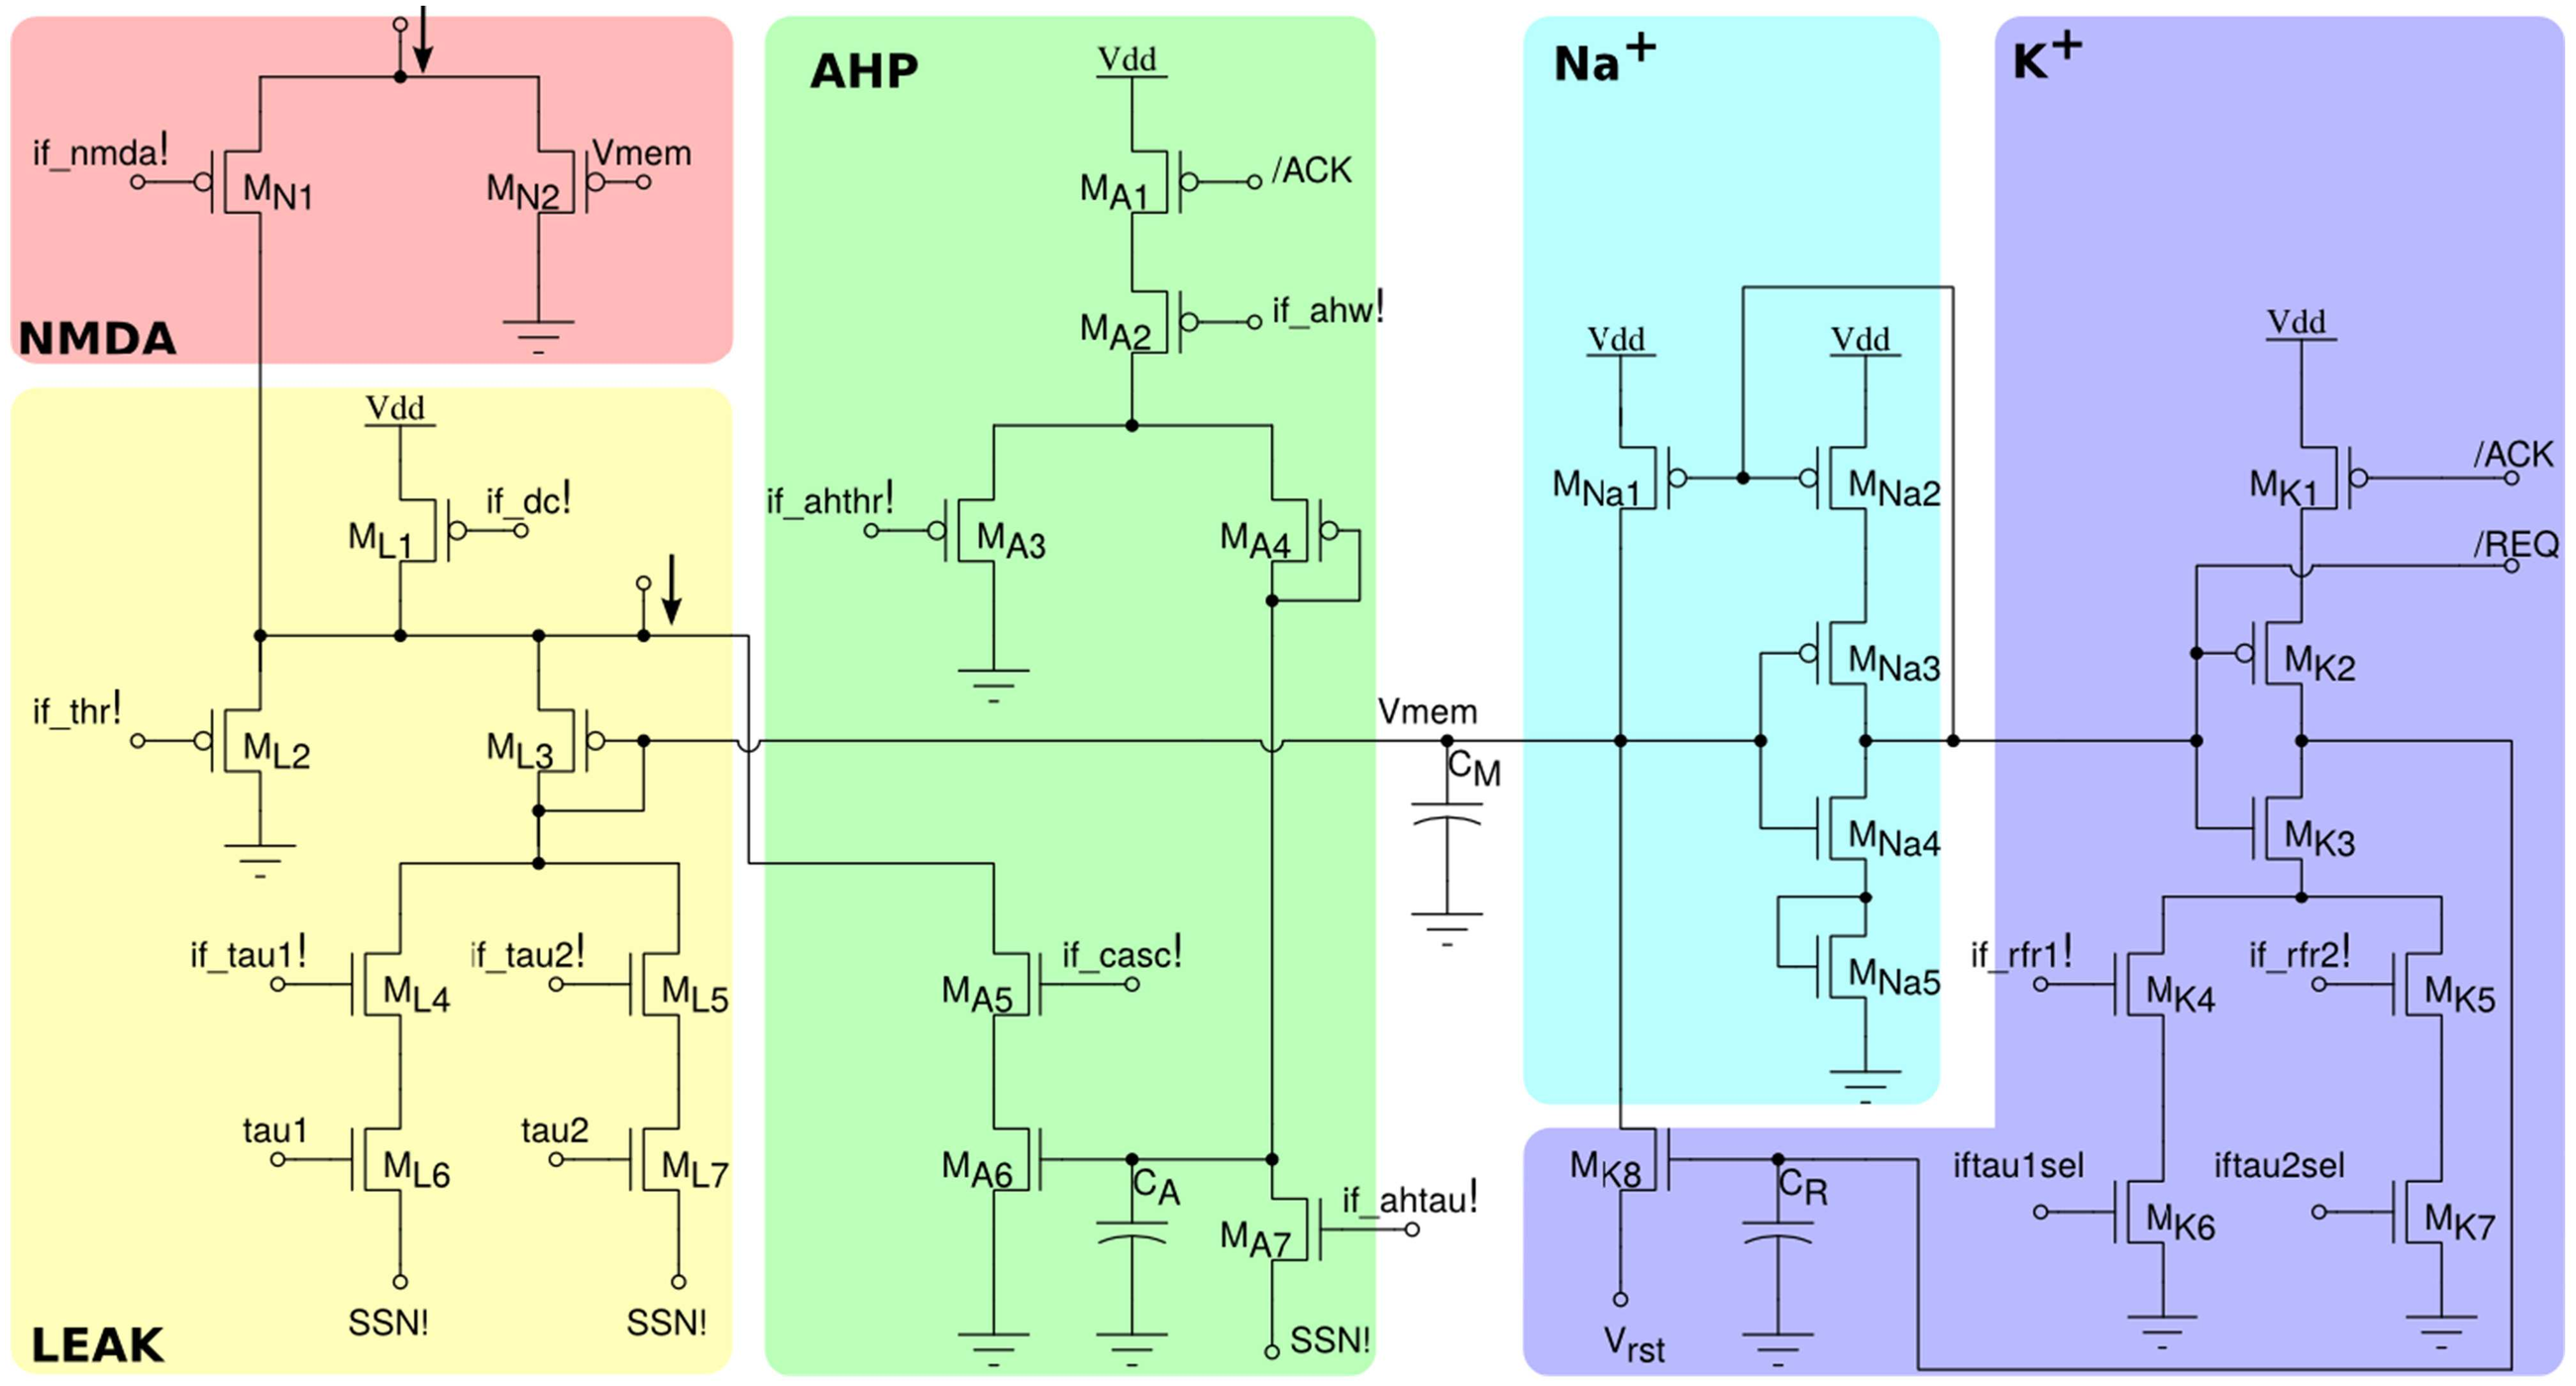
\includegraphics[width=\textwidth]{rolls_neuron_schematic.png}
  \caption[Schema CMOS del neurone AdEx-I\&F di ROLLS]{Schema a livello di transistor del neurone AdEx-I\&F del processore ROLLS~\cite{qiao2015}, suddiviso nei cinque blocchi funzionali (NMDA, LEAK, AHP, $\mathrm{Na}^+$ e $\mathrm{K}^+$).}
  \label{fig:rolls_neuron_schematic}
\end{figure}

In figura~\ref{fig:rolls_neuron_schematic} è riportato lo schema a livello di transistor del neurone di ROLLS~\cite{qiao2015}. Il circuito ha 13 bias regolabili (quelli indicati con il punto esclamativo nello schema) ed è organizzato in cinque blocchi. Il blocco NMDA ($M_{N1}, M_{N2}$) regola le correnti sinaptiche in funzione del potenziale di membrana $\Vmem$. Il blocco LEAK ($M_{L1}\text{--}M_{L7}$) è il circuito DPI d'ingresso che modella la perdita della membrana sulla capacità $C_M$. Sottolineo che usa la polarizzazione shifted-source (\texttt{SSN!}) vista in precedenza, per ottenere costanti di tempo biologiche. Il blocco AHP ($M_{A1}\text{--}M_{A7}$) integra gli spike emessi dal neurone sulla capacità $C_A$ (a ogni conferma \texttt{/ACK} ricevuta dal bus AER) e produce una corrente che frena il neurone, ottenendo adattamento della frequenza e bursting. Il blocco $\mathrm{Na}^+$ ($M_{\mathrm{Na1}}\text{--}M_{\mathrm{Na5}}$) applica la retroazione positiva in corrente al superamento della soglia per far salire rapidamente lo spike, imitando i canali del sodio. Infine il blocco $\mathrm{K}^+$ ($M_{K1}\text{--}M_{K8}$) segnala lo spike al bus AER tramite il segnale di richiesta \texttt{/REQ} (per trasmettere l'indirizzo del neurone), imposta il periodo refrattario tramite il condensatore $C_R$ e riporta $\Vmem$ al potenziale di reset regolabile $V_{\mathrm{rst}}$~\cite{qiao2015}. Inoltre, potendo selezionare digitalmente per ogni neurone tra due costanti di tempo di perdita nel blocco LEAK e due periodi refrattari nel blocco $\mathrm{K}^+$, si possono configurare fino a quattro popolazioni diverse di neuroni sullo stesso chip~\cite{qiao2015}. I comportamenti misurati sul silicio (reset regolabile, periodo refrattario, adattamento della frequenza e bursting) sono mostrati in figura~\ref{fig:rolls_silicio}c~\cite{qiao2015}.

Un aspetto importante del progetto di ROLLS è la riduzione del mismatch analogico. In sottosoglia le variazioni tra transistor possono rendere i neuroni molto diversi tra loro; per limitare questo effetto, gli autori hanno aumentato in modo mirato le dimensioni dei transistor più critici del soma, cioè quelli che fissano la costante di tempo di perdita ($M_{L4}$ e $M_{L5}$, con $W/L = \SI{2}{\micro\meter}/\SI{4}{\micro\meter}$) e la soglia di sparo ($M_{\mathrm{Na3}}$ da $\SI{4}{\micro\meter}/\SI{0{,}4}{\micro\meter}$ e $M_{\mathrm{Na4}}$ da $\SI{1}{\micro\meter}/\SI{4}{\micro\meter}$). Come si vede dalla curva frequenza-corrente in figura~\ref{fig:rolls_silicio}b, il mismatch medio su tutti i 256 neuroni scende così al 9,4\%, un valore molto contenuto per circuiti analogici in sottosoglia~\cite{qiao2015}.

\begin{figure}[tb]
  \centering
  \begin{subfigure}[b]{0.48\textwidth}
    \centering
    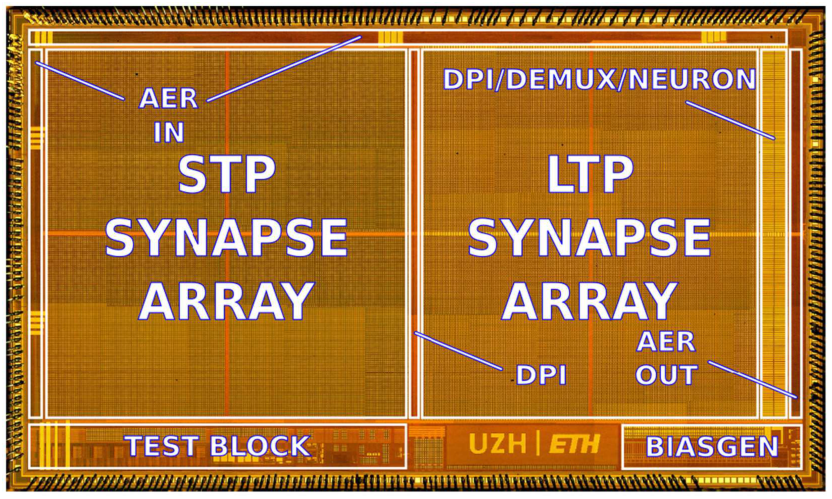
\includegraphics[width=\linewidth]{rolls_die.png}
    \caption{}
  \end{subfigure}
  \hfill
  \begin{subfigure}[b]{0.48\textwidth}
    \centering
    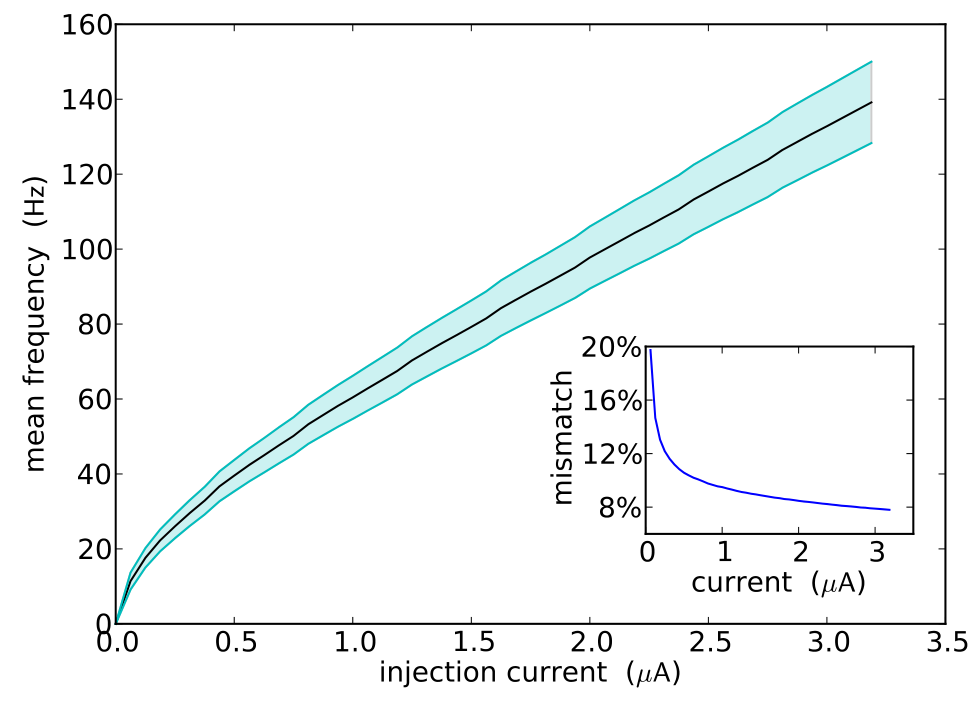
\includegraphics[width=\linewidth]{rolls_fi_mismatch.png}
    \caption{}
  \end{subfigure}
  \vspace{0.3cm}
  \begin{subfigure}[b]{0.92\textwidth}
    \centering
    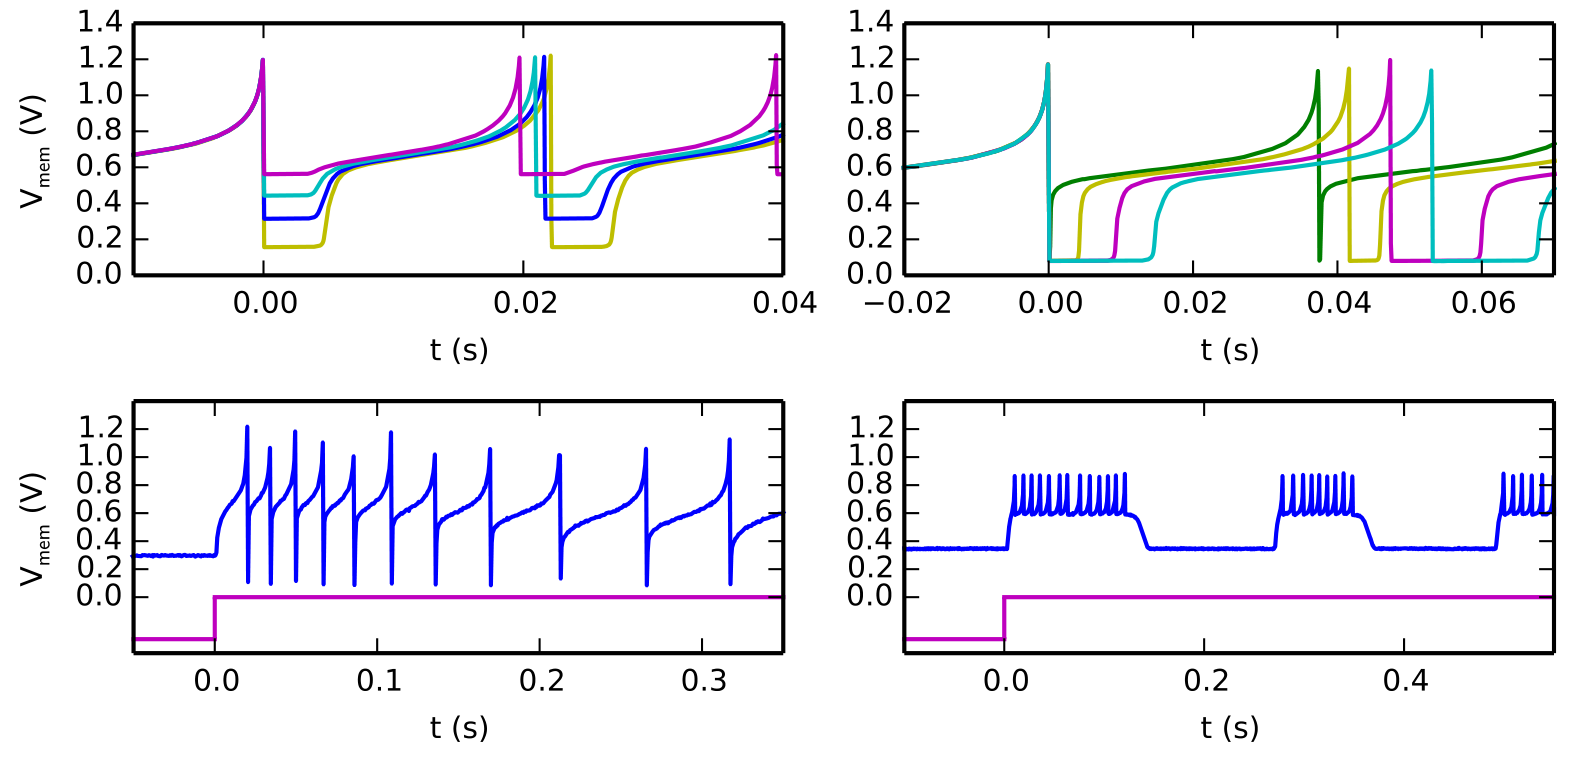
\includegraphics[width=\linewidth]{rolls_behaviors.png}
    \caption{}
  \end{subfigure}
  \caption[Caratterizzazione sperimentale del processore ROLLS]{Caratterizzazione sperimentale di ROLLS~\cite{qiao2015}: (a) microfotografia del die (\SI{51{,}4}{\milli\meter\squared} in CMOS \SI{180}{\nano\meter}); (b) curva frequenza-corrente media e deviazione standard dei 256 neuroni (mismatch medio 9,4\%); (c) andamenti misurati di $\Vmem$ per reset regolabile, periodo refrattario, adattamento della frequenza e bursting.}
  \label{fig:rolls_silicio}
\end{figure}

Per quanto riguarda le sinapsi, ROLLS adotta due soluzioni principali. La prima serve a risparmiare area: assumendo che le sinapsi di una stessa riga condividano le stesse costanti di tempo, le loro correnti d'uscita vengono sommate sfruttando la legge di Kirchhoff in un unico circuito DPI condiviso per riga (un DPI lento di tipo NMDA nella matrice LTP con costanti di tempo di centinaia di millisecondi, e due DPI più veloci di tipo AMPA e GABA nella matrice STP con costanti di tempo di decine di millisecondi)~\cite{qiao2015}. La seconda riguarda l'apprendimento e la conservazione dei pesi nel tempo. Nella matrice LTP i pesi analogici vengono aggiornati secondo la regola bistabile con stop-learning di Brader et al.\ (2007): all'arrivo di uno spike pre-sinaptico, la tensione interna $V_w$ che rappresenta il peso viene aumentata o diminuita in base al potenziale di membrana $\Vmem$ e all'attività recente del neurone post-sinaptico (modellata come una concentrazione di calcio misurata da un circuito DPI dedicato e confrontata con tre soglie per decidere se aggiornare o fermare l'apprendimento); in parallelo, un amplificatore a retroazione positiva spinge lentamente $V_w$ verso uno dei due stati stabili (alto o basso), evitando che il peso analogico vada alla deriva sul lungo periodo~\cite{qiao2015}. Nella matrice STP, invece, ogni sinapsi ha un peso digitale programmabile a 2 bit (quattro livelli), un bit per impostarla come eccitatoria o inibitoria e, in modalità eccitatoria, un circuito analogico di depressione a breve termine (STD) che riduce temporaneamente l'ampiezza della corrente durante raffiche di spike ravvicinati~\cite{qiao2015}.

Nonostante la condivisione dei circuiti DPI per riga, la ripartizione dell'area del chip (visibile anche in figura~\ref{fig:rolls_silicio}a) mette in evidenza un risultato molto significativo: i 256 neuroni ($55{,}69 \times \SI{16{,}48}{\micro\meter\squared}$ ciascuno, pari a \SI{0{,}235}{\milli\meter\squared} in totale) occupano solo lo 0,47\% dell'intera superficie del die, mentre le 128k sinapsi LTP (31,41\%) e STP (33,32\%) assorbono insieme il 64,73\% dell'area (\SI{33{,}28}{\milli\meter\squared}), con il resto occupato da generatore di bias, interfacce AER, logica di supporto e pad~\cite{qiao2015}.

\subsubsection{NET-TEN (Ronchini et al., 2023): rete analogica ultra-low-power a 250 mV}
\label{subsec:netten_cmos}

A differenza di un processore general-purpose riconfigurabile come ROLLS, \textbf{NET-TEN}~\cite{ronchini2023} dimostra cosa accade quando l'intera architettura CMOS viene progettata su misura per un'applicazione impiantabile, eliminando routing digitale, memorie SRAM/CAM e BiasGen integrati. Fabbricato anch'esso in CMOS \SI{180}{\nano\meter} ma alimentato a soli \textbf{$\Vdd = \SI{250}{\milli\volt}$}, il chip occupa \SI{1{,}08}{\milli\meter\squared} e integra 30 neuroni Izhikevich sottosoglia organizzati in 3 strati \emph{feed-forward} sparsi (10--10--10, con fan-in e fan-out pari a 2 tra primo e secondo strato e connessioni 1-a-1 tra strato nascosto e uscita) più 30 sinapsi EPSC+STDP (Figura~\ref{fig:netten_circuits})~\cite{ronchini2023}.

% --- FIGURA 3.5: Topologia, Neurone Izhikevich, EPSC e STDP di NET-TEN (da Ronchini et al., 2023, Fig. 3) ---
\begin{figure}[tb]
  \centering
  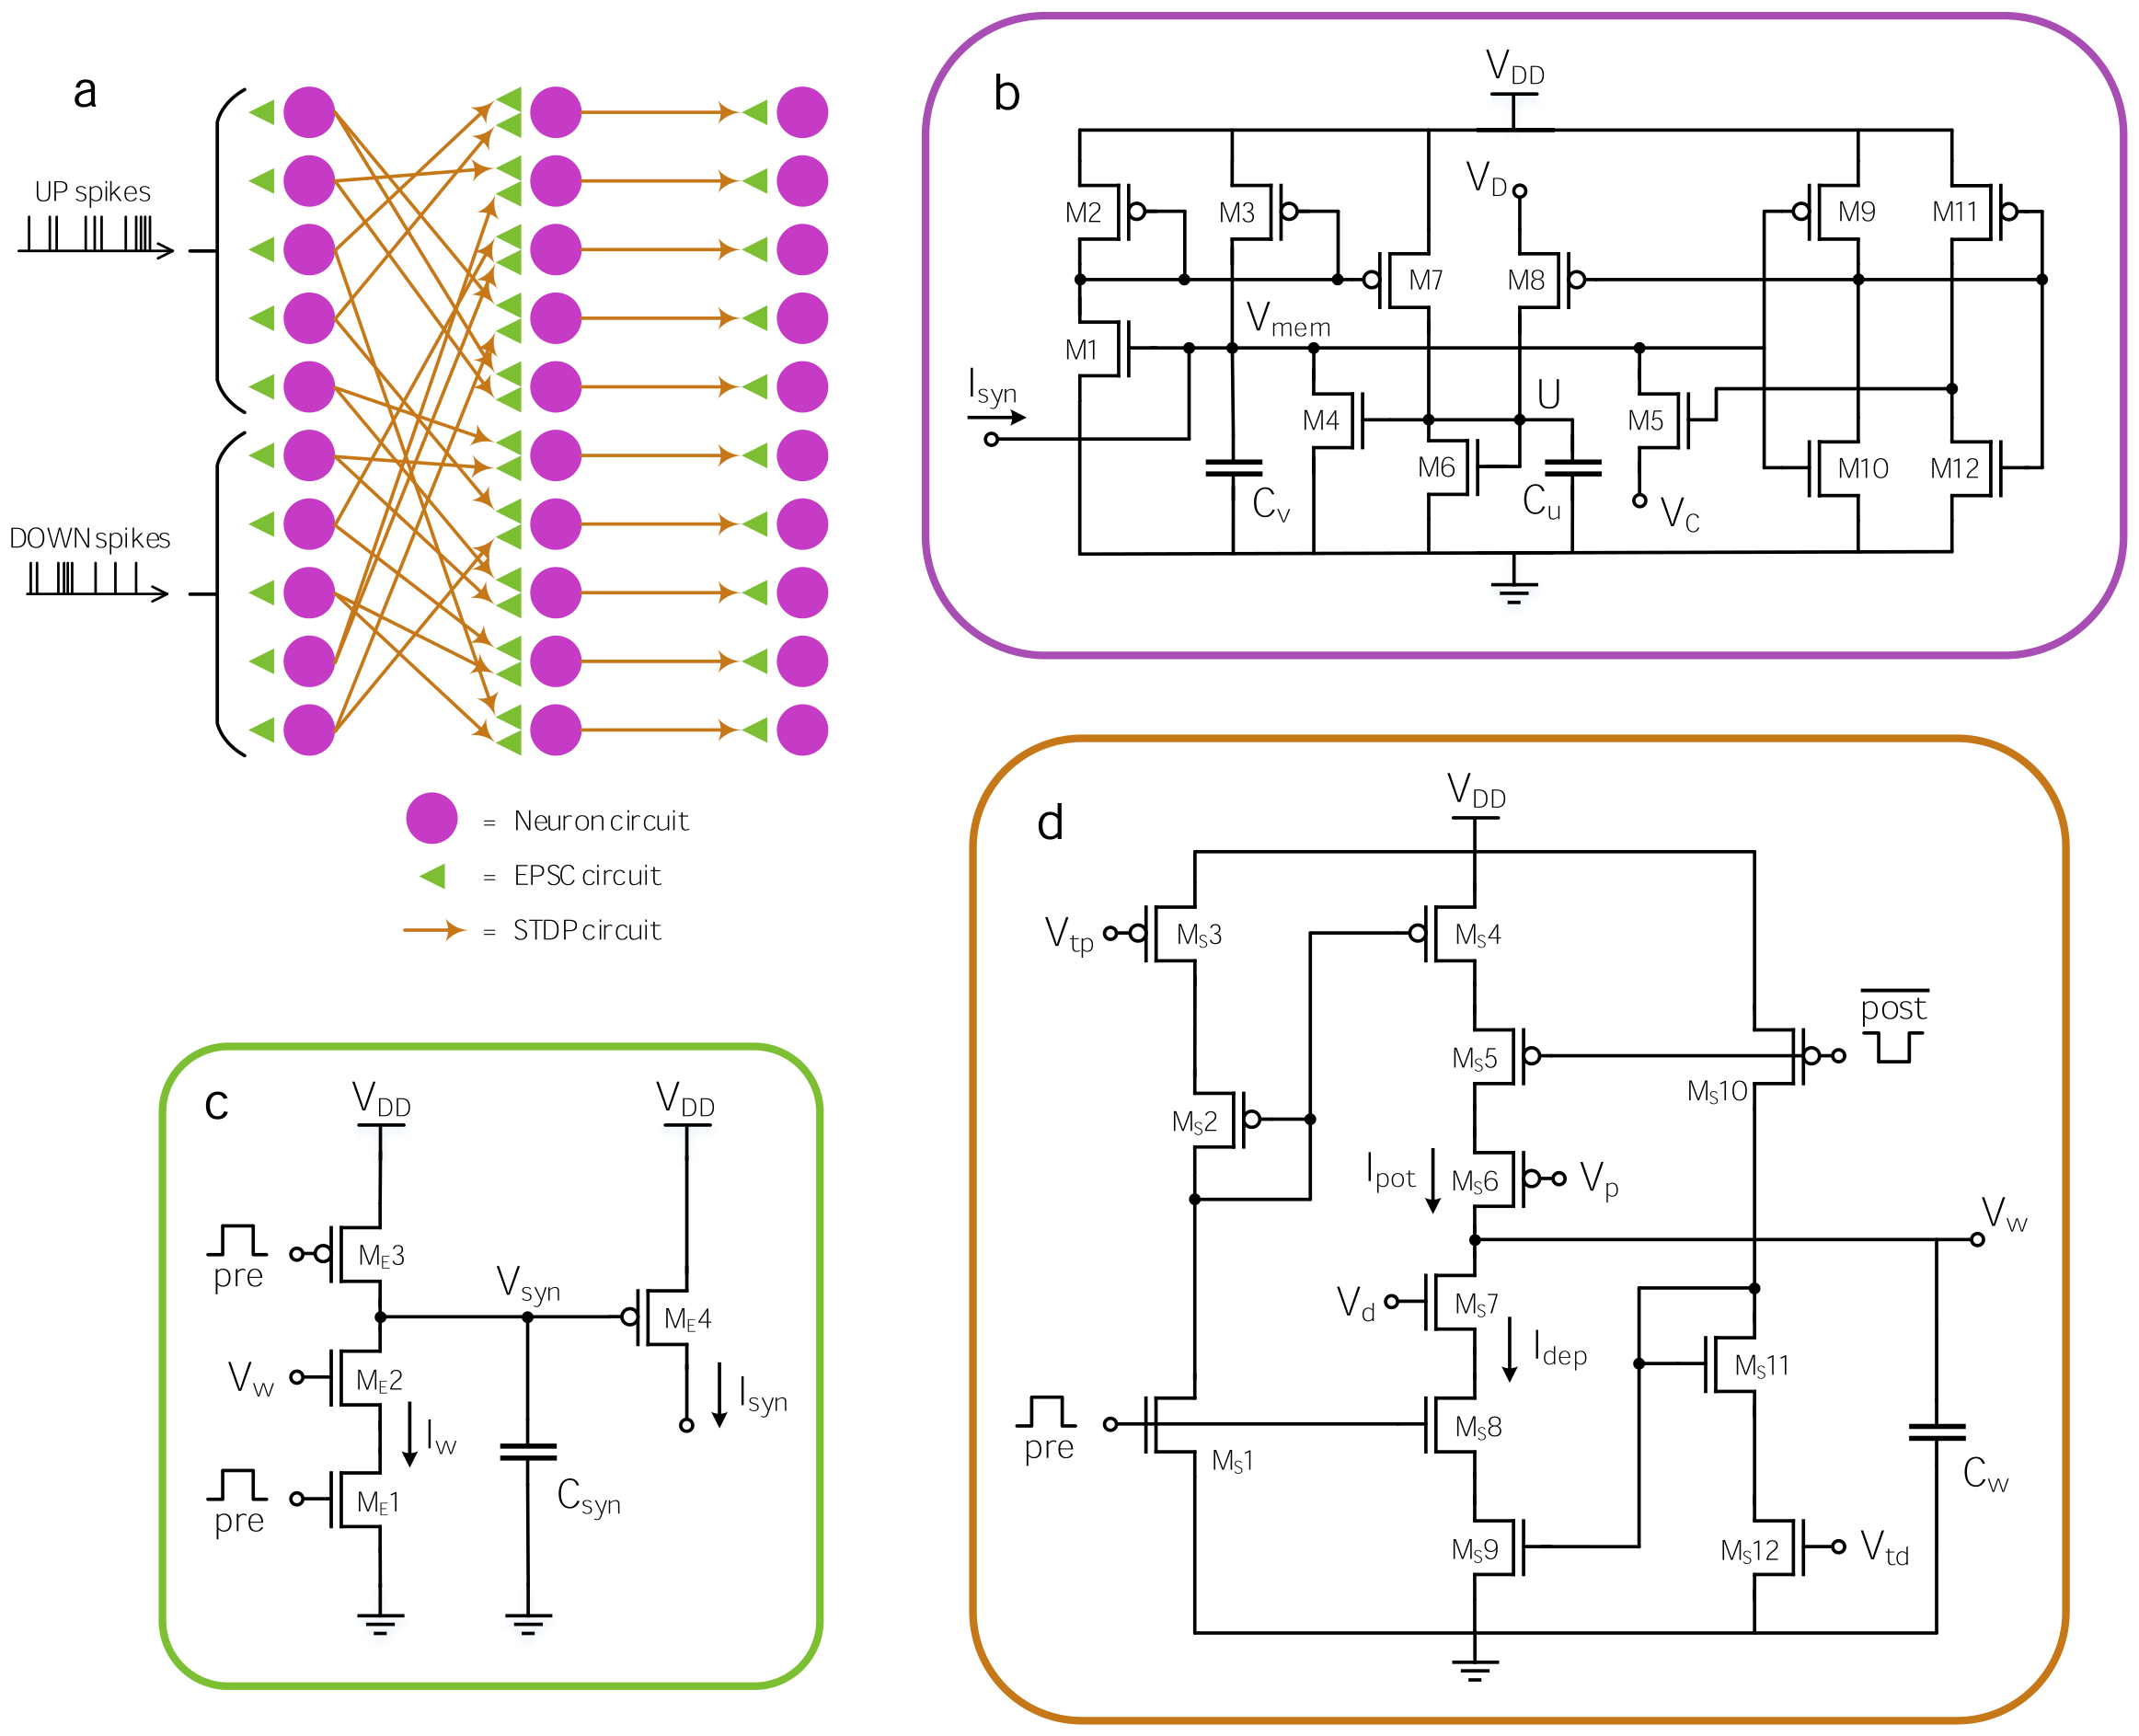
\includegraphics[width=0.90\textwidth]{netten_circuits.png}
  \caption[Topologia e schemi CMOS sottosoglia di NET-TEN]{Architettura e schemi CMOS sottosoglia di NET-TEN~\cite{ronchini2023} ($\Vdd = \SI{250}{\milli\volt}$): (a) topologia \emph{feed-forward} sparsa a 3 strati da 10 neuroni ciascuno; (b) neurone Izhikevich \emph{voltage-mode} ($M_1\text{--}M_{12}$, $C_v = \SI{76{,}86}{\femto\farad}$, $C_u = \SI{614{,}88}{\femto\farad}$, area \SI{1476{,}84}{\micro\meter\squared}); (c) generatore EPSC ($M_{E1}\text{--}M_{E4}$, picco \SI{486{,}39}{\pico\ampere}, $\tau = \SI{212{,}83}{\micro\second}$, area \SI{462{,}09}{\micro\meter\squared}); (d) circuito STDP sottosoglia ($M_{S1}\text{--}M_{S12}$, $C_w = \SI{206{,}30}{\femto\farad}$, area \SI{1054{,}75}{\micro\meter\squared}). Riprodotto da Ronchini et al.\ (2023)~\cite{ronchini2023}, licenza CC BY 4.0.}
  \label{fig:netten_circuits}
\end{figure}

Nel neurone di NET-TEN (Figura~\ref{fig:netten_circuits}b, area \SI{1476{,}84}{\micro\meter\squared}), le due variabili di stato del modello di Izhikevich ($\Vmem$ e $U$) risiedono sui condensatori integrati $C_v = \SI{76{,}86}{\femto\farad}$ e $C_u = \SI{614{,}88}{\femto\farad}$ (ottimizzati mediante analisi Monte Carlo per attenuare le variazioni di processo). Lo specchio $M_1\text{--}M_3$ applica un feedback positivo su $\Vmem$, bilanciato dalla corrente di leak $I_{M4}$ controllata da $U$; lo specchio $M_1, M_2, M_7$ accoppia $\Vmem$ a $U$, mentre $M_6$ fornisce il decadimento negativo su $C_u$. Due inverter in cascata ($M_9\text{--}M_{12}$) fungono da comparatore a soglia fissa generando sia l'impulso negativo di reset di $U$ (tramite $M_8$ e $V_D$) sia quello positivo di reset di $\Vmem$ (tramite $M_5$ e $V_C$). Il circuito EPSC ($M_{E1}\text{--}M_{E4}$, area \SI{462{,}09}{\micro\meter\squared}, Figura~\ref{fig:netten_circuits}c) precarica $C_{\mathrm{syn}}$ a $\Vdd$ tramite $M_{E3}$ e lo scarica all'arrivo dello spike \texttt{pre} con una corrente proporzionale al peso $V_w$, producendo su $M_{E4}$ (in sottosoglia) una corrente post-sinaptica esponenziale con picco di \SI{486{,}39}{\pico\ampere} e costante di tempo $\tau = \SI{212{,}83}{\micro\second}$ (a $V_w = \SI{200}{\milli\volt}$). Infine, il circuito STDP sottosoglia (derivato da Indiveri, area \SI{1054{,}75}{\micro\meter\squared}, Figura~\ref{fig:netten_circuits}d) memorizza il peso su $C_w = \SI{206{,}30}{\femto\farad}$, garantendo un'evoluzione adattativa su scale di decine di millisecondi~\cite{ronchini2023}.

NET-TEN mette in luce con grande chiarezza i due compromessi fisici del design interamente sottosoglia a \SI{250}{\milli\volt}:
\begin{itemize}
  \item \textbf{Variabilità (\emph{mismatch}) bifronte:} con bias globali identici, il \emph{mismatch} crea una naturale diversità funzionale fra neuroni (utile come espansione in caratteristiche casuali), ma oltre una certa soglia rende alcuni neuroni silenti o sempre attivi — motivo per cui solo 4 canali su 10 risultano utili e non sono identificabili a priori~\cite{ronchini2023}.
  \item \textbf{Ridotta capacità di pilotaggio (\emph{drivability}):} le correnti sub-nanoampere limitano il \emph{fan-out} senza ingrandire i transistori, imponendo la connettività sparsa (fan-out 2) e rendendo necessari buffer operazionali esterni (MAX44280, capacità d'ingresso \SI{0{,}4}{\pico\farad}) per osservare le uscite su PCB~\cite{ronchini2023}.
\end{itemize}

\subsubsection{DYNAPs (Moradi et al., 2018): scalabilità multi-core, memorie eterogenee e routing asincrono}
\label{subsec:dynaps_cmos}

Quando si passa da piccole reti dedicate (30 neuroni in NET-TEN) o da un singolo array (256 neuroni in ROLLS) a sistemi neuromorfici scalabili con migliaia o milioni di neuroni ed elevato \emph{fan-out} ($F \sim 10^3\text{--}10^4$), il vero collo di bottiglia non è più il circuito del singolo neurone, bensì la \textbf{memoria necessaria per memorizzare la connettività e l'energia per instradare gli spike}~\cite{moradi2018}.

In uno schema di routing convenzionale punto-punto per $N$ neuroni con fan-out $F$, ciascun neurone deve memorizzare $F \log_2(N)$ bit di indirizzi (es.\ \SI{160}{\kilo\bit\per\text{neurone}} per $N = 2^{20} \approx 10^6$ e $F \approx 10^4$). Per abbattere tale costo senza sacrificare la programmabilità né ricorrere a DRAM esterne, Moradi et al.\ (2018)~\cite{moradi2018} introducono nei processori \textbf{DYNAPs} (\emph{Dynamic Neuromorphic Asynchronous Processors}) uno \textbf{schema di routing a due stadi basato su tag condivisi}, ispirato alla connettività a cluster della corteccia cerebrale:
\begin{enumerate}
  \item i neuroni sono raggruppati in $N/C$ core (cluster) di dimensione $C$;
  \item nel \textbf{primo stadio} (routing sorgente punto-punto), il router locale \textbf{R1} legge una SRAM di sorgente e invia un \emph{tag} di $\log_2(K)$ bit a $F/M$ nodi intermedi (core di destinazione);
  \item nel \textbf{secondo stadio} (\emph{broadcast} locale), il tag viene diffuso a tutti i $C$ neuroni del core di destinazione, ciascuno dotato di una memoria associativa asincrona \textbf{CAM} (\emph{Content-Addressable Memory}) che accetta lo spike solo se il tag coincide con una delle sue sinapsi sottoscritte ($M$ neuroni sottoscritti per tag; Figura~\ref{fig:dynaps_routing}b).
\end{enumerate}

Minimizzando la somma di memoria sorgente $\mathrm{MEM}_S$ e memoria destinazione $\mathrm{MEM}_T$ rispetto al parametro di compromesso $M$ (con $\alpha = K/C = 1$), Moradi et al.\ dimostrano che la memoria per neurone si riduce a~\cite{moradi2018}:
\begin{equation}
  \mathrm{MEM} = \frac{F}{M}\log_2\!\left(\frac{KN}{C}\right) + \frac{KM}{C}\log_2(K)
  \;\xrightarrow[\alpha=1]{M = M^*}\;
  \mathrm{MEM}_{\min} = 2\sqrt{F \log_2(C)\log_2(N)}\;\;\text{bit/neurone}.
  \label{eq:dynaps_mem}
\end{equation}
Per una rete da un milione di neuroni ($N=2^{20}$, $F=2^{13}$, $C=256$), ciò abbatte la memoria da \textbf{160k bit/neurone a meno di 1,2k bit/neurone} (oltre $130\times$ di riduzione), assicurando inoltre uno scaling lineare anziché quadratico rispetto a IBM TrueNorth nell'implementazione di CNN~\cite{moradi2018}.

% --- FIGURA 3.6: Architettura di routing R1-R2-R3 e nodo eterogeneo DYNAPs (da Moradi et al., 2018, Fig. 2 e 9) ---
\begin{figure}[tbp]
  \centering
  \begin{subfigure}[b]{0.48\textwidth}
    \centering
    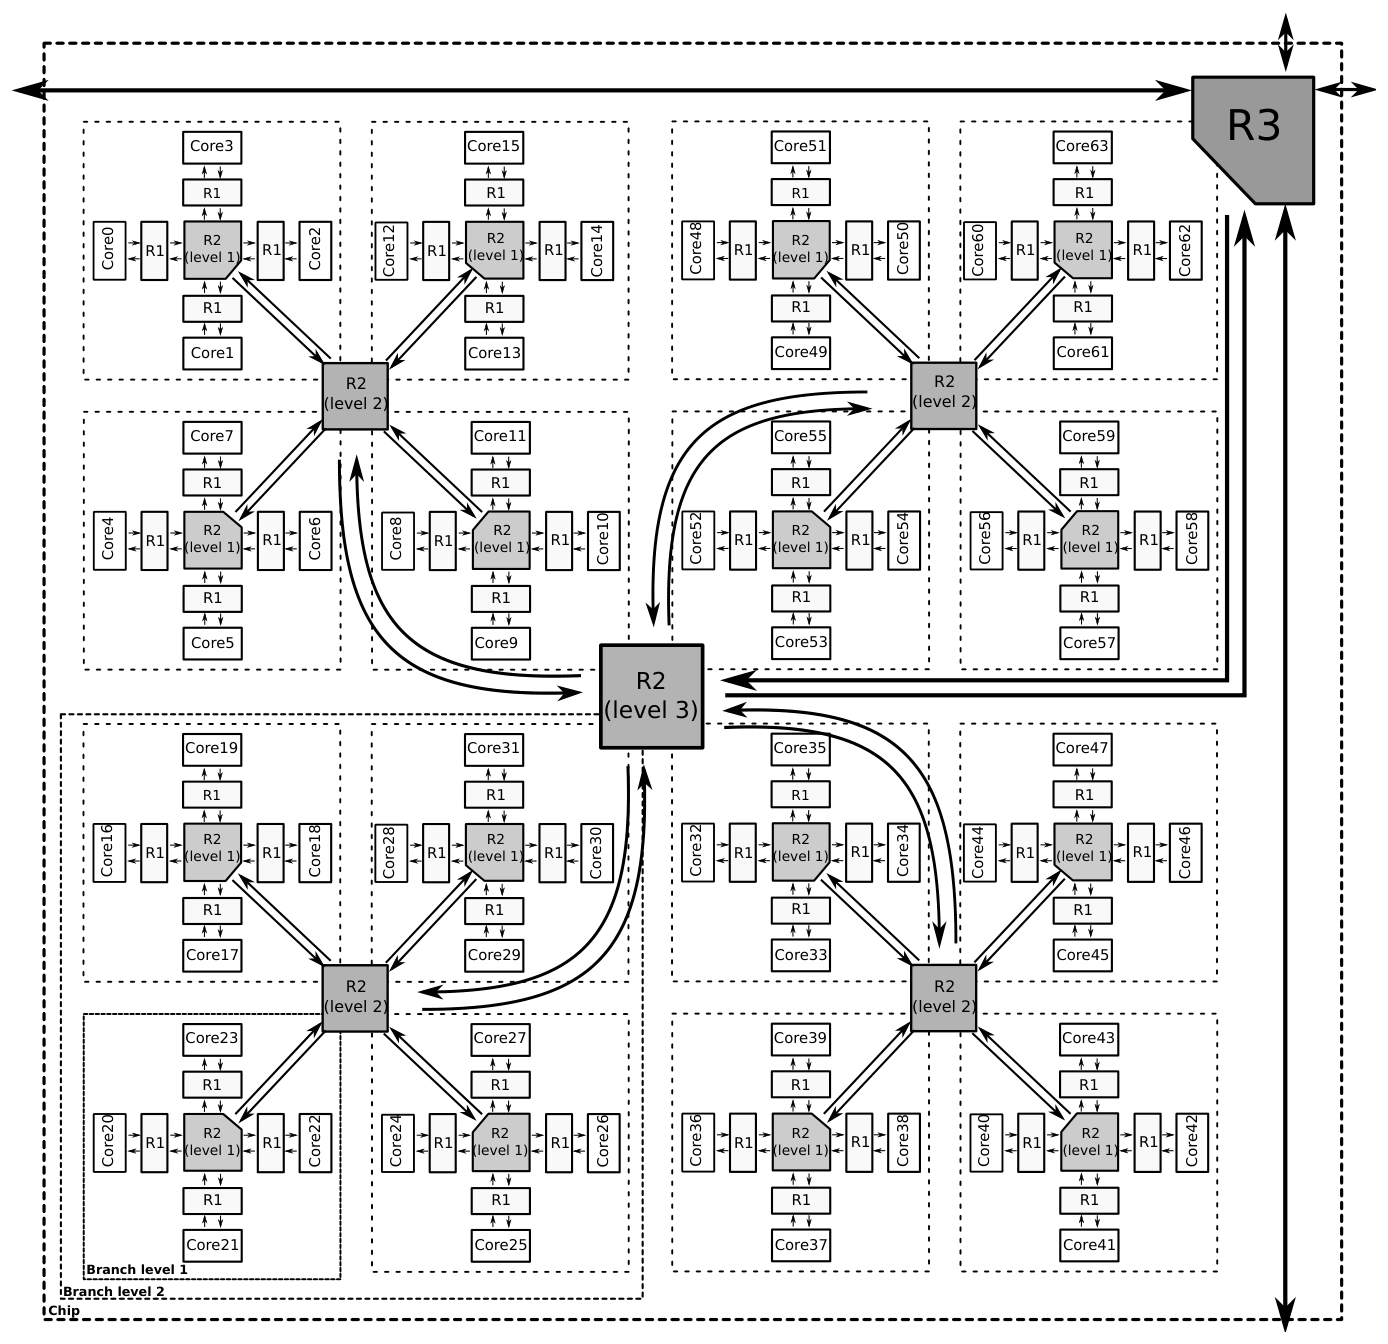
\includegraphics[width=\linewidth]{dynaps_routing_tree.png}
    \caption{Rete di routing gerarchica ad albero (R1, R2) e mesh 2D (R3).}
  \end{subfigure}

  \vspace{0.35cm}
  \begin{subfigure}[b]{0.76\textwidth}
    \centering
    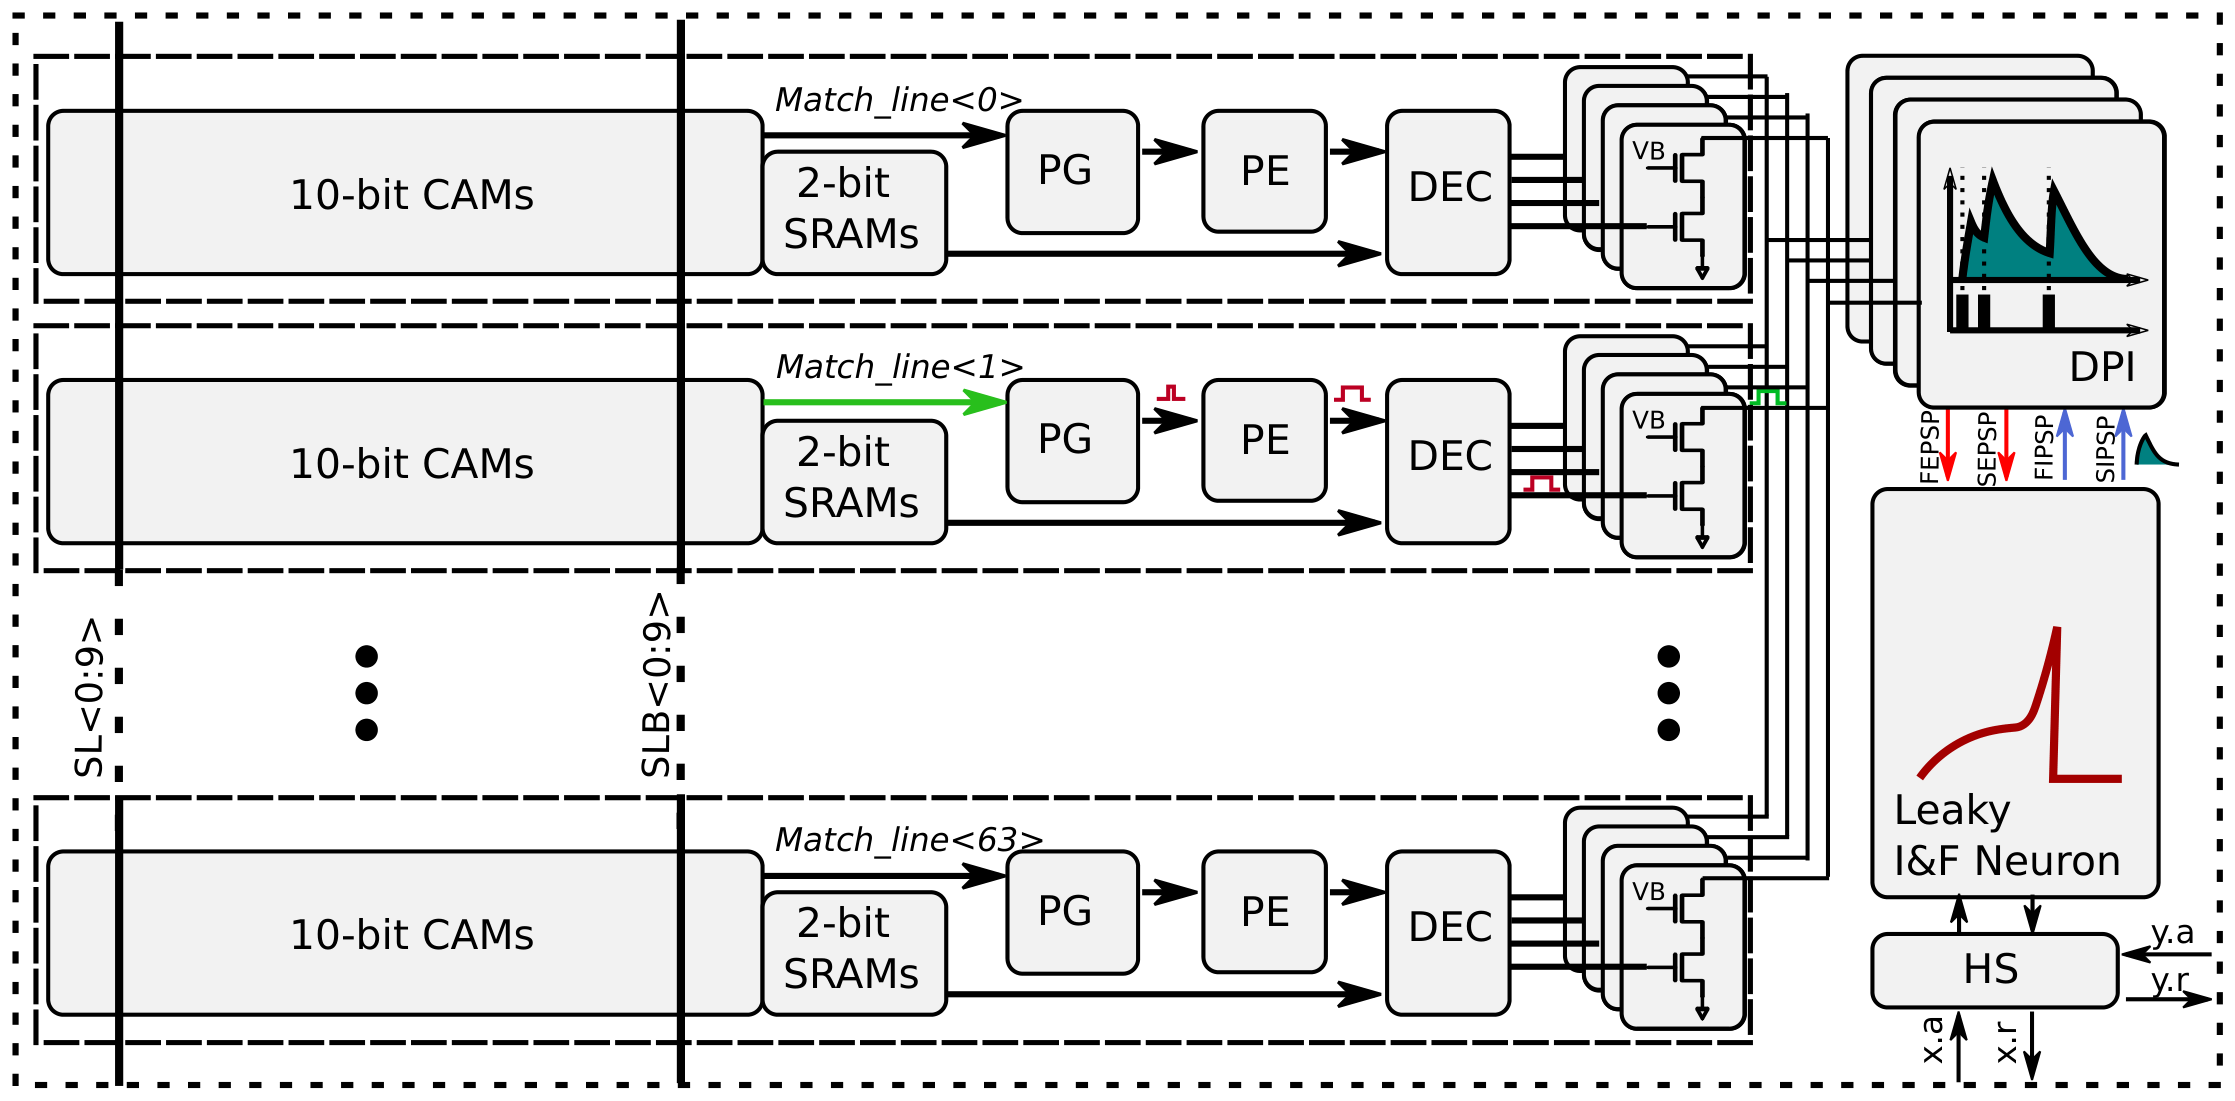
\includegraphics[width=\linewidth]{dynaps_node.png}
    \caption{Schema a blocchi di uno dei 256 nodi \emph{in-memory} di ciascun core.}
  \end{subfigure}
  \caption[Architettura di routing e nodo \emph{in-memory} di DYNAPs]{Architettura del processore multi-core DYNAPs~\cite{moradi2018}: (a) rete di routing asincrona QDI gerarchica (router locali R1 per core, R2 ad albero multi-livello intra-chip e R3 a mesh 2D XY tra chip); (b) struttura del singolo nodo di calcolo e memoria eterogenea distribuita (64 CAM da 10 bit, 64 SRAM da 2 bit, generatori/estensori/decodificatori d'impulsi PG/PE/DEC, 4 filtri DPI e 1 neurone analogico Leaky I\&F con blocco di handshaking HS). Riprodotto da Moradi et al.\ (2018)~\cite{moradi2018}.}
  \label{fig:dynaps_routing}
\end{figure}

Il chip prototipo DYNAPs è fabbricato in CMOS \SI{180}{\nano\meter} 1P6M (\SI{43{,}79}{\milli\meter\squared} totali, \SI{38{,}5}{\milli\meter\squared} di core) con tensione di alimentazione riducibile fino a \SI{1{,}3}{\volt} (nominale \SI{1{,}8}{\volt}), e integra \textbf{4 core da 256 neuroni} (1024 neuroni AdEx-I\&F DPI, 64k sinapsi con fan-in 64 e fan-out 4k, 64k celle CAM + 4k SRAM). I router R1, R2 e R3 (Figura~\ref{fig:dynaps_routing}a) sono sintetizzati con logica digitale asincrona \emph{Quasi Delay-Insensitive} (QDI) a codifica \emph{dual-rail} (latenza di attraversamento inter-chip di \SI{15{,}4}{\nano\second}, latenza interna di R3 di \SI{2{,}5}{\nano\second}, energia per \emph{hop} di \SI{17}{\pico\joule} a \SI{1{,}3}{\volt}, tempo di broadcast nella CAM di \SI{27}{\nano\second})~\cite{moradi2018}. Come visibile nella Figura~\ref{fig:dynaps_silicio}a (ingrandimento del nodo) e nella Tabella~I di Moradi et al.~\cite{moradi2018}, la memoria on-chip (31,7\%), gli estensori/decodificatori d'impulsi (25,2\%) e i router (9,7\%) occupano complessivamente il \textbf{66,6\%} dell'area core, mentre neuroni e sinapsi analogiche rappresentano solo il \textbf{22,8\%}. Ancora più illuminante è la Figura~\ref{fig:dynaps_silicio}b: al crescere della frequenza di firing fino a \SI{100}{\hertz}, la potenza della logica digitale di routing e CAM cresce molto più rapidamente di quella analogica, arrivando a rappresentare circa i due terzi della dissipazione totale a \SI{1{,}8}{\volt} ($\sim\SI{1{,}8}{\milli\watt}$ digitali su $\sim\SI{2{,}7}{\milli\watt}$ totali)~\cite{moradi2018}.

\begin{figure}[tb]
  \centering
  \begin{subfigure}[b]{0.52\textwidth}
    \centering
    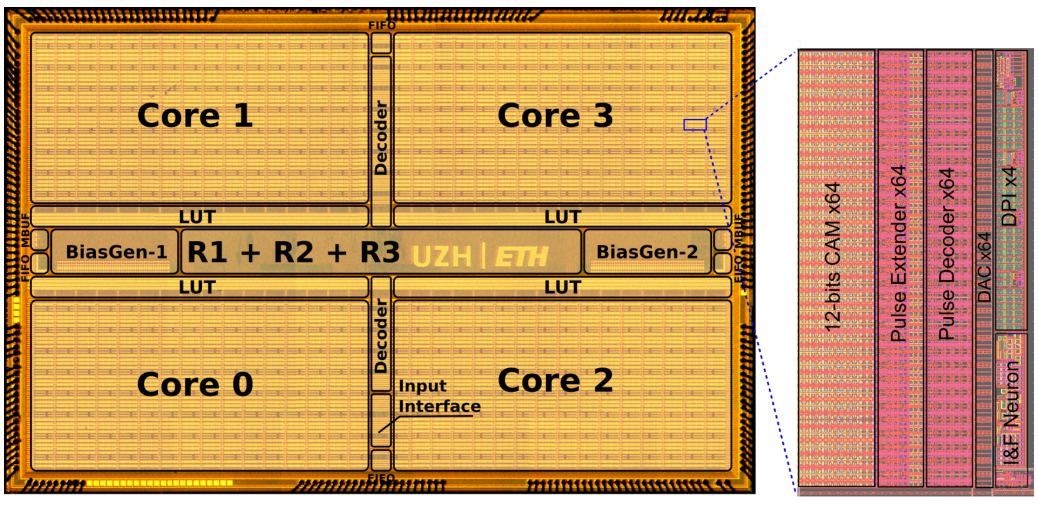
\includegraphics[width=\linewidth]{dynaps_die.png}
    \caption{Microfotografia del die DYNAPs (\SI{43{,}79}{\milli\meter\squared}) e zoom del nodo.}
  \end{subfigure}
  \hfill
  \begin{subfigure}[b]{0.45\textwidth}
    \centering
    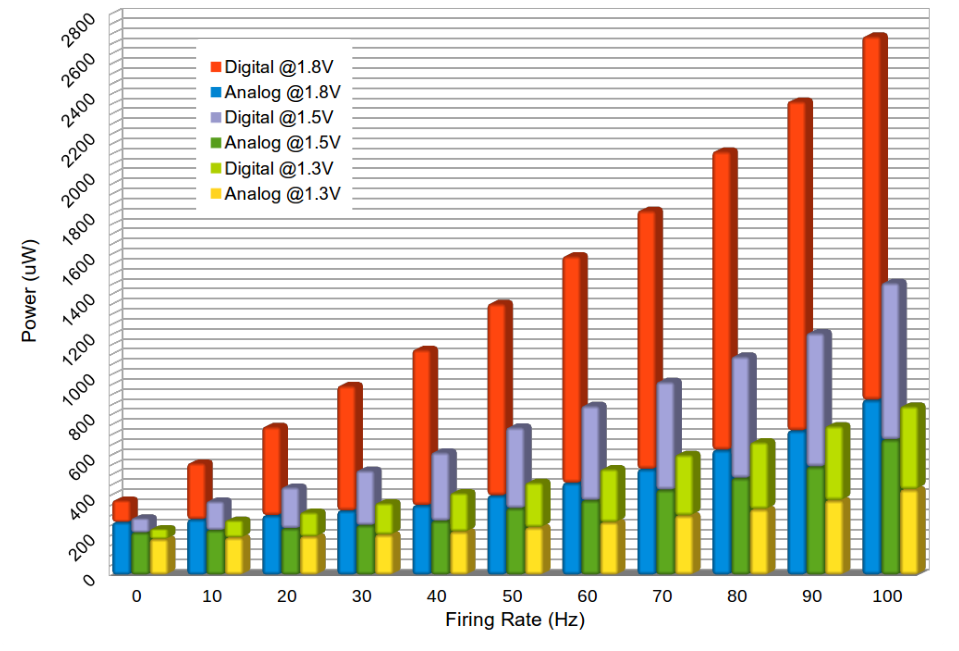
\includegraphics[width=\linewidth]{dynaps_power_freq.png}
    \caption{Potenza analogica e digitale misurata vs frequenza di firing.}
  \end{subfigure}
  \caption[Caratterizzazione hardware del processore DYNAPs]{Caratterizzazione hardware del processore multi-core DYNAPs~\cite{moradi2018}: (a) layout dei 4 core, router R1/R2/R3 e BiasGen, con dettaglio del singolo nodo che evidenzia l'ampia superficie occupata da CAM e Pulse Extender/Decoder rispetto al piccolo neurone I\&F e ai 4 DPI; (b) potenza totale impilata (analogica in basso, digitale in alto) al variare della frequenza di disparo di tutti i 1024 neuroni per $\Vdd = 1{,}3; 1{,}5; \SI{1{,}8}{\volt}$. Riprodotto da Moradi et al.\ (2018)~\cite{moradi2018}.}
  \label{fig:dynaps_silicio}
\end{figure}

L'evoluzione successiva \textbf{DYNAP-SE2} (utilizzata da Bartels et al.~\cite{bartels2025}) mantiene la medesima architettura \emph{mixed-signal} a 4 core in \SI{180}{\nano\meter} con neuroni AdEx-I\&F DPI e sinapsi a 4 tipi (AMPA, NMDA, GABA-A shunting, GABA-B), aggiungendo però l'AFE+ADM sullo stesso die e pesi a 4 bit; il suo \emph{mismatch} misurato sui parametri di bias sottosoglia ha un coefficiente di variazione (CV) del \textbf{20--30\%}, che gli autori compensano sfruttando la topologia ricorrente/NLNG anziché pesi precisi~\cite{bartels2025}. Per contrasto, il chip \textbf{Xylo} (Li et al.~\cite{li2024}) rappresenta il polo \textbf{interamente digitale} (CMOS \SI{28}{\nano\meter}, \SI{6{,}5}{\milli\meter\squared}, $\Vdd = \SI{1{,}8}{\volt}$ core / \SI{2{,}5}{\volt} I/O, clock fino a \SI{250}{\mega\hertz}, \SI{124}{\kilo\byte} SRAM): i 1000 neuroni LIF digitali con decadimento \emph{bit-shift} e pesi a 8 bit presentano \textbf{zero \emph{mismatch} analogico} e pieno supporto al training off-chip tramite BPTT, ma al prezzo di un consumo stabile di \SI{287{,}9}{\micro\watt} nel core (più \SI{87{,}4}{\micro\watt} I/O) e di una piccola perdita di accuratezza dovuta alla quantizzazione ($\sim 3{,}4\text{--}4{,}3$ punti percentuali)~\cite{li2024}.

\subsection{Tabelle comparative e risposta alla seconda domanda centrale}
\label{subsec:tabelle_cmos}

Le Tabelle~\ref{tab:confronto_neuroni} e~\ref{tab:confronto_sistemi} (riportate in formato orizzontale nelle pagine seguenti per la massima leggibilità) raccolgono sistematicamente tutti i parametri richiesti dalla consegna (tensione di alimentazione, consumo statico, potenza media, energia per spike, area, frequenza di firing e variabilità) rispettivamente a livello di singolo neurone CMOS e a livello di processore/sistema integrato. I campi non riportati esplicitamente dagli articoli originali sono indicati con ``\ND''.

\begin{sintesiBox}{Risposta alla Domanda Centrale 2: Come si realizza un neurone spiking in CMOS e quali compromessi emergono?}
Un neurone spiking CMOS integra quattro funzioni fisiche: accumulo di carica con perdita su una capacità di membrana ($\Cmem$), innesco rapido al superamento della soglia (tramite amplificatore/comparatore o feedback positivo in corrente), ripristino con periodo refrattario ($C_R$ / \emph{starved inverters}) ed eventualmente una seconda variabile lenta di adattamento (DPI di AHP o condensatore $C_u$). Le architetture proposte evidenziano un compromesso netto tra quattro assi:
\begin{itemize}
  \item \textbf{Analogico sottosoglia puro (DPI, Izhikevich a \SI{250}{\milli\volt}):} minimizza tensione, potenza (pW--nW) e area con costanti di tempo biologiche naturali \emph{real-time}, ma soffre di \textbf{elevata variabilità (\emph{mismatch} 9--30\%)} e ridotta capacità di pilotaggio, richiedendo sovradimensionamento selettivo (ROLLS), reti tolleranti alla topologia (DYNAP-SE2) o apprendimento/calibrazione.
  \item \textbf{Mixed-signal (neuroni analogici + routing/memorie digitali asincrone):} consente reti scalabili, programmabili e multi-core (ROLLS, DYNAPs, DYNAP-SE2), ma sposta gran parte di area ed energia dalle celle neuronali alle sinapsi, alle CAM e al routing AER.
  \item \textbf{Soprasoglia accelerato e Switched-Capacitor:} abbatte drasticamente il \emph{mismatch} e offre alta ripetibilità (10 regimi in Mihalas--Niebur S-C; $<10\text{ pJ/spike}$ in Izhikevich accelerato), ma perde la corrispondenza diretta col tempo reale biologico oppure introduce la distribuzione di clock multifase.
  \item \textbf{Completamente digitale (Xylo, I\&F full-custom):} elimina ogni variabilità analogica e facilita il training con algoritmi standard (BPTT), ma richiede SRAM dedicata, quantizzazione dei pesi e un consumo statico/dinamico dell'ordine di centinaia di microwatt.
\end{itemize}
\end{sintesiBox}

\begin{landscape}
\begin{table}[p]
  \centering
  \caption[Confronto tra implementazioni CMOS di singoli neuroni spiking]{Confronto tra le principali implementazioni CMOS di \textbf{singoli neuroni spiking} analizzate nella bibliografia~\cite{indiveri2011, qiao2015, ronchini2023}.}
  \label{tab:confronto_neuroni}
  \footnotesize
  \setlength{\tabcolsep}{4pt}
  \begin{tabularx}{\linewidth}{@{}L{2.85cm} L{3.35cm} L{1.55cm} L{1.2cm} L{3.0cm} L{3.0cm} L{2.85cm} Y@{}}
    \toprule
    \textbf{Neurone CMOS} & \textbf{Stile / Modello} & \textbf{Tecn.} & \textbf{$\Vdd$} & \textbf{Pot.\ / En.\ per spike} & \textbf{Area neurone} & \textbf{Scala temp.\ / Firing} & \textbf{Variabilità / Mismatch} \\
    \midrule
    \textbf{Axon-Hillock}~\cite{indiveri2011} & Sub-$V_T$, V-mode, I\&F base & CMOS std & \ND & Alta (cortocircuito inverter) & Molto compatta & \emph{Real-time} & Basso (dominato da $C_{\mathrm{fb}}/\Cmem$) \\
    \textbf{van Schaik OTA}~\cite{indiveri2011} & Sub-$V_T$, V-mode, I\&F + refr. & CMOS std & \ND & Ridotta vs Axon-H. & Compatta & \emph{Real-time} & Soglia esplicita $\Vthr$; mismatch OTA \\
    \textbf{Octopus Retina}~\cite{indiveri2011} & Sub-$V_T$, I\&F + fb corrente & \SI{0{,}6}{\micro\meter} & \ND & \textbf{$<\SI{4}{\pico\joule\per\spike}$} & Compatta (pixel) & \emph{Real-time} (spike ns) & Mismatch di soglia inverter \\
    \textbf{DVS ON/OFF}~\cite{indiveri2011} & Sub-$V_T$, diff.\ capacitivo & \SI{0{,}35}{\micro\meter} & \ND & Ultra-bassa & Compatta (pixel) & \emph{Real-time} ($f_c \approx \SI{0{,}05}{\hertz}$) & \textbf{Molto basso:} $\sim 2\%$ ($1\sigma$, \SI{1}{\milli\volt} eff.) \\
    \textbf{LLN (LPF)}~\cite{indiveri2011} & Sub-$V_T$, I-mode, cubico 2D & \SI{0{,}25}{\micro\meter} & \ND & $50\text{--}\SI{1000}{\nano\watt}$ & Compatta (16 MOS) & \emph{Real-time} ($\tau_g\sim\SI{100}{\milli\second}$) & Elevato (sottosoglia non calibrato) \\
    \textbf{DPI (ROLLS)}~\cite{indiveri2011, qiao2015} & Sub-$V_T$, I-mode, AdEx-I\&F & \SI{180}{\nano\meter} & \ND\textsuperscript{a} & Pochi \SI{}{\pico\joule\per\spike}\textsuperscript{b} & \SI{917{,}8}{\micro\meter\squared} ($55{,}7\times\SI{16{,}5}{\micro\meter}$) & \emph{Real-time} ($0\text{--}\SI{140}{\hertz}$ mis.) & \textbf{9,4\%} medio su curva $f\text{--}I$ (transistori larghi) \\
    \textbf{NET-TEN}~\cite{ronchini2023} & Sub-$V_T$, V-mode, Izhikevich & \SI{180}{\nano\meter} & \SI{0{,}25}{\volt} & $\sim\SI{0{,}12}{\nano\watt}$/n.\ med.\textsuperscript{c} & \SI{1476{,}84}{\micro\meter\squared} & \emph{Real-time} (ISI $\sim 4\text{--}\SI{8}{\milli\second}$) & Elevato (solo 4/10 canali utili senza taratura per cella) \\
    \textbf{Quadratic I\&F}~\cite{indiveri2011} & Soprasoglia, V-mode, Izhik. & \SI{0{,}35}{\micro\meter} & \ND & \textbf{$<\SI{10}{\pico\joule\per\spike}$} & Compatta (14 MOS) & Accelerato ($10^4\times$) & Basso (inversione forte) \\
    \textbf{S-C Mihalas--N.}~\cite{indiveri2011} & Switched-Cap, soglia adatt. & CMOS std & \ND & Media (clock multif.) & Media (modulare) & \emph{Real-time} (clockato) & \textbf{Molto basso} (rapporti capacitivi) \\
    \textbf{Charge-Packet}~\cite{indiveri2011} & Mixed, specchi calibrati & \SI{0{,}35}{\micro\meter} & \ND & Bassa (spike \SI{100}{\nano\second}) & \SI{8100}{\micro\meter\squared} ($90\times\SI{90}{\micro\meter}$) & \emph{Real-time} / veloce & Calibrato a 5 bit con Digi-MOS (3 bit+segno) \\
    \textbf{Digitale I\&F}~\cite{indiveri2011} & Full-custom digitale & \SI{0{,}35}{\micro\meter} & \ND & Dinamica da clock/agg. & \SI{10000}{\micro\meter\squared} ($100\times\SI{100}{\micro\meter}$) & Alta (spike \SI{50}{\nano\second}) & \textbf{Nullo} (18 bit accum., 5 bit+s pesi) \\
    \bottomrule
    \multicolumn{8}{@{}p{\linewidth}@{}}{\scriptsize \textsuperscript{a} Non esplicitata in~\cite{qiao2015} (processo \SI{180}{\nano\meter}; in Fig.~4 di~\cite{qiao2015} $\Vmem$ raggiunge $\sim\SI{1{,}3}{\volt}$). \textsuperscript{b} Stima per il nucleo DPI puro da~\cite{indiveri2011}; in DYNAPs~\cite{moradi2018} l'energia comprensiva di stadio AER/core sale a \SI{260}{\pico\joule} (\SI{1{,}3}{\volt}) o \SI{883}{\pico\joule} (\SI{1{,}8}{\volt}). \textsuperscript{c} Media indicativa su 30 neuroni + 30 sinapsi (\SI{3{,}50}{\nano\watt} totali; statico \SI{0{,}68}{\pico\watt} totali).}
  \end{tabularx}
\end{table}

\begin{table}[p]
  \centering
  \caption[Confronto tra processori e sistemi neuromorfici integrati]{Confronto a livello di \textbf{processori e sistemi neuromorfici integrati} della bibliografia~\cite{qiao2015, ronchini2023, moradi2018, bartels2025, li2024, wu2026}.}
  \label{tab:confronto_sistemi}
  \footnotesize
  \setlength{\tabcolsep}{4pt}
  \begin{tabularx}{\linewidth}{@{}L{2.65cm} L{3.25cm} L{1.85cm} L{2.25cm} L{2.95cm} L{3.25cm} L{3.05cm} Y@{}}
    \toprule
    \textbf{Sistema} & \textbf{Tecn.\ / Architettura} & \textbf{$\Vdd$} & \textbf{Pot.\ statica} & \textbf{Pot.\ media / dinamica} & \textbf{Energia per spike / evento} & \textbf{Area chip (neuroni \%)} & \textbf{Firing / Variabilità} \\
    \midrule
    \textbf{ROLLS}~\cite{qiao2015} & \SI{180}{\nano\meter} Mixed-sig.\ (256n, 128k sin.) & \ND\textsuperscript{a} & \ND & $\sim\SI{4}{\milli\watt}$ (attrattori) & \ND & \SI{51{,}4}{\milli\meter\squared} (neur.\ \textbf{0,47\%}, sin.\ 64,7\%) & $5\text{--}\SI{140}{\hertz}$; mismatch $f\text{--}I$ \textbf{9,4\%} \\
    \textbf{NET-TEN}~\cite{ronchini2023} & \SI{180}{\nano\meter} Analog.\ sub-$V_T$ (30n, 30 sin.) & \SI{0{,}25}{\volt} (\SI{0{,}3}{\volt} cont.) & \textbf{\SI{0{,}68}{\pico\watt}} & \textbf{\SI{3{,}50}{\nano\watt}} (+ \SI{31}{\pico\watt} cont.) & Cont.\ \SI{11{,}4}{\femto\joule\per\spike} (\SI{148{,}2}{\femto\joule\per\class}) & \SI{1{,}08}{\milli\meter\squared} (1n = \SI{1477}{\micro\meter\squared}) & \emph{Real-time} LFP; mismatch alto (4/10 ch utili) \\
    \textbf{DYNAPs}~\cite{moradi2018} & \SI{180}{\nano\meter} Multi-core (1k n, 64k sin.) & \SI{1{,}3}{\volt}--\SI{1{,}8}{\volt} & $\sim 250\text{--}\SI{390}{\micro\watt}$\textsuperscript{b} & $0{,}87\text{--}\SI{2{,}7}{\milli\watt}$ (1k n @ \SI{100}{\hertz}) & Gen.\ \SI{260}{\pico\joule}; CAM bcast \textbf{\SI{2{,}2}{\nano\joule}} (@ \SI{1{,}3}{\volt}) & \SI{43{,}79}{\milli\meter\squared} (core \SI{38{,}5}{\milli\meter\squared}; n+s 22,8\%) & $0\text{--}\SI{100}{\hertz}$ (38 Meps/core); mismatch sub-$V_T$ \\
    \textbf{DYNAP-SE2}~\cite{bartels2025} & \SI{180}{\nano\meter} Mixed-sig.\ + AFE/ADM (1k n) & \SI{1{,}8}{\volt} & \ND & \SI{150}{\micro\watt} (\SI{2{,}8}{\micro\watt\per\ch}) & Modello DYNAPs (\SI{883}{\pico\joule} gen., \SI{6{,}84}{\nano\joule} bcast) & 4 core + AFE (processo \SI{180}{\nano\meter}) & $10\text{--}\SI{600}{\hertz}$; CV bias \textbf{20--30\%} \\
    \textbf{Xylo}~\cite{li2024} & \SI{28}{\nano\meter} Digitale (1k LIF, 124 KB SRAM) & \SI{1{,}8}{\volt} core / \SI{2{,}5}{\volt} I/O & Inclusa nei \SI{288}{\micro\watt} & \SI{287{,}9}{\micro\watt} core + \SI{87{,}4}{\micro\watt} I/O & \ND & \SI{6{,}5}{\milli\meter\squared} & Clock \SI{250}{\mega\hertz}; mismatch \textbf{0\%} (quant.\ 8 bit) \\
    \textbf{NeuroSEED}~\cite{wu2026} & \SI{40}{\nano\meter} SoC 32 ch (AFE + ASC + Det. + UWB) & \SI{1{,}2}{\volt} / \SI{0{,}6}{\volt} & Ridotta (\emph{power-gating}) & \textbf{\SI{63{,}61}{\micro\watt}} tot.\ (\SI{1{,}38}{\micro\watt\per\ch} rec.) & UWB \SI{17{,}16}{\pico\joule\per\bit} (\SI{0{,}78}{\nano\joule}/tx-bit eff.) & \SI{0{,}70}{\milli\meter\squared} die (\SI{0{,}16}{\milli\meter\squared} att.; \SI{0{,}0032}{\milli\meter\squared}/ch AFE) & AP biologici ($f_s=\SI{10{,}4}{\kilo\hertz}$/ch); servo EDO $\pm\SI{50}{\milli\volt}$ \\
    \bottomrule
    \multicolumn{8}{@{}p{\linewidth}@{}}{\scriptsize \textsuperscript{a} Non dichiarata esplicitamente in~\cite{qiao2015} (processo \SI{180}{\nano\meter}, nominale \SI{1{,}8}{\volt}). \textsuperscript{b} Letto dalla Fig.~11 di~\cite{moradi2018} a \SI{0}{\hertz} (da $\sim\SI{250}{\micro\watt}$ a \SI{1{,}3}{\volt} fino a $\sim\SI{390}{\micro\watt}$ a \SI{1{,}8}{\volt}).}
  \end{tabularx}
\end{table}
\end{landscape}

\clearpage

% ==============================================================================
% SEZIONE 4 — ANALISI CRITICA E CONCLUSIONI
% ==============================================================================
\section[Analisi critica e conclusioni]{Analisi critica e conclusioni: il bilancio energetico reale a livello di sistema}
\label{sec:conclusioni}

I capitoli precedenti hanno messo in evidenza due realtà apparentemente contrapposte: da un lato, singoli neuroni CMOS sottosoglia (come l'Octopus neuron da $<\SI{4}{\pico\joule\per\spike}$ o la piccola rete analogica NET-TEN da appena \SI{3{,}50}{\nano\watt}) dimostrano che il calcolo spiking può raggiungere efficienze energetiche comparabili a quelle dei neuroni biologici; dall'altro, i processori programmabili e i sistemi impiantabili completi consumano da decine di microwatt fino a diversi milliwatt. Diventa dunque essenziale rispondere in modo rigoroso e quantitativo alla domanda critica posta dalla consegna:

\begin{quote}
  \itshape
  «Le SNN offrono un vantaggio energetico concreto per i sistemi biomedicali impiantabili oppure il consumo dei circuiti di acquisizione, delle sinapsi, della memoria e delle interconnessioni può ridimensionare il beneficio ottenuto con neuroni ultra-low-power?»
\end{quote}

L'evidenza sperimentale raccolta nei sette articoli analizzati consente di scomporre il problema lungo quattro assi quantitativi precisi, superando ogni valutazione qualitativa generica.

\subsection{Il paradosso area--energia: il neurone è una frazione minuscola del sistema}
\label{subsec:paradosso_sistema}

\subsubsection{Il peso dominante delle sinapsi (evidenza da ROLLS)}
In una rete neurale, il numero di sinapsi scala molto più rapidamente del numero di neuroni (da decine a migliaia di sinapsi per neurone). Il chip \textbf{ROLLS}~\cite{qiao2015} quantifica questo squilibrio con precisione: nonostante l'accorgimento di condividere un solo circuito DPI per riga tramite la legge di Kirchhoff, i 256 neuroni AdEx-I\&F occupano appena lo \textbf{0,47\%} della superficie del die (\SI{0{,}235}{\milli\meter\squared}), contro il \textbf{64,73\%} (\SI{33{,}28}{\milli\meter\squared}) assorbito dai 128k circuiti sinaptici LTP e STP (Figura~\ref{fig:area_neuroseed}a). Inoltre, i circuiti periferici (BiasGen 2,07\%, interfacce AER 2,59\%, demultiplexer e sinapsi virtuali 1,00\%) superano da soli di oltre dieci volte l'area dei neuroni, e il consumo del sistema in esecuzione sale a circa \SI{4}{\milli\watt}~\cite{qiao2015}. Ridurre ulteriormente l'area o la potenza del singolo soma ha quindi un impatto marginale sul budget complessivo di un processore plastico.

\subsubsection{Il costo della memoria e delle interconnessioni asincrone (evidenza da DYNAPs e DYNAP-SE2)}
Ancora più decisiva è la disaggregazione energetica fornita da Moradi et al.\ (2018)~\cite{moradi2018} per \textbf{DYNAPs} (riportata in Figura~\ref{fig:dynaps_energy}) e ripresa nel modello di potenza di \textbf{DYNAP-SE2} da Bartels et al.\ (2025)~\cite{bartels2025}:
\begin{itemize}
  \item A \textbf{\SI{1{,}8}{\volt}}, generare uno spike nel neurone analogico costa \SI{883}{\pico\joule} (e l'estensore di impulso \SI{324}{\pico\joule}), ma la codifica dell'indirizzo richiede altri \SI{883}{\pico\joule}, il routing verso un altro core \SI{360}{\pico\joule} e il solo \textbf{broadcast nella memoria associativa CAM locale} divora \textbf{\SI{6{,}84}{\nano\joule}} (\SI{6840}{\pico\joule}) — cioè \textbf{7,7 volte} l'energia di generazione dello spike! Su un totale di \SI{9{,}29}{\nano\joule} per un evento instradato tra core diversi, oltre il \textbf{73,6\%} è speso nel solo broadcast CAM e l'\textbf{87,0\%} complessivo va in memoria, codifica e interconnessioni digitali, mentre il neurone pesa per appena il \textbf{9,5\%}.
  \item Riducendo la tensione a \textbf{\SI{1{,}3}{\volt}}, lo squilibrio si accentua ulteriormente: generare uno spike scende a \SI{260}{\pico\joule}, ma il broadcast CAM costa \textbf{\SI{2{,}20}{\nano\joule}} (\textbf{8,5 volte} la generazione dello spike), portando l'infrastruttura di comunicazione e memoria a superare il \textbf{90\%} dell'energia per evento!
  \item Anche in termini di silicio, memoria on-chip (31,7\%), pulse extender/decoder (25,2\%) e router (9,7\%) coprono il \textbf{66,6\%} dell'area core di DYNAPs, contro il 22,8\% di neuroni e sinapsi~\cite{moradi2018}.
\end{itemize}

% --- FIGURA 4.1: Disaggregazione energetica DYNAPs (Moradi 2018 Tab. III) ---
\begin{figure}[tb]
  \centering
  \begin{tikzpicture}
    \begin{axis}[
      ybar,
      bar width=14pt,
      width=0.92\textwidth,
      height=5.7cm,
      ylabel={Energia per evento (\si{\pico\joule})},
      symbolic x coords={Gen.\ spike, Est.\ impulso, Codifica+SRAM, Routing core, Broadcast CAM},
      xtick=data,
      ymin=0, ymax=7900,
      ymajorgrids=true,
      grid style={dashed, color=RuleGray},
      nodes near coords,
      nodes near coords align={vertical},
      every node near coord/.append style={font=\tiny\bfseries, /pgf/number format/1000 sep={\,}},
      yticklabel style={/pgf/number format/1000 sep={\,}},
      legend style={at={(0.03,0.94)}, anchor=north west, font=\scriptsize, draw=RuleGray},
      tick label style={font=\scriptsize},
      label style={font=\footnotesize},
      enlarge x limits=0.14
    ]
      \addplot[fill=black!78, draw=black] coordinates {
        (Gen.\ spike, 883)
        (Est.\ impulso, 324)
        (Codifica+SRAM, 883)
        (Routing core, 360)
        (Broadcast CAM, 6840)
      };
      \addplot[fill=black!28, draw=black] coordinates {
        (Gen.\ spike, 260)
        (Est.\ impulso, 26)
        (Codifica+SRAM, 507)
        (Routing core, 78)
        (Broadcast CAM, 2200)
      };
      \legend{$\Vdd = \SI{1{,}8}{\volt}$ (tot.\ \SI{9{,}29}{\nano\joule}), $\Vdd = \SI{1{,}3}{\volt}$ (tot.\ \SI{3{,}07}{\nano\joule})}
    \end{axis}
  \end{tikzpicture}
  \caption[Disaggregazione dell'energia per evento in DYNAPs]{Disaggregazione quantitativa dell'energia per singola operazione nel processore DYNAPs a \SI{1{,}8}{\volt} e \SI{1{,}3}{\volt} (dati sperimentali da Moradi et al., 2018, Tabella~III~\cite{moradi2018}). Il solo broadcast nella CAM del core supera di $7{,}7\text{--}8{,}5\times$ l'energia richiesta dal neurone analogico per generare lo spike.}
  \label{fig:dynaps_energy}
\end{figure}

\subsubsection{Il limite fisico del front-end di acquisizione (NET-TEN vs NeuroSEED e Xylo)}
Il terzo elemento decisivo emerge confrontando un core SNN isolato come \textbf{NET-TEN} (\SI{3{,}50}{\nano\watt})~\cite{ronchini2023} con un SoC impiantabile completo come \textbf{NeuroSEED} (\SI{63{,}61}{\micro\watt})~\cite{wu2026}. NET-TEN raggiunge consumi nell'ordine dei nanowatt perché esclude del tutto l'acquisizione amplificata del segnale microvoltico dagli elettrodi, la cancellazione dell'offset DC elettrochimico, la conversione analogico-spike (svolta in MATLAB) e la stimolazione/telemetria. Quando invece si costruisce un sistema reale che deve acquisire segnali neurali dell'ordine delle decine di microvolt con un rumore riferito all'ingresso accettabile (IRN $= \SI{2{,}9}{\micro\volt\textsubscript{rms}}$ in NeuroSEED), si incontra un \textbf{limite fisico fondamentale imposto dal rumore termico} sulla banda di acquisizione: per contenere il rumore integrato occorre mantenere un'adeguata transconduttanza $g_m$ — e quindi una corrente statica di polarizzazione dell'LNA, ottimizzabile tramite inversione debole ($g_m/I_D \approx 26$) e basso \emph{Noise Efficiency Factor} (NEF) — non comprimibile arbitrariamente~\cite{wu2026}.

Come mostra inequivocabilmente la Figura~\ref{fig:area_neuroseed}b, nel SoC completo NeuroSEED il solo \textbf{front-end analogico di acquisizione (AFE)} assorbe \textbf{\SI{38{,}4}{\micro\watt}}, pari al \textbf{60,4\%} dell'intera potenza del chip (seguito dal rivelatore di spike con il 24,2\%, dall'ASC con l'8,2\% e dal trasmettitore IR-UWB con il 7,2\%)~\cite{wu2026}. Anche nei sistemi di rilevamento epilettico su EEG di scalpo come \textbf{Xylo}~\cite{li2024}, i \SI{287{,}9}{\micro\watt} del core SNN digitale rappresentano solo una frazione del budget di un dispositivo reale, poiché vanno aggiunti \SI{87{,}4}{\micro\watt} di I/O SPI, l'AFE multicanale e il pre-filtraggio/rimozione artefatti (che in~\cite{li2024} include ICA off-chip, operazione molto onerosa se portata on-chip).

% --- FIGURA 4.2: Area breakdown comparativa + Pie charts NeuroSEED ---
\begin{figure}[tb]
  \centering
  \begin{subfigure}[b]{0.50\textwidth}
    \centering
    \resizebox{\linewidth}{!}{%
    \begin{tikzpicture}
      \begin{axis}[
        xbar stacked,
        bar width=16pt,
        width=7.4cm,
        height=4.8cm,
        xlabel={Quota di area di silicio (\%)},
        symbolic y coords={NeuroSEED, DYNAPs, ROLLS},
        ytick=data,
        xmin=0, xmax=100,
        tick label style={font=\scriptsize},
        label style={font=\footnotesize},
        legend style={at={(0.46,1.04)}, anchor=south, legend columns=2, font=\tiny, draw=RuleGray},
        nodes near coords,
        nodes near coords style={font=\tiny, color=white, /pgf/number format/fixed, /pgf/number format/precision=1, /pgf/number format/use comma},
        visualization depends on={rawx \as \myx},
        every node near coord/.append style={
          /pgfplots/check for zero/.code={
            \ifdim\myx pt<5pt
              \pgfkeysalso{opacity=0}
            \fi
          },
          /pgfplots/check for zero
        }
      ]
        % 1. Neuroni / Detector (core computazionale puro)
        \addplot[fill=black!85, draw=white] coordinates {(0.5,ROLLS) (22.8,DYNAPs) (15.0,NeuroSEED)};
        % 2. Sinapsi / Memoria (LTP+STP in ROLLS; Memoria+PE/DEC in DYNAPs; ASC in NeuroSEED)
        \addplot[fill=black!60, draw=white] coordinates {(65.3,ROLLS) (56.9,DYNAPs) (31.3,NeuroSEED)};
        % 3. Routing / I/O / UWB TX
        \addplot[fill=black!40, draw=white] coordinates {(3.0,ROLLS) (9.7,DYNAPs) (21.2,NeuroSEED)};
        % 4. AFE / BiasGen / Pad & Altro
        \addplot[fill=black!20, draw=black!50, every node near coord/.append style={color=black}] coordinates {(31.2,ROLLS) (10.6,DYNAPs) (32.5,NeuroSEED)};
        \legend{Neuroni / Det.\ (n+s DYN.), Sinapsi / Mem.+PE / ASC, Routing / AER / UWB, AFE / BiasGen / Altro}
      \end{axis}
    \end{tikzpicture}%
    }
    \caption{Ripartizione dell'area in ROLLS (neur.\ 0,5\%), DYNAPs e NeuroSEED.}
  \end{subfigure}
  \hfill
  \begin{subfigure}[b]{0.47\textwidth}
    \centering
    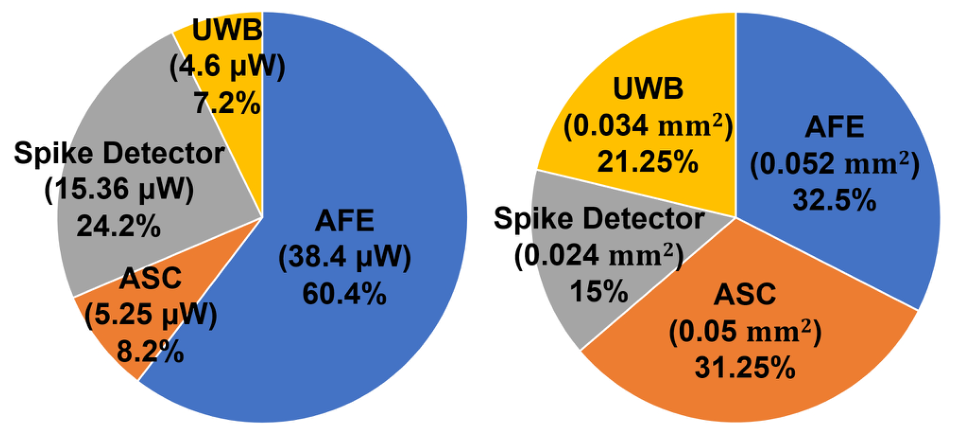
\includegraphics[width=\linewidth]{neuroseed_breakdown.png}
    \caption{Potenza (\SI{63{,}61}{\micro\watt}) e area attiva (\SI{0{,}16}{\milli\meter\squared}) in NeuroSEED~\cite{wu2026}.}
  \end{subfigure}
  \caption[Ripartizione di area e potenza: il peso dell'infrastruttura]{Evidenza quantitativa del peso dell'infrastruttura rispetto al core di calcolo: (a) distribuzione percentuale dell'area di silicio in ROLLS~\cite{qiao2015} (neuroni 0,47\% vs sinapsi 64,73\%, pad/altro $\sim 31\%$), DYNAPs~\cite{moradi2018} (core: memoria+PE/DEC 56,9\%, router 9,7\%, neuroni+sinapsi 22,8\%) e NeuroSEED~\cite{wu2026} (area attiva); (b) grafici a torta originali di potenza e area di NeuroSEED~\cite{wu2026}, in cui il front-end analogico AFE domina con il 60,4\% della potenza totale.}
  \label{fig:area_neuroseed}
\end{figure}

% --- FIGURA 4.3: Confronto logaritmico potenze di sistema ---
\begin{figure}[tb]
  \centering
  \resizebox{\textwidth}{!}{%
  \begin{tikzpicture}
    \begin{axis}[
      xbar,
      xmode=log,
      log origin=infty,
      bar width=11pt,
      width=12.4cm,
      height=5.9cm,
      xlabel={Potenza media di sistema in scala logaritmica (\si{\micro\watt})},
      ytick={1,2,3,4,5,6,7},
      yticklabels={
        {FPGA conv.\ (SVM/MLP)},
        {ROLLS (128k sin.\ plast.)},
        {Sharifshazileh (SNN+AFE)},
        {Xylo (SNN dig.\ + I/O)},
        {DYNAP-SE2 (iEEG 42--62ch)},
        {NeuroSEED (32ch AFE+TX)},
        {NET-TEN (solo core SNN)}
      },
      ymin=0.4, ymax=7.6,
      xmin=0.001, xmax=35000000,
      xmajorgrids=true,
      grid style={dashed, color=RuleGray},
      tick label style={font=\scriptsize},
      label style={font=\footnotesize},
      nodes near coords,
      point meta=explicit symbolic,
      every node near coord/.append style={font=\tiny\bfseries, anchor=west, xshift=3pt}
    ]
      \addplot[fill=black!55, draw=black] coordinates {
        (0.0035, 7) [\SI{3{,}50}{\nano\watt} (senza AFE/TX)]
        (63.61, 6) [\SI{63{,}61}{\micro\watt} (SoC completo)]
        (150, 5) [\SI{150}{\micro\watt} (\SI{2{,}8}{\micro\watt\per\ch})]
        (375.3, 4) [\SI{375{,}3}{\micro\watt} (senza AFE/ICA)]
        (555.6, 3) [\SI{555{,}6}{\micro\watt} (con AFE)]
        (4000, 2) [\SI{4}{\milli\watt} (apprend.\ on-line)]
        (220000, 1) [$160\text{--}\SI{284}{\milli\watt}$]
      };
    \end{axis}
  \end{tikzpicture}%
  }
  \caption[Confronto logaritmico delle potenze di sistema]{Confronto su scala logaritmica (nove ordini di grandezza) della potenza media dei sistemi analizzati: il passaggio dal solo nucleo SNN analogico (NET-TEN, \SI{3{,}5}{\nano\watt}) a un SoC impiantabile completo con acquisizione AFE e telemetria (NeuroSEED, \SI{63{,}6}{\micro\watt}) o a un processore SNN riconfigurabile (DYNAP-SE2, Xylo, ROLLS) ridimensiona drasticamente il guadagno del singolo neurone, pur conservando un margine decisivo ($10^2\text{--}10^3\times$) rispetto alle architetture digitali convenzionali su FPGA.}
  \label{fig:power_landscape}
\end{figure}

\FloatBarrier
\subsection{Sintesi dei colli di bottiglia e strategie di mitigazione}
\label{subsec:colli_bottiglia}

La Tabella~\ref{tab:colli_bottiglia} raccoglie in forma sintetica i quattro principali colli di bottiglia emersi dalla letteratura e le rispettive vie di soluzione architetturali e tecnologiche.

\begin{table}[htb]
  \centering
  \vspace{-4pt}
  \caption[Colli di bottiglia energetici e strategie di mitigazione]{Sintesi critica dei colli di bottiglia energetici e di area nei sistemi impiantabili basati su SNN e relative strategie di mitigazione emerse dalla bibliografia.}
  \label{tab:colli_bottiglia}
  \scriptsize
  \renewcommand{\arraystretch}{0.98}
  \setlength{\tabcolsep}{4pt}
  \begin{tabularx}{\textwidth}{@{}L{2.3cm} L{3.25cm} Y Y@{}}
    \toprule
    \textbf{Blocco critico} & \textbf{Evidenza quantitativa} & \textbf{Origine fisica / architetturale} & \textbf{Strategie di mitigazione} \\
    \midrule
    \textbf{Front-end di acquisizione (AFE)} & NeuroSEED: \SI{38{,}4}{\micro\watt} (\textbf{60,4\%} della potenza del SoC; 32,5\% area)~\cite{wu2026}. & Limite del rumore termico in banda (compromesso $g_m/I_D$ e NEF) e cancellazione offset DC elettrodico ($\pm\SI{50}{\milli\volt}$). & Multiplexing diretto TDM + LNA \emph{current-reuse} in sottosoglia (NEF 2,1) + servo-loop digitale EDO + codifica ADM/ASC integrata~\cite{wu2026, bartels2025}. \\
    \textbf{Sinapsi e memoria pesi} & ROLLS: \textbf{64,73\%} area per sinapsi vs 0,47\% neuroni~\cite{qiao2015}; NET-TEN: ritenzione $C_w$ solo decine di ms~\cite{ronchini2023}. & Fan-in/fan-out elevato; perdita di carica sui condensatori analogici; costo delle celle SRAM/bistabili. & Condivisione DPI per riga~\cite{qiao2015}; topologie sparse e pesi quantizzati/costanti~\cite{ronchini2023, bartels2025}; memorie non volatili emergenti (ReRAM / memristori)~\cite{moradi2018, indiveri2011}. \\
    \textbf{Interconnessioni e routing (CAM/AER)} & DYNAPs: broadcast CAM \textbf{\SI{6{,}84}{\nano\joule}} (\SI{1{,}8}{\volt}) / \textbf{\SI{2{,}2}{\nano\joule}} (\SI{1{,}3}{\volt}), ovvero $7{,}7\text{--}8{,}5\times$ la gen.\ dello spike~\cite{moradi2018}. & Carica/scarica delle linee di ricerca e \emph{match-line} su grandi array di CAM e bus digitali. & Routing gerarchico a due stadi basato su tag (Eq.~\ref{eq:dynaps_mem}); scalatura a nodi avanzati (\SI{28}{\nano\meter} FDSOI)~\cite{moradi2018}; reti dedicate senza bus AER dove non serve riconfigurabilità~\cite{ronchini2023}. \\
    \textbf{Variabilità (\emph{mismatch}) e post-processing} & DYNAP-SE2: CV bias 20--30\%~\cite{bartels2025}; NET-TEN: 4/10 canali utili; Xylo: $-3{,}5\text{--}4{,}3\%$ acc.\ da quant.\ 8 bit~\cite{li2024}. & Dispersione esponenziale di $I_D$ in sottosoglia ($\Delta V_{\mathrm{th}}$) e sensibilità alla densità di codifica. & Sovradimensionamento mirato (ROLLS: 9,4\%~\cite{qiao2015}); reti a popolazione/topologia robusta (NLNG~\cite{bartels2025}); apprendimento omeostatico on-chip; contatori ultra-low-power on-chip~\cite{ronchini2023}. \\
    \bottomrule
  \end{tabularx}
  \vspace{-6pt}
\end{table}

\FloatBarrier
\vspace{-4pt}
\subsection{Verdetto conclusivo}
\label{subsec:verdetto}

\begin{criticaBox}[top=5pt, bottom=5pt, before skip=2pt, after skip=2pt]{Conclusione critica: le SNN offrono davvero un vantaggio energetico concreto negli impianti biomedicali?}
{\footnotesize\setlength{\baselineskip}{10.5pt}
L'analisi comparativa integrata conduce a una risposta netta e articolata in due parti complementari:
\begin{enumerate}[topsep=2pt, itemsep=1.5pt]
  \item \textbf{Sì, il consumo dell'infrastruttura ridimensiona drasticamente il beneficio isolato del singolo neurone ultra-low-power.} Parlare di ``processori da pochi nanowatt'' guardando solo il core analogico (come i \SI{3{,}50}{\nano\watt} di NET-TEN) è fuorviante se non si include il costo del resto della catena: in un dispositivo impiantabile reale, il front-end analogico di acquisizione (60,4\% della potenza in NeuroSEED), le sinapsi (64,7\% dell'area in ROLLS) e soprattutto la memoria associativa e le interconnessioni di routing (fino all'87--90\% dell'energia per evento in DYNAPs) dominano di \textbf{uno fino a quattro ordini di grandezza} rispetto al consumo intrinseco del soma neuronale (Figura~\ref{fig:power_landscape}).
  \item \textbf{Ciononostante, il paradigma SNN/\emph{event-driven} offre un vantaggio energetico e sistemistico concreto e decisivo, a patto che sia co-progettato a livello di intero sistema.} Il vero guadagno delle SNN impiantabili non deriva tanto dal risparmiare qualche picojoule nel singolo neurone, bensì dal loro impatto a cascata sull'intera architettura del dispositivo:
  \begin{itemize}[topsep=1.5pt, itemsep=1pt]
    \item \textbf{Abbattimento della telemetria wireless:} elaborare ed estrarre eventi localmente comprime il flusso dati di oltre $500\times$ (NeuroSEED riduce il trasmettitore IR-UWB a soli \SI{4{,}6}{\micro\watt}, appena il 7,2\% del chip), risolvendo il collo di bottiglia energetico più critico delle interfacce multicanale ad alta densità.
    \item \textbf{Eliminazione di buffer, ADC Nyquist continui e clock globali:} l'elaborazione asincrona in \emph{streaming} consente latenze di decine di millisecondi (essenziali per la neuromodulazione \emph{closed-loop} dell'epilessia) e un consumo strettamente modulato dall'occorrenza di eventi patologici, con un guadagno di $10^2\text{--}10^3\times$ rispetto a implementazioni convenzionali su FPGA o microprocessori general-purpose.
  \end{itemize}
\end{enumerate}
In prospettiva, la maturità clinica dei sistemi biomedicali impiantabili neuromorfici non dipenderà quindi dall'ulteriore miniaturizzazione isolata del neurone LIF/AdEx, bensì dalla \textbf{co-progettazione olistica \emph{end-to-end}} di front-end compatti a basso rumore (TDM/ADM/ASC), topologie SNN sparse intrinsecamente robuste al \emph{mismatch} (o capaci di adattamento omeostatico locale), stadi di decisione/classificazione interamente on-chip e tecnologie di memoria non volatile integrata (come ReRAM) capaci di abbattere il costo energetico di sinapsi e routing.
}
\end{criticaBox}

\clearpage

% ==============================================================================
% BIBLIOGRAFIA
% ==============================================================================
\addcontentsline{toc}{section}{Bibliografia}
\printbibliography[title={Bibliografia}]

\end{document}
